\documentclass[a4paper]{report}

\usepackage[utf8]{inputenc}
\usepackage{graphicx}
\usepackage{url}
\usepackage{import}
\usepackage{titlesec}
\usepackage{pgfgantt}
\usepackage{geometry}
\usepackage{changepage}
\usepackage{tocbibind} % adds bibliography to table of contents
\usepackage[most]{tcolorbox}
\usepackage{lmodern}
\usepackage{lipsum}
\usepackage{tikz-qtree}
\usepackage{tikz}
\usepackage{algorithm2e}
\usepackage{listings}
\usepackage{booktabs}
%\usepackage{parskip}


\SetKw{Continue}{continue}
\SetKw{Break}{break}

\titleformat{\chapter}{\normalfont\huge\bfseries}{\thechapter}{1em}{}


\title{Butter - a decentralised application framework}
\date{\today}

\begin{document}
    \maketitle

    \begin{abstract}
        Peer-to-peer (p2p) systems have some interesting properties in regard to scalability and dependability, due to
        their decentralised nature. They address many of the pitfalls of centralised architectures such as cost of
        infrastructure and single points of failure, resulting in fault-tolerant networks that can behave autonomously.
        Many of the current efforts to design peer-to-peer systems use structured elements which improve the performance
        but re-introduce some of the precariousness present in centralised systems. Butter is a peer-to-peer framework
        loosely inspired by other project such as Gnutella, JXTA and libp2p, its goal is to explore what is achievable
        in unstructured p2p networks. Each of the problems in building a p2p middleware corresponds to a module of the
        framework. Peer discovery is handled using a multicast protocol, we introduce a unique approach to known host
        management optimising for diversity and describe the design of the Network Address Translation (NAT) traversal
        and internet discovery module. Finally, we present the overlay design that enables persistent information and
        information retrieval by introducing Peer Content Groups (PCG) and Random Breadth-first search mechanisms
        respectively. An analysis of different decentralised application services is provided arguing the benefits and
        shortfalls of decentralised architectures. The work provides a complete overview of the project, covering all
        aspects including background information, related projects, management challenges, design, testing and
        evaluation of Butter. We describe the technical achievements, give direction as to the next stage of the
        development and conclude that peer-to-peer architectures are particularly well suited for public information
        and communication services but designing these systems can be more complex than their centralised counterparts.\\

        \noindent\textbf{Keywords:} Networks, Distributed systems, Decentralisation, Peer-to-peer (p2p), Dependability, Availability, Middleware, Framework
    \end{abstract}

    \tableofcontents

    \chapter{Introduction}
\label{ch:introduction}

% The introduction needs to:
% - Provide a broad background or context to the field or discipline and topic, to orient the reader so that they understand what follows
% - Setup the issue – What’s the problem? What is the scope and limitation existing solutions?
% - State your contributions or argument - What are you bringing that’s new?
% - Signpost and outline the structure of your work

% --- Orienting the reader from the top-down - distributed systems ---
In his book \textit{Distributed Systems: Principles and Paradigms}, Tanenbaum discusses the difficultly in accurately characterising distributed systems and makes allusions to the generally poor definitions often given in the literature, stating that ``none of them [are] satisfactory, and none of them [are] in agreement with any of the others". Distributed systems are so prevalent, it can be difficult to come up with a definition that captures them all. Tanembaum, hence, provides a loose characterisation of a distributed system as a ``collection of independent computers that appears to its users as a single coherent system". This characterisation is sufficient within the context of this work. In this report, we will be focused on exploring decentralised systems, specifically with a peer-to-peer (p2p) architecture and introduce the main output of this project: Butter.\cite{tanenbaum2007distributed}


\section{Background}
\label{sec:background}

In this section we shall be providing some background on distributed systems, distributed architectures and how they can give rise to centralised and decentralised properties, overlay and peer-to-peer networks.

\subsection{Distributed systems \& architectures}
\label{subsec:distributedSystemsArchitectures}

Distributed systems have a few notable characteristics. Firstly, the ``differences between the various computers [constituting the system] and the way in which they communicate are mostly hidden from the user" meaning that the underlying organisation of the system is abstracted away from the user. Secondly, the ``users and applications can interact with a distributed system in a continuous and uniform way, regardless of when and where the interactions take place", which makes them well suited to deliver application services over the internet. Finally, distributed behaviour often lies in-between logical application layers of the system hence it is often referred to as the distributed behaviour middleware.\cite{tanenbaum2007distributed}

\begin{figure}[ht]
    \centering
    \documentclass[main.tex]{subfiles}

\pagestyle{empty}
\begin{document}

    \tikzset{edge from parent/.style=
            {draw, edge from parent path={(\tikzparentnode.south)
        -- +(0,-8pt)
        -| (\tikzchildnode)}},
        blank/.style={draw=none}}
    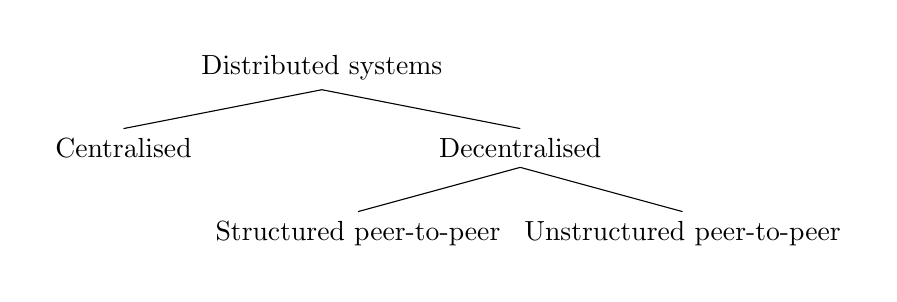
\begin{tikzpicture}
        \matrix
        {
            \node{\Tree
                [.{Distributed systems}
                    [.Centralised ]
                    [.Decentralised
                        [.{Structured peer-to-peer} ]
                        [.{Unstructured peer-to-peer} ]
                    ]
                ]
            };\\
        };
    \end{tikzpicture}

\end{document}

    \caption{Distributed systems taxonomy}
    \label{fig:distributed_taxonomy}
\end{figure}

% --- Taxonomy of distributed systems architecture ---
Distributes systems can be organised in several ways depending on how the software components are placed and interact, this leads to an instance of a system architecture\cite{bass2003architecture}. Figure~\ref{fig:distributed_taxonomy} illustrates the taxonomy of distributed systems in terms of the different possible architectures.

% --- Introducing the paradigm of clients and servers ---
In this report, like many other works of distributed systems, we will be thinking in the terms of \textit{clients} initiating connections to fulfil requests from \textit{servers}. A server is a ``process implementing a specific service" such as a database while a ``client is a process that requests a service from a server by sending it a request and subsequently waiting for the server’s reply". Thinking in these terms will help us reason and manage the complexity while discussing the system.\cite{tanenbaum2007distributed}

% --- Introducing centralised vs. decentralised architecture ---
% Vertically distributed architecture
When a system is distributed into logical layers, such as a database, processing components and user-interface, the distribution is vertical as the data flows from one layer to the next\cite{tanenbaum2007distributed}. In this architectural style, the users interface with the service through an endpoint, the top layer of the vertical stack. The user-level clients are distinct, unique and mutually exclusive from the service providing nodes.

% Horizontally distributed architecture
While having a vertical distribution, from a systems' management perspective, can help to logically and physically split system components across machines to provide a service, it is not the only way of organising a distributed system. For instance, distributing clients and servers in such a way that they operate based on their own data set (i.e., their view of the system), thus balancing load, is referred to as horizontal distribution. This distribution style is what gives rise to decentralised systems.\cite{tanenbaum2007distributed}

\subsection{Centralisation \& decentralisation}
\label{subsec:centralisationVsDecentralisation}

% Centralisation
One of the pitfalls of non-distributed systems (i.e. just a single process) or a system with at least one vertical step in its distribution is that they introduce centralisation. Centralisation is when there are unique central processes that others depend on to fulfil a service\cite{raval2016decentralised}. If a serving component of the system fails, clients become unable to access information and interact with the service. This precariousness comes about due to the inherent inter-dependability of the system subcomponents. For example, a typical architecture for a web application includes a vertically distributed database, data processing server and user-interface. The resulting system is distributed yet centralised, as if any one of the subcomponents should fail, e.g. the database, users would be unable to interact with the service. Large, heavily centralised systems consist of few servers relative to the number of clients, hence if a server becomes unavailable, a large number of clients may be unable to function. In some critical systems, where information availability is of paramount importance, a centralised system is at a higher risk of failure making the system less dependable.

\begin{figure}[ht]
    \centering
    \resizebox{\textwidth}{!}{
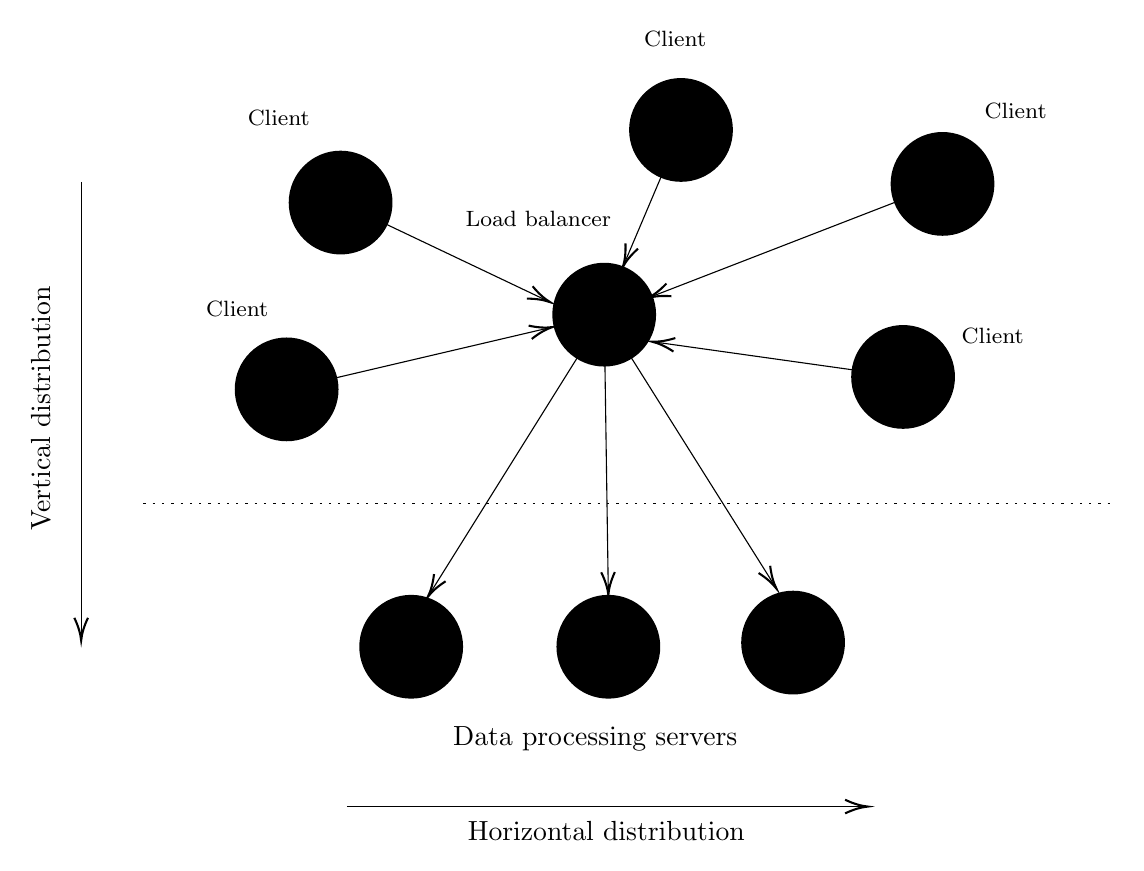
\begin{tikzpicture}[x=0.75pt,y=0.75pt,yscale=-1,xscale=1]
%uncomment if require: \path (0,451); %set diagram left start at 0, and has height of 451

%Shape: Circle [id:dp21625012916250363] 
\draw  [draw opacity=0][fill={rgb, 255:red, 0; green, 0; blue, 0 }  ,fill opacity=1 ] (307,172) .. controls (307,158.19) and (318.19,147) .. (332,147) .. controls (345.81,147) and (357,158.19) .. (357,172) .. controls (357,185.81) and (345.81,197) .. (332,197) .. controls (318.19,197) and (307,185.81) .. (307,172) -- cycle ;
%Shape: Circle [id:dp4205702906990445] 
\draw  [draw opacity=0][fill={rgb, 255:red, 0; green, 0; blue, 0 }  ,fill opacity=1 ] (451,202) .. controls (451,188.19) and (462.19,177) .. (476,177) .. controls (489.81,177) and (501,188.19) .. (501,202) .. controls (501,215.81) and (489.81,227) .. (476,227) .. controls (462.19,227) and (451,215.81) .. (451,202) -- cycle ;
%Shape: Circle [id:dp1834367315754477] 
\draw  [draw opacity=0][fill={rgb, 255:red, 0; green, 0; blue, 0 }  ,fill opacity=1 ] (470,109) .. controls (470,95.19) and (481.19,84) .. (495,84) .. controls (508.81,84) and (520,95.19) .. (520,109) .. controls (520,122.81) and (508.81,134) .. (495,134) .. controls (481.19,134) and (470,122.81) .. (470,109) -- cycle ;
%Shape: Circle [id:dp8062304220658076] 
\draw  [draw opacity=0][fill={rgb, 255:red, 0; green, 0; blue, 0 }  ,fill opacity=1 ] (344,83) .. controls (344,69.19) and (355.19,58) .. (369,58) .. controls (382.81,58) and (394,69.19) .. (394,83) .. controls (394,96.81) and (382.81,108) .. (369,108) .. controls (355.19,108) and (344,96.81) .. (344,83) -- cycle ;
%Shape: Circle [id:dp3524619405588886] 
\draw  [draw opacity=0][fill={rgb, 255:red, 0; green, 0; blue, 0 }  ,fill opacity=1 ] (214,332) .. controls (214,318.19) and (225.19,307) .. (239,307) .. controls (252.81,307) and (264,318.19) .. (264,332) .. controls (264,345.81) and (252.81,357) .. (239,357) .. controls (225.19,357) and (214,345.81) .. (214,332) -- cycle ;
%Shape: Circle [id:dp2671841919001372] 
\draw  [draw opacity=0][fill={rgb, 255:red, 0; green, 0; blue, 0 }  ,fill opacity=1 ] (309,332) .. controls (309,318.19) and (320.19,307) .. (334,307) .. controls (347.81,307) and (359,318.19) .. (359,332) .. controls (359,345.81) and (347.81,357) .. (334,357) .. controls (320.19,357) and (309,345.81) .. (309,332) -- cycle ;
%Shape: Circle [id:dp3753155355544049] 
\draw  [draw opacity=0][fill={rgb, 255:red, 0; green, 0; blue, 0 }  ,fill opacity=1 ] (398,330) .. controls (398,316.19) and (409.19,305) .. (423,305) .. controls (436.81,305) and (448,316.19) .. (448,330) .. controls (448,343.81) and (436.81,355) .. (423,355) .. controls (409.19,355) and (398,343.81) .. (398,330) -- cycle ;
%Shape: Circle [id:dp9331094894799612] 
\draw  [draw opacity=0][fill={rgb, 255:red, 0; green, 0; blue, 0 }  ,fill opacity=1 ] (180,118) .. controls (180,104.19) and (191.19,93) .. (205,93) .. controls (218.81,93) and (230,104.19) .. (230,118) .. controls (230,131.81) and (218.81,143) .. (205,143) .. controls (191.19,143) and (180,131.81) .. (180,118) -- cycle ;
%Shape: Circle [id:dp15130202099269585] 
\draw  [draw opacity=0][fill={rgb, 255:red, 0; green, 0; blue, 0 }  ,fill opacity=1 ] (154,208) .. controls (154,194.19) and (165.19,183) .. (179,183) .. controls (192.81,183) and (204,194.19) .. (204,208) .. controls (204,221.81) and (192.81,233) .. (179,233) .. controls (165.19,233) and (154,221.81) .. (154,208) -- cycle ;
%Straight Lines [id:da6549389594791377] 
\draw    (205,118) -- (304.19,165.14) ;
\draw [shift={(306,166)}, rotate = 205.42] [color={rgb, 255:red, 0; green, 0; blue, 0 }  ][line width=0.75]    (10.93,-3.29) .. controls (6.95,-1.4) and (3.31,-0.3) .. (0,0) .. controls (3.31,0.3) and (6.95,1.4) .. (10.93,3.29)   ;
%Straight Lines [id:da41842174722404835] 
\draw    (179,208) -- (305.05,178.46) ;
\draw [shift={(307,178)}, rotate = 166.81] [color={rgb, 255:red, 0; green, 0; blue, 0 }  ][line width=0.75]    (10.93,-3.29) .. controls (6.95,-1.4) and (3.31,-0.3) .. (0,0) .. controls (3.31,0.3) and (6.95,1.4) .. (10.93,3.29)   ;
%Straight Lines [id:da5248390031839211] 
\draw    (369,83) -- (341.78,147.16) ;
\draw [shift={(341,149)}, rotate = 292.99] [color={rgb, 255:red, 0; green, 0; blue, 0 }  ][line width=0.75]    (10.93,-3.29) .. controls (6.95,-1.4) and (3.31,-0.3) .. (0,0) .. controls (3.31,0.3) and (6.95,1.4) .. (10.93,3.29)   ;
%Straight Lines [id:da3704088342799581] 
\draw    (495,109) -- (354.86,163.28) ;
\draw [shift={(353,164)}, rotate = 338.83] [color={rgb, 255:red, 0; green, 0; blue, 0 }  ][line width=0.75]    (10.93,-3.29) .. controls (6.95,-1.4) and (3.31,-0.3) .. (0,0) .. controls (3.31,0.3) and (6.95,1.4) .. (10.93,3.29)   ;
%Straight Lines [id:da45067791114233546] 
\draw    (476,202) -- (356.98,185.28) ;
\draw [shift={(355,185)}, rotate = 8] [color={rgb, 255:red, 0; green, 0; blue, 0 }  ][line width=0.75]    (10.93,-3.29) .. controls (6.95,-1.4) and (3.31,-0.3) .. (0,0) .. controls (3.31,0.3) and (6.95,1.4) .. (10.93,3.29)   ;
%Straight Lines [id:da675702571699395] 
\draw    (332,172) -- (248.06,306.3) ;
\draw [shift={(247,308)}, rotate = 302.01] [color={rgb, 255:red, 0; green, 0; blue, 0 }  ][line width=0.75]    (10.93,-3.29) .. controls (6.95,-1.4) and (3.31,-0.3) .. (0,0) .. controls (3.31,0.3) and (6.95,1.4) .. (10.93,3.29)   ;
%Straight Lines [id:da19941562676333713] 
\draw    (332,172) -- (333.97,305) ;
\draw [shift={(334,307)}, rotate = 269.15] [color={rgb, 255:red, 0; green, 0; blue, 0 }  ][line width=0.75]    (10.93,-3.29) .. controls (6.95,-1.4) and (3.31,-0.3) .. (0,0) .. controls (3.31,0.3) and (6.95,1.4) .. (10.93,3.29)   ;
%Straight Lines [id:da44186877727070717] 
\draw    (332,172) -- (413.94,302.31) ;
\draw [shift={(415,304)}, rotate = 237.84] [color={rgb, 255:red, 0; green, 0; blue, 0 }  ][line width=0.75]    (10.93,-3.29) .. controls (6.95,-1.4) and (3.31,-0.3) .. (0,0) .. controls (3.31,0.3) and (6.95,1.4) .. (10.93,3.29)   ;
%Straight Lines [id:da00352783652063271] 
\draw  [dash pattern={on 0.84pt off 2.51pt}]  (110,263) -- (578,263) ;
%Straight Lines [id:da8513516782413686] 
\draw    (80,108) -- (80,327) ;
\draw [shift={(80,329)}, rotate = 270] [color={rgb, 255:red, 0; green, 0; blue, 0 }  ][line width=0.75]    (10.93,-3.29) .. controls (6.95,-1.4) and (3.31,-0.3) .. (0,0) .. controls (3.31,0.3) and (6.95,1.4) .. (10.93,3.29)   ;
%Straight Lines [id:da5994970572513846] 
\draw    (208,409) -- (457,409) ;
\draw [shift={(459,409)}, rotate = 180] [color={rgb, 255:red, 0; green, 0; blue, 0 }  ][line width=0.75]    (10.93,-3.29) .. controls (6.95,-1.4) and (3.31,-0.3) .. (0,0) .. controls (3.31,0.3) and (6.95,1.4) .. (10.93,3.29)   ;

% Text Node
\draw (264,121) node [anchor=north west][inner sep=0.75pt]   [align=left] {{\footnotesize Load balancer}};
% Text Node
\draw (159,72) node [anchor=north west][inner sep=0.75pt]   [align=left] {{\footnotesize Client}};
% Text Node
\draw (350,34) node [anchor=north west][inner sep=0.75pt]   [align=left] {{\footnotesize Client}};
% Text Node
\draw (514,69) node [anchor=north west][inner sep=0.75pt]   [align=left] {{\footnotesize Client}};
% Text Node
\draw (503,177) node [anchor=north west][inner sep=0.75pt]   [align=left] {{\footnotesize Client}};
% Text Node
\draw (139,164) node [anchor=north west][inner sep=0.75pt]   [align=left] {{\footnotesize Client}};
% Text Node
\draw (258,369) node [anchor=north west][inner sep=0.75pt]   [align=left] {Data processing servers};
% Text Node
\draw (54.5,277.5) node [anchor=north west][inner sep=0.75pt]  [rotate=-270] [align=left] {Vertical distribution};
% Text Node
\draw (265,415) node [anchor=north west][inner sep=0.75pt]   [align=left] {Horizontal distribution};


\end{tikzpicture}
}

    \caption{Example of a both vertical and horizontally distributed architecture}
    \label{fig:vertHorArch}
\end{figure}

A subtle design to note, is that a system may still be centralised if the underlying server infrastructure is itself horizontally distributed. For example, many cloud services lie behind load balancing servers. The load balancing server does not itself provide the core service but provide a supporting role in balancing server load\cite{rajagopalan2020load}. While the underlying system running the service is horizontally distributed, there is still only a single endpoint with which the client interacts, that of the load balancing server. This is illustrated in Figure~\ref{fig:vertHorArch}, where there is a single publicly available load balancing server which acts an as endpoint for the overall service.

A good example of the risks caused by a centralised service is the `2021 Facebook outage' which made Facebook, WhatsApp and Instagram unavailable for over six hours on October 4th 2021\cite{heath2021facebook}. An engineer made a configuration error while updating a router protocol resulting in the Border Gateway Protocol (BGP)\cite{feamster2005detecting} ``disconnecting Facebook data centres globally"\cite{janardhan2021meta}. This, in turn, prevented Facebook's main DNS server from connecting to other nodes. Facebook has a globally distributed architecture, with backup databases and data processing servers, but users still interact with the services through their domain. If users are unable to resolve the \verb+facebook.com+ domain, they cannot access the underlying service regardless of whether their internal architecture is highly horizontally distributed. This was further worsened by engineers being unable to access the buildings to fix the configuration error as the card authentication system also relied on Facebook's own DNS servers\cite{heath2021facebook}. This case study shows that high levels of centralisation and dependency can be risk-prone and suggests that relying on large centralised cloud services to provide communication services may be unwise.

Decentralisation, which occurs from horizontally distributed architectures, can offer some distinct advantages over a centralised design for delivering certain services. Given that decentralised systems are devoid of hierarchical organisation or centralised control\cite{lua2005survey}, there is no single-point of failure\cite{raval2016decentralised}, however, this comes at a significant cost of performance relative to the centralised equivalent providing the same service. Notably, maintaining information across several nodes comes at the cost of time complexity (as several nodes must process the information), space complexity (as some form of redundancy is often introduced) and most significantly message complexity (as nodes need to communicate with each other to determine their partial views of the system). Designing efficient decentralised protocols is of paramount importance for a decentralised system to effectively deliver its service.

\subsection{Overlay networks}
\label{subsec:overlayNetworks}

\begin{figure}[ht]
    \centering
    % \tikzset{every picture/.style={line width=0.75pt}} %set default line width to 0.75pt        

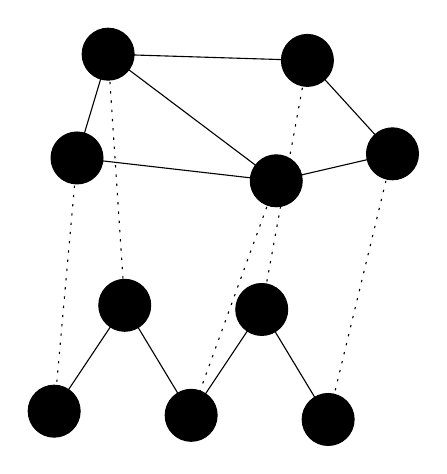
\begin{tikzpicture}[x=0.75pt,y=0.75pt,yscale=-1,xscale=1]
%uncomment if require: \path (0,300); %set diagram left start at 0, and has height of 300

%Shape: Circle [id:dp6061502443078786] 
\draw  [fill={rgb, 255:red, 0; green, 0; blue, 0 }  ,fill opacity=1 ] (125,118.5) .. controls (125,111.6) and (130.6,106) .. (137.5,106) .. controls (144.4,106) and (150,111.6) .. (150,118.5) .. controls (150,125.4) and (144.4,131) .. (137.5,131) .. controls (130.6,131) and (125,125.4) .. (125,118.5) -- cycle ;
%Shape: Circle [id:dp36264343921365794] 
\draw  [fill={rgb, 255:red, 0; green, 0; blue, 0 }  ,fill opacity=1 ] (140,68.5) .. controls (140,61.6) and (145.6,56) .. (152.5,56) .. controls (159.4,56) and (165,61.6) .. (165,68.5) .. controls (165,75.4) and (159.4,81) .. (152.5,81) .. controls (145.6,81) and (140,75.4) .. (140,68.5) -- cycle ;
%Shape: Circle [id:dp9971317502608965] 
\draw  [fill={rgb, 255:red, 0; green, 0; blue, 0 }  ,fill opacity=1 ] (236,71.5) .. controls (236,64.6) and (241.6,59) .. (248.5,59) .. controls (255.4,59) and (261,64.6) .. (261,71.5) .. controls (261,78.4) and (255.4,84) .. (248.5,84) .. controls (241.6,84) and (236,78.4) .. (236,71.5) -- cycle ;
%Shape: Circle [id:dp9106166132377405] 
\draw  [fill={rgb, 255:red, 0; green, 0; blue, 0 }  ,fill opacity=1 ] (277,116.5) .. controls (277,109.6) and (282.6,104) .. (289.5,104) .. controls (296.4,104) and (302,109.6) .. (302,116.5) .. controls (302,123.4) and (296.4,129) .. (289.5,129) .. controls (282.6,129) and (277,123.4) .. (277,116.5) -- cycle ;
%Shape: Circle [id:dp5541002056383258] 
\draw  [fill={rgb, 255:red, 0; green, 0; blue, 0 }  ,fill opacity=1 ] (221,129.5) .. controls (221,122.6) and (226.6,117) .. (233.5,117) .. controls (240.4,117) and (246,122.6) .. (246,129.5) .. controls (246,136.4) and (240.4,142) .. (233.5,142) .. controls (226.6,142) and (221,136.4) .. (221,129.5) -- cycle ;
%Straight Lines [id:da3029168780037723] 
\draw    (152.5,68.5) -- (248.5,71.5) ;
%Straight Lines [id:da46957863774592223] 
\draw    (233.5,129.5) -- (152.5,68.5) ;
%Straight Lines [id:da9097415304582196] 
\draw    (248.5,71.5) -- (289.5,116.5) ;
%Straight Lines [id:da2061802483174313] 
\draw    (137.5,118.5) -- (233.5,129.5) ;
%Straight Lines [id:da9316247214989568] 
\draw    (233.5,129.5) -- (289.5,116.5) ;
%Straight Lines [id:da31757544534246873] 
\draw    (152.5,68.5) -- (137.5,118.5) ;
%Shape: Circle [id:dp39230600009532957] 
\draw  [fill={rgb, 255:red, 0; green, 0; blue, 0 }  ,fill opacity=1 ] (114,240.5) .. controls (114,233.6) and (119.6,228) .. (126.5,228) .. controls (133.4,228) and (139,233.6) .. (139,240.5) .. controls (139,247.4) and (133.4,253) .. (126.5,253) .. controls (119.6,253) and (114,247.4) .. (114,240.5) -- cycle ;
%Shape: Circle [id:dp6725211407093591] 
\draw  [fill={rgb, 255:red, 0; green, 0; blue, 0 }  ,fill opacity=1 ] (148,189.5) .. controls (148,182.6) and (153.6,177) .. (160.5,177) .. controls (167.4,177) and (173,182.6) .. (173,189.5) .. controls (173,196.4) and (167.4,202) .. (160.5,202) .. controls (153.6,202) and (148,196.4) .. (148,189.5) -- cycle ;
%Shape: Circle [id:dp534352110903068] 
\draw  [fill={rgb, 255:red, 0; green, 0; blue, 0 }  ,fill opacity=1 ] (214,191.5) .. controls (214,184.6) and (219.6,179) .. (226.5,179) .. controls (233.4,179) and (239,184.6) .. (239,191.5) .. controls (239,198.4) and (233.4,204) .. (226.5,204) .. controls (219.6,204) and (214,198.4) .. (214,191.5) -- cycle ;
%Shape: Circle [id:dp5705459677432333] 
\draw  [fill={rgb, 255:red, 0; green, 0; blue, 0 }  ,fill opacity=1 ] (246,244.5) .. controls (246,237.6) and (251.6,232) .. (258.5,232) .. controls (265.4,232) and (271,237.6) .. (271,244.5) .. controls (271,251.4) and (265.4,257) .. (258.5,257) .. controls (251.6,257) and (246,251.4) .. (246,244.5) -- cycle ;
%Shape: Circle [id:dp4884732451202879] 
\draw  [fill={rgb, 255:red, 0; green, 0; blue, 0 }  ,fill opacity=1 ] (180,242.5) .. controls (180,235.6) and (185.6,230) .. (192.5,230) .. controls (199.4,230) and (205,235.6) .. (205,242.5) .. controls (205,249.4) and (199.4,255) .. (192.5,255) .. controls (185.6,255) and (180,249.4) .. (180,242.5) -- cycle ;
%Straight Lines [id:da5435068621925384] 
\draw    (160.5,189.5) -- (126.5,240.5) ;
%Straight Lines [id:da40058310101255523] 
\draw    (160.5,189.5) -- (192.5,242.5) ;
%Straight Lines [id:da745960373491508] 
\draw    (226.5,191.5) -- (192.5,242.5) ;
%Straight Lines [id:da9636103089067328] 
\draw    (226.5,191.5) -- (258.5,244.5) ;
%Straight Lines [id:da026025176740933853] 
\draw  [dash pattern={on 0.84pt off 2.51pt}]  (137.5,118.5) -- (126.5,240.5) ;
%Straight Lines [id:da8574677477453254] 
\draw  [dash pattern={on 0.84pt off 2.51pt}]  (152.5,68.5) -- (160.5,189.5) ;
%Straight Lines [id:da45830762125909896] 
\draw  [dash pattern={on 0.84pt off 2.51pt}]  (248.5,71.5) -- (226.5,191.5) ;
%Straight Lines [id:da692101028265002] 
\draw  [dash pattern={on 0.84pt off 2.51pt}]  (233.5,129.5) -- (192.5,242.5) ;
%Straight Lines [id:da20439957038676881] 
\draw  [dash pattern={on 0.84pt off 2.51pt}]  (289.5,116.5) -- (258.5,244.5) ;




\end{tikzpicture}
    \caption{Overlay network of five nodes on top of another network}
    \label{fig:overlay_network}
\end{figure}

% --- What is overlay network ---
An overlay is a logical network that is implemented on top of some underlying network (see Figure~\ref{fig:overlay_network}). There is a one-to-one mapping between the nodes in each layer, i.e., each node in the overlay is associated with a node in the underlying network. The overlay nodes process and forward packets in an application-specific way. There can exist several overlay networks on top of the same underlying network each implementing its own application-specific behaviour and overlays can also be nested, one on top of another.\cite{peterson2012networks}

\subsection{Peer-to-peer systems}
\label{subsec:p2pSystems}

% --- What is peer-to-peer? ---
In this work we will focus on a horizontally distributed system architecture known as peer-to-peer. Peers are ``distributed computational entities each of which are considered equally important in terms of initiating an interaction and each of which provides its own resources"\cite{bass2003architecture}. The peers cooperate and collaborate to provide a service; often to a distributed community of users. In a peer-to-peer system, nodes behaves both as clients and servers. This symmetry supports community resource sharing, however for effective service delivery a fault-tolerant design is required\cite{lua2005survey}.

Peer-to-peer systems are both a ``social and technical phenomenon"\cite{ripeanu2001peer}. They allow for community resource aggregation to share storage space (e.g. Gnutella, Napster, BitTorrent), CPU cycles (e.g. \verb+SETI@Home+), or support collaborative environments (e.g. Groove) hence p2p networks are often used to support community projects that may otherwise be unachievable. There are several factors that have fostered the growth of such systems: first, the low cost and high availability of large numbers of computing and storage resources, second, increased network connectivity\cite{ripeanu2001peer} as well as a desire become less dependent on cloud services\cite{raval2016decentralised}.

Peers form self-organising networks that are `overlayed' on underlying network infrastructure. By their nature, they have the advantage of providing services with ``massive scalability, and fault-tolerance"\cite{lua2005survey}. However, because peer-to-peer systems are decentralised (i.e., fully horizontally distributed) managing data consistency as well as data and service availability is more complex. In many cases it is ``difficult to provide guarantees with peer-to-peer systems because the peers come and go"\cite{bass2003architecture} we refer to this process as `churn'\cite{baldoni2005churn}.

% A peer-to-peer architecture can help address some of the pitfalls of the traditional centralised client-server model such as reducing cost barrier to entry for server infrastructure while being highly scalable, removing single-points of failure and hence targets for malicious attacks and censorship\cite{raval_2016}.

% Include this stuff from the jxta paper as its good!

% There is substance to peer-to-peer technologies as they have the ability to ``greatly increase the utilisation of three valuable and fundamental Internet assets: information, bandwidth, and computing resources All of these are vastly underutilised at this time, partly due to the traditional client-server computing model"\cite{jxta}. 

% They argues it was important to develop p2p systems as ``miles of new fiber have been installed, the new bandwidth gets little use if everyone goes to Yahoo for content and to eBay for auctions. Instead, hot spots just get hotter while cold pipes remain cold"\cite{jxta} and ``new processors and storage devices continue to break records in speed and capacity, supporting more powerful personal devices throughout the network. However, computation continues to accumulate around data centres, which have to increase their workloads at a crippling pace, thus putting immense pressure on space and power consumption"

% ``p2p technologies can adopt a network-based computing style that neither excludes nor inherently depends on centralised control points. This style can enhance the overall reliability and fault tolerance of computing systems"

% Unlike traditional distributed systems, p2p networks aim to aggregate large numbers of computers that join and leave the network frequently and that might not have permanent network (IP) addresses. In pure p2p systems, individual computers communicate directly with each other and share information and resources without using dedicated servers. A common characteristic of this new breed of systems is that they build, at the application level, a virtual network with its own routing mechanisms. The topology of the virtual network and the routing mechanisms used have a significant impact on application properties such as performance, reliability, and, in some cases, anonymity. The virtual topology also determines the communication costs associated with running the p2p application, both at individual hosts and in the aggregate. Note that the decentralised nature of pure p2p systems means that these properties are emergent properties, determined by entirely local decisions made by individual resources, based only on local information: we are dealing with a self-organised network of independent entities.

Note that it is not uncommon to see the terms `node', `peer' and `process' used interchangeably in many works of distributed system and peer-to-peer systems. In this work we will be using the term `node' and `peer' interchangeably.

\subsubsection{Types of peer-to-peer architectures}

As seen in Figure~\ref{fig:distributed_taxonomy}, there exists two types of peer-to-peer architectures; structures and unstructured. In a structured architecture the ``network is constructed using a deterministic procedure"\cite{tanenbaum2007distributed}. Most commonly the network implements a Distributed Hash Table (DHT) where the overlay network ``assigns keys to data items and organises its peers into a graph that maps each data key to a peer"\cite{lua2005survey}. This produces a structured graph which enables efficient information retrieval. Common structured overlay network protocols include Chord\cite{stoica2003chord} and Kadmilia\cite{maymounkov2002kadmilia}.

% Introducing unstructured p2p
In an unstructured overlay network, each node is atomic and indistinguishable from any other node\cite{kalogeraki2003localSearch}. The protocols do not attempt to organise peers, instead constructing a random graph. The resulting network is flat an can also be organised into hierarchical overlays. In this paradigm, randomised algorithms are used for maintaining the network. Each node maintains a list of its neighbours, known hosts, this list is constructed somewhat randomly\cite{tanenbaum2007distributed}. A node makes decision based on its partial view of the network, its immediate known hosts and the information it has collected during its lifetime. The network can at best ``offer probabilities that quality goals will be met, and these probabilities typically increase with the size of the population of peers"\cite{bass2003architecture}.

% Structured vs unstructured
For retrieving information a structured p2p architecture is significantly more efficient than an unstructured architecture\cite{lua2005survey}. In an unstructured overlay, queries for content are spread to a large fraction of peers, and there is no coupling between topology and information location so overlay topology cannot be exploited to improve search efficiency. On the other hand, unstructured networks are better suited to high-churn environments. In so called `churney' environments, nodes frequently join and exit the network ungracefully either because of link or process failure. In a structured network there is an overhead for joining and exiting the network which comes from the `bootstrapping' process where the network re-structures itself to allow the insertion or exit of a node while maintaining a consistent structure. In a community driven service, working over the internet, nodes are often unreliable; frequently joining, leaving, failing, or otherwise ungracefully disconnecting from the network\cite{ripeanu2001peer}. This means that unstructured networks can offer better performance in high churn environments\cite{lua2005survey}.


\section{Motivation \& Goal}
\label{sec:motivationAndgoal}

% --- Introducing motivations ---
% Lack of confidence in cloud services
% Fascinated by the idea of detaching information from infrastructure
% Interested in designing systems that reflect how people deal with information in the real world (i.e. probabilistic vs. deterministic)

This project was mainly motivated by a sense of disillusionment with `cloud' services. Cloud services are ``infrastructure, platforms, or software that are hosted by third-party providers and made available to users through the internet"\cite{redhat2022cloud}. They are often advertised as highly dependable solutions, however, as the Facebook outage example in Section~\ref{subsec:centralisationVsDecentralisation} shows, this is not always the case. The problem of over-reliance on centralised cloud infrastructures is particularly pertinent for community services such as Wikipedia. Wikipedia is a valuable resource of public information hence a decentralised design could be beneficial. It would allow the information to be highly available and devoid of controlling authorities making it much more difficult for malicious users to corrupt or censor information\cite{raval2016decentralised}. Finally, given the information is contributed by the community of users it seems logical to have it hosted by the community as well, giving rise to the notion of community infrastructure.

There is an elegant efficiency to decentralised designs. In heavily centralised, busy network, the servers are expected to handle most of the load, while many clients remain idle. On the other hand, in a peer-to-peer system we can make everyone contribute resources at the benefit of the network. This gives rise to an interesting model of internet consumption where all users are expected to contribute if they want something from a service. Instead of monetizing services through advertising or subscription fees, users collaborate to provide infrastructure. With both open-source software and community hosted infrastructure we have the ability to provide entirely community driven services.

In addition, the design challenge of building a peer-to-peer system provides grounds to explore how information can exist beyond specific infrastructure and to develop probabilistic systems that reflect how people deal with information in the real world. The result is a system that in effect behaves fairly unpredictably hence we need to design algorithms and protocols that maximise the probability of the service being delivered correctly.

Finally instead of simply adopting a pre-existing decentralised network stack such as \verb+libp2p+, we built one because despite the benefits of a decentralised approach, the majority of popular p2p networks include structured elements such as lookup tables, super-peers\cite{garbacki2007optimizing} or Distributed Hash Tables (DHTs). These are introduced primarily to improve network performance by reducing message complexity. However, structured network elements reintroduce some of the pitfalls of the client-server model. This motivated the project's goal of exploring entirely unstructured p2p architectures and their potential for highly-available, fault-tolerant service delivery.


\section{Contribution: Butter}
\label{sec:butterIntroduction}

A node in a peer-to-peer system has to have ``abilities to enable routing, efficient search of data items, selection of nearby peers, redundant storage, permanence, hierarchical naming"\cite{lua2005survey} amongst many other features. In this project, instead of building a specific instance of a decentralised application, where the distributed behaviour is tightly coupled with the application specific logic, we built a framework allowing the isolation of the distributed behaviour middleware. This framework creates a consistent interface for building decentralised applications which is later used for the case studies. In addition, having a highly modular framework allowed for experimenting with different peer-to-peer solutions and protocols. The main output and contribution of this project is the creation of the framework named `Butter', after its approach to managing information availability by `spreading' it across nodes.

\subsection{Problem brief}
\label{subsec:problemBrief}
This section serves as a brief introduction to the main identified problems that a peer-to-peer middleware needs to handle. Greater depth is provided for each problem in Section~\ref{ch:buildingButter}, however, it may be useful to be aware of each of the problems before reading Section~\ref{ch:relatedProjects} and~\ref{ch:projectManagement}.

\begin{itemize}
    \item \textbf{Peer discovery} - How can a node join the network, i.e. form a connection, if it has no pre-existing knowledge of any other nodes?
    \item \textbf{Known host management} - How to manage the existing known host connections in such a way as to improve network performance while dealing with the node's finite resources?
    \item \textbf{NAT Traversal} - How to be visible publicly i.e. have a public facing IP address?
    \item \textbf{Internet discovery} - Same problem as Peer discovery but over the internet
    \item \textbf{Persistent information} - How can information persist beyond the existence of the node hosting it?
    \item \textbf{Information retrieval} - How to quickly and efficiently retrieve a piece of information hosted somewhere on the network?
\end{itemize}


\section{Outline}
\label{sec:outline}
To better understand this report, it is important to note that this project blurs the line between a software engineering project, trying to piece together and implement protocols and technologies to produce a product, and an academic research project, proposing new designs and protocols, experimenting and collecting data. With that said, the report cannot be structured like a pure software engineering report or a research paper. In addition, building and designing a distributed middleware such as Butter requires solving many problems before the system is functional, so, the implementation is broken down into modules for each problem. These modules are introduced in Chapter~\ref{ch:buildingButter} allowing us to present the problem statement, related work, design and implementation as well as testing and evaluation in a self-contained section.

In this report, we will present some similar projects to Butter and discuss how the project was managed. Then we will describe the process of building the Butter framework. Finally, we will discuss some of the case studies, possible future work and conclude. In the conclusion we will summarise the report, discuss the legal, social and ethical considerations for Butter and peer-to-peer systems more broadly and finish with a personal statement on the project from the author.


\begin{table}[h]
    \centering
    \begin{tabular}{|c|c|c|}
        \hline
        \textbf{Problem}                        & \textbf{Butter module} \\
        \hline
        Peer discovery                          & Discovery              \\
        Known host maintenance (edge selection) & Known host management  \\
        NAT traversal and internet discovery    & Wider discovery        \\
        Persistent information                  & Persistent information \\
        Information retrieval                   & Information retrieval  \\
        \hline
    \end{tabular}
    \caption{Core problems and the Butter module that implements the solution}
    \label{tab:prob_module}
\end{table}
    \chapter{Related projects}
\label{ch:relatedProjects}

As discussed in the introduction, the high-level output of this project is Butter, a peer-to-peer framework and networking stack for building decentralised applications. In this section of the report we will look at other similar projects that were a source of inspiration and helped inform this work. For the related work and literature review of a specific problem in designing peer-to-peer distributed systems refer to Section~\ref{ch:buildingButter}.

Many of the early peer-to-peer networks were popularised by file sharing systems such as Gnutella\cite{gnu2022gnutella}, Napster\cite{tucows2004napster, bartsch2017napster} and the BitTorrent protocol\cite{cohen2008bittorrent}. Peer-to-peer architectures provided new means of accessing and sharing information with a greater degree of freedom as the networks were not governed by any single institution. However, this freedom came at a cost were shared information could break copyright law, and it was inherently very difficult to hold any single individual accountable\cite{benkler2016degrees}. No single organisation or entity was responsible for the system's infrastructure as users would contribute their personal resources. This method of networking and information propagation has since been adopted by various other systems such as mobile `ad-hoc' networks and peer-to-peer sensor networks\cite{ramaswamy2005clustering}.

% Note that this list of projects is not exhaustive and there are many other interesting peer-to-peer project such as the Maidsafe network, Dat project and many forms of this technology can be found in mobile `ad-hoc' networks.


\section{Gnutella}
\label{sec:gnutella}

Gnutella is, or rather was, a peer-to-peer file sharing system. It was initially developed by Justin Frankel and Tom Pepper at a subsidiary of AOL and released in March 2000. Within 24h of its release, AOL attempted to take down the network over concerns about the copyright liability of a platform created to freely share files. However, Gnutella was released as open source software under the GNU General Public Licence\cite{gpl} and AOL were unable to take it down before copies were made. Gnutella was quickly adopted and developed by diverse groups, becoming the basis for a range of peer-to-peer networks. Despite AOL's attempts to take it down, the ball was set in motion giving rise to what would become the first large scale peer-to-peer network\cite{benkler2016degrees}. Over the next decade, Gnutella would be the subject of large amounts of research and work to improve its performance and efficiency\cite{lua2005survey}.

\begin{figure}[ht]
    \centering
    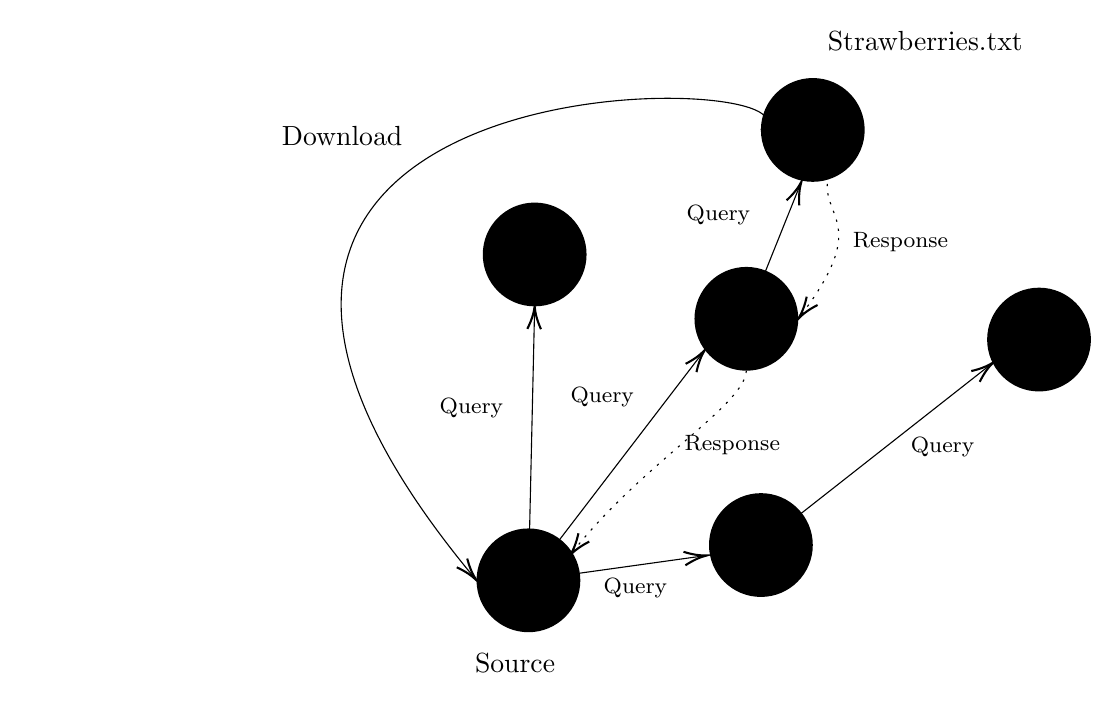
\begin{tikzpicture}[x=0.75pt,y=0.75pt,yscale=-1,xscale=1]
%uncomment if require: \path (0,451); %set diagram left start at 0, and has height of 451

%Shape: Circle [id:dp5701216218873355] 
\draw  [draw opacity=0][fill={rgb, 255:red, 0; green, 0; blue, 0 }  ,fill opacity=1 ] (100,126) .. controls (100,112.19) and (111.19,101) .. (125,101) .. controls (138.81,101) and (150,112.19) .. (150,126) .. controls (150,139.81) and (138.81,151) .. (125,151) .. controls (111.19,151) and (100,139.81) .. (100,126) -- cycle ;
%Shape: Circle [id:dp6701758191642804] 
\draw  [draw opacity=0][fill={rgb, 255:red, 0; green, 0; blue, 0 }  ,fill opacity=1 ] (202,157) .. controls (202,143.19) and (213.19,132) .. (227,132) .. controls (240.81,132) and (252,143.19) .. (252,157) .. controls (252,170.81) and (240.81,182) .. (227,182) .. controls (213.19,182) and (202,170.81) .. (202,157) -- cycle ;
%Shape: Circle [id:dp06164798754338219] 
\draw  [draw opacity=0][fill={rgb, 255:red, 0; green, 0; blue, 0 }  ,fill opacity=1 ] (209,266) .. controls (209,252.19) and (220.19,241) .. (234,241) .. controls (247.81,241) and (259,252.19) .. (259,266) .. controls (259,279.81) and (247.81,291) .. (234,291) .. controls (220.19,291) and (209,279.81) .. (209,266) -- cycle ;
%Shape: Circle [id:dp8491121482645921] 
\draw  [draw opacity=0][fill={rgb, 255:red, 0; green, 0; blue, 0 }  ,fill opacity=1 ] (97,283) .. controls (97,269.19) and (108.19,258) .. (122,258) .. controls (135.81,258) and (147,269.19) .. (147,283) .. controls (147,296.81) and (135.81,308) .. (122,308) .. controls (108.19,308) and (97,296.81) .. (97,283) -- cycle ;
%Shape: Circle [id:dp21625012916250363] 
\draw  [draw opacity=0][fill={rgb, 255:red, 0; green, 0; blue, 0 }  ,fill opacity=1 ] (343,167) .. controls (343,153.19) and (354.19,142) .. (368,142) .. controls (381.81,142) and (393,153.19) .. (393,167) .. controls (393,180.81) and (381.81,192) .. (368,192) .. controls (354.19,192) and (343,180.81) .. (343,167) -- cycle ;
%Shape: Circle [id:dp13339461282709586] 
\draw  [draw opacity=0][fill={rgb, 255:red, 0; green, 0; blue, 0 }  ,fill opacity=1 ] (234,66) .. controls (234,52.19) and (245.19,41) .. (259,41) .. controls (272.81,41) and (284,52.19) .. (284,66) .. controls (284,79.81) and (272.81,91) .. (259,91) .. controls (245.19,91) and (234,79.81) .. (234,66) -- cycle ;
%Straight Lines [id:da3027711082216963] 
\draw    (122,283) -- (124.95,153) ;
\draw [shift={(125,151)}, rotate = 91.3] [color={rgb, 255:red, 0; green, 0; blue, 0 }  ][line width=0.75]    (10.93,-3.29) .. controls (6.95,-1.4) and (3.31,-0.3) .. (0,0) .. controls (3.31,0.3) and (6.95,1.4) .. (10.93,3.29)   ;
%Straight Lines [id:da7950984523527296] 
\draw    (122,283) -- (205.78,173.59) ;
\draw [shift={(207,172)}, rotate = 127.44] [color={rgb, 255:red, 0; green, 0; blue, 0 }  ][line width=0.75]    (10.93,-3.29) .. controls (6.95,-1.4) and (3.31,-0.3) .. (0,0) .. controls (3.31,0.3) and (6.95,1.4) .. (10.93,3.29)   ;
%Straight Lines [id:da09130077482969812] 
\draw    (227,157) -- (252.75,92.86) ;
\draw [shift={(253.5,91)}, rotate = 111.88] [color={rgb, 255:red, 0; green, 0; blue, 0 }  ][line width=0.75]    (10.93,-3.29) .. controls (6.95,-1.4) and (3.31,-0.3) .. (0,0) .. controls (3.31,0.3) and (6.95,1.4) .. (10.93,3.29)   ;
%Straight Lines [id:da12456388559739229] 
\draw    (122,283) -- (206.02,271.28) ;
\draw [shift={(208,271)}, rotate = 172.06] [color={rgb, 255:red, 0; green, 0; blue, 0 }  ][line width=0.75]    (10.93,-3.29) .. controls (6.95,-1.4) and (3.31,-0.3) .. (0,0) .. controls (3.31,0.3) and (6.95,1.4) .. (10.93,3.29)   ;
%Straight Lines [id:da07990008290925488] 
\draw    (234,266) -- (344.43,179.24) ;
\draw [shift={(346,178)}, rotate = 141.84] [color={rgb, 255:red, 0; green, 0; blue, 0 }  ][line width=0.75]    (10.93,-3.29) .. controls (6.95,-1.4) and (3.31,-0.3) .. (0,0) .. controls (3.31,0.3) and (6.95,1.4) .. (10.93,3.29)   ;
%Curve Lines [id:da429610739418806] 
\draw  [dash pattern={on 0.84pt off 2.51pt}]  (266,92) .. controls (265.01,108.83) and (285.58,112.92) .. (253,155.69) ;
\draw [shift={(252,157)}, rotate = 307.69] [color={rgb, 255:red, 0; green, 0; blue, 0 }  ][line width=0.75]    (10.93,-3.29) .. controls (6.95,-1.4) and (3.31,-0.3) .. (0,0) .. controls (3.31,0.3) and (6.95,1.4) .. (10.93,3.29)   ;
%Curve Lines [id:da06143305048271208] 
\draw  [dash pattern={on 0.84pt off 2.51pt}]  (227,182) .. controls (226.01,198.83) and (177,226.44) .. (143.02,269.68) ;
\draw [shift={(142,271)}, rotate = 307.69] [color={rgb, 255:red, 0; green, 0; blue, 0 }  ][line width=0.75]    (10.93,-3.29) .. controls (6.95,-1.4) and (3.31,-0.3) .. (0,0) .. controls (3.31,0.3) and (6.95,1.4) .. (10.93,3.29)   ;
%Curve Lines [id:da928537814793256] 
\draw    (234,66) .. controls (274,36) and (-119,25) .. (97,283) ;
\draw [shift={(97,283)}, rotate = 230.06] [color={rgb, 255:red, 0; green, 0; blue, 0 }  ][line width=0.75]    (10.93,-3.29) .. controls (6.95,-1.4) and (3.31,-0.3) .. (0,0) .. controls (3.31,0.3) and (6.95,1.4) .. (10.93,3.29)   ;

% Text Node
\draw (265,17) node [anchor=north west][inner sep=0.75pt]   [align=left] {Strawberries.txt};
% Text Node
\draw (78,194) node [anchor=north west][inner sep=0.75pt]   [align=left] {{\footnotesize Query}};
% Text Node
\draw (141,189) node [anchor=north west][inner sep=0.75pt]   [align=left] {{\footnotesize Query}};
% Text Node
\draw (197,101) node [anchor=north west][inner sep=0.75pt]   [align=left] {{\footnotesize Query}};
% Text Node
\draw (305,213) node [anchor=north west][inner sep=0.75pt]   [align=left] {{\footnotesize Query}};
% Text Node
\draw (157,281) node [anchor=north west][inner sep=0.75pt]   [align=left] {{\footnotesize Query}};
% Text Node
\draw (277,114) node [anchor=north west][inner sep=0.75pt]   [align=left] {{\footnotesize Response}};
% Text Node
\draw (196,212) node [anchor=north west][inner sep=0.75pt]   [align=left] {{\footnotesize Response}};
% Text Node
\draw (95,317) node [anchor=north west][inner sep=0.75pt]   [align=left] {Source};
% Text Node
\draw (2,63) node [anchor=north west][inner sep=0.75pt]   [align=left] {Download};


\end{tikzpicture}

    \caption{Gnutella network example}
    \label{fig:gnutella}
\end{figure}

At its core, Gnutella is a protocol for search on a flat topology of nodes. Although files are stored in a centralised fashion, i.e.\ a node is responsible for storing a file not the entire network, Gnutella implements a decentralised model for document location and retrieval. Figure~\ref{fig:gnutella} shows the process of retrieving the \verb+Strawberries.txt+ file on a Gnutella network. In this model, every node is a server and a client; they can both query and deliver information. The network topology is flat and each node shares the same similar functionality, so they can be termed as `peers'.

On the Gnutella network there is no centralised directory and the system does not precisely control the network topology or file placement. The placement of data items is not based on any knowledge of the topology, as in a structured peer-to-peer design. To locate a data item, a node queries its neighbours, and gradually floods the network in a Breadth-first search manner. The lookup query is flooded to all neighbours, and if no match is found, the query is then forwarded to their neighbours. The query is typically bounded to a certain radius which is specified with a Time-to-Live (TTL) flag. This design is resilient to high churn rates, i.e., peers entering and leaving the system\cite{lua2005survey}. However, as the network grows, the search mechanisms do not scale effectively and generate unexpected loads on the network\cite{lua2005survey}.

To join the network, a node initially connects to one of several hosts that are known to be highly available, these are listed on the Gnutella website. This is one of the main weaknesses of the project. While the search mechanism is decentralised and is hence robust and fault-tolerant, the way of first joining and interacting with the network requires a form of centralisation. The ability for new nodes to join is entirely dependent on the availability of the known hosts listed on the Gnutella website. If the known hosts or the website itself were to become unavailable, then no new nodes would be able to join. Having nodes unable to join the network affects the overall probability of the network fulfilling its service.

Once connected to the network, peers can send messages to each other (refer to Figure~\ref{fig:gnutella}). These messages are either directly communicated to all peers with which the sender has open TCP connections or back-propagated, i.e., sent on a specific connection on the reverse of the path taken by an initial broadcast message. Each peer keeps a short cache of the recently routed messages in order to prevent re-broadcasting and to implement back-propagation.\cite{lua2005survey}

% Peers can send the following messages:
% \begin{itemize}
%     \item \textbf{Group Membership} - A peer joining the network broadcasts \verb+PING+ message to announce its presence. The message is then forwarded to its neighbours, initiating back-propagated \verb+PONG+ messages, which contains information about peers, such as the IP address, number and size of the data items.
%     \item \textbf{Search} - A \verb+QUERY+ contains a user specified search string that each receiving peer matches against locally stored file names. The \verb+QUERY+ is broadcasted. \verb+QUERY RESPONSE+ messages are back-propagated replies to \verb+QUERY+ messages and include information necessary to download a file.
%     \item \textbf{File Transfer} - File downloads are performed directly between two peers using these types of messages.
% \end{itemize}

To become a member of the network, a node has to open at least one connection with other peers already on the network. Peers periodically send \verb+PING+ messages to their neighbours to discover other participating peers. A peer decides who to connect to based only on local information. The entire application-level network is composed of peers and open TCP connections as links. The resulting network is a dynamic, self-organised network of independent entities.

Later versions of Gnutella introduced super-peers or ultra-peers\cite{rasti2005long}. These are self-appointed peers with better bandwidth connectivity. Requests are preferentially routed via super-peers, if possible, to help improve the routing performance of the network. However, the design is still limited by the fundamental need to flood large parts of the network to retrieve information.

Finally, while Gnutella laid some of the foundations for implementing a decentralised search mechanism, it does not provide means for improving information availability by having information maintained by the network rather than being strictly tied to a node.

% \cite{ripeanu2001peer} - This could be another good source


\section{JXTA}
\label{sec:jxta}

JXTA\cite{gong2001jxta} was initially released by Sun Microsystems in 2001. It is a network programming and computing platform that is designed to solve a number of problems in distributed computing, especially in peer-to-peer networking\cite{gong2001jxta}. The project was discontinued when Sun was acquired by Oracle in 2009. JXTA provided a network programming platform specifically designed to be the foundation for peer-to-peer systems. The resulting platform was independent of specific transport protocols, languages and application logic.

% \begin{itemize}
%     \item \textbf{Interoperability} - Many of the existing peer-to-peer systems at the time were stricly tied to the user-level application logic, e.g., Napster provided music file sharing and Gnutella provides generic file sharing. There was a lack of common underlying peer-to-peer infrastructure and the resulting systems were incompatible. This meant that existing peer-to-peer communities were duplicating efforts in creating software and system primitives commonly used by all peer-to-peer systems. ``Project JXTA aims to bring to the P2P world what HTTP and the browser brought to the Internet"\cite{jxta}
%     \item \textbf{Platform independence} - Many P2P systems offer their features or
% services through a set of APIs that are delivered on
% a particular operating system using a specific networking protocol. This requires the same system to be developed several times to service a wide peer-to-peer community. JXTA technology was designed to be independent of pre-
% ferred programming languages, development envi-
% ronments, or deployment platforms
%     \item \textbf{Ubiquity} - be implementable
% on every device with a digital heartbeat, including
% sensors, consumer electronics, PDAs, appliances,
% network routers, desktop computers, data-center
% servers, and storage systems
% \end{itemize}

\begin{figure}[ht]
    \centering
    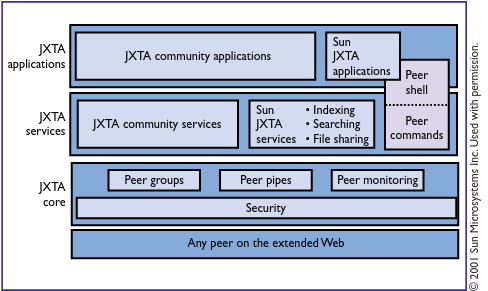
\includegraphics[width=0.7\textwidth]{imgs/Screenshot from 2022-04-16 09-32-03.png}
    \caption{P2P software architecture. JXTA technology provides a layer on top of which services and applications are built. \textit{credit: http://www.jxta.org}}
    \label{fig:jxta_architecture}
\end{figure}

Figure~\ref{fig:jxta_architecture} shows how the JXTA architecture stack breaks down into three layers. At the bottom, the core layer deals with peer establishment, communication management such as routing, and other low-level elements. The six protocols at the JXTA core are listed in Appendix~\ref{jxtaProtocols}. In the middle, a service layer handles higher-level concepts, such as searching and file sharing. The top layer is for application services such as messaging, and storage systems.

% https://ieeexplore.ieee.org/abstract/document/935182


\section{BitTorrent}
\label{sec:bittorrent}

BitTorrent\cite{cohen2008bittorrent} is a centralised peer-to-peer protocol that was originally conceived in 2001 by Bram Cohen. The protocol was designed to deliver a file sharing service similar to that of Gnutella. In BitTorrent, like in Gnutella, the burden of file storage is on the community, however, BitTorrent systems also have central serving nodes that handle location management. This enables much greater performance in information retrieval while maintaining some of the advantages of peer-to-peer architectures, namely, sharing bandwidth and load across the network and mitigating the need for data centres\cite{lua2005survey}.

The protocol is designed to incite contribution by taking a `tit-for-tat' approach where a peer responds with the same action that its other collaborating peer performed previously, e.g., if a node downloads a file hosted by other nodes, it subsequently hosts the file.

\begin{figure}[ht]
    \centering
    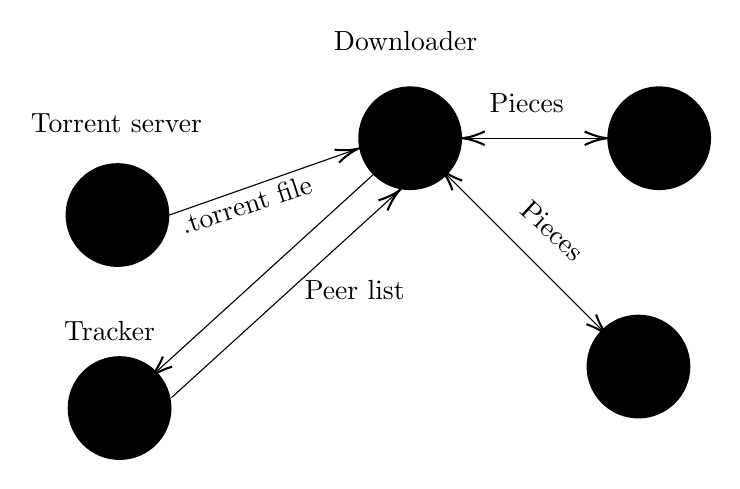
\begin{tikzpicture}[x=0.75pt,y=0.75pt,yscale=-1,xscale=1]
%uncomment if require: \path (0,300); %set diagram left start at 0, and has height of 300

%Shape: Circle [id:dp48020129375115905]
    \draw  [draw opacity=0][fill={rgb, 255:red, 0; green, 0; blue, 0 }  ,fill opacity=1 ] (290,195) .. controls (290,181.19) and (301.19,170) .. (315,170) .. controls (328.81,170) and (340,181.19) .. (340,195) .. controls (340,208.81) and (328.81,220) .. (315,220) .. controls (301.19,220) and (290,208.81) .. (290,195) -- cycle ;
%Shape: Circle [id:dp34478913628095786]
    \draw  [draw opacity=0][fill={rgb, 255:red, 0; green, 0; blue, 0 }  ,fill opacity=1 ] (289,102) .. controls (289,88.19) and (300.19,77) .. (314,77) .. controls (327.81,77) and (339,88.19) .. (339,102) .. controls (339,115.81) and (327.81,127) .. (314,127) .. controls (300.19,127) and (289,115.81) .. (289,102) -- cycle ;
%Shape: Circle [id:dp057127662756395914]
    \draw  [draw opacity=0][fill={rgb, 255:red, 0; green, 0; blue, 0 }  ,fill opacity=1 ] (430,65) .. controls (430,51.19) and (441.19,40) .. (455,40) .. controls (468.81,40) and (480,51.19) .. (480,65) .. controls (480,78.81) and (468.81,90) .. (455,90) .. controls (441.19,90) and (430,78.81) .. (430,65) -- cycle ;
%Shape: Circle [id:dp4152860206319915]
    \draw  [draw opacity=0][fill={rgb, 255:red, 0; green, 0; blue, 0 }  ,fill opacity=1 ] (550,65) .. controls (550,51.19) and (561.19,40) .. (575,40) .. controls (588.81,40) and (600,51.19) .. (600,65) .. controls (600,78.81) and (588.81,90) .. (575,90) .. controls (561.19,90) and (550,78.81) .. (550,65) -- cycle ;
%Shape: Circle [id:dp7865484354927322]
    \draw  [draw opacity=0][fill={rgb, 255:red, 0; green, 0; blue, 0 }  ,fill opacity=1 ] (540,175) .. controls (540,161.19) and (551.19,150) .. (565,150) .. controls (578.81,150) and (590,161.19) .. (590,175) .. controls (590,188.81) and (578.81,200) .. (565,200) .. controls (551.19,200) and (540,188.81) .. (540,175) -- cycle ;
%Straight Lines [id:da837231546510533]
    \draw    (339,102) -- (428.11,70.66) ;
    \draw [shift={(430,70)}, rotate = 160.63] [color={rgb, 255:red, 0; green, 0; blue, 0 }  ][line width=0.75]    (10.93,-3.29) .. controls (6.95,-1.4) and (3.31,-0.3) .. (0,0) .. controls (3.31,0.3) and (6.95,1.4) .. (10.93,3.29)   ;
%Straight Lines [id:da29190602799399223]
    \draw    (440,80) -- (331.48,178.65) ;
    \draw [shift={(330,180)}, rotate = 317.73] [color={rgb, 255:red, 0; green, 0; blue, 0 }  ][line width=0.75]    (10.93,-3.29) .. controls (6.95,-1.4) and (3.31,-0.3) .. (0,0) .. controls (3.31,0.3) and (6.95,1.4) .. (10.93,3.29)   ;
%Straight Lines [id:da7788788491503738]
    \draw    (340,190) -- (448.52,91.35) ;
    \draw [shift={(450,90)}, rotate = 137.73] [color={rgb, 255:red, 0; green, 0; blue, 0 }  ][line width=0.75]    (10.93,-3.29) .. controls (6.95,-1.4) and (3.31,-0.3) .. (0,0) .. controls (3.31,0.3) and (6.95,1.4) .. (10.93,3.29)   ;
%Straight Lines [id:da42573370946311306]
    \draw    (548,65) -- (482,65) ;
    \draw [shift={(480,65)}, rotate = 360] [color={rgb, 255:red, 0; green, 0; blue, 0 }  ][line width=0.75]    (10.93,-3.29) .. controls (6.95,-1.4) and (3.31,-0.3) .. (0,0) .. controls (3.31,0.3) and (6.95,1.4) .. (10.93,3.29)   ;
    \draw [shift={(550,65)}, rotate = 180] [color={rgb, 255:red, 0; green, 0; blue, 0 }  ][line width=0.75]    (10.93,-3.29) .. controls (6.95,-1.4) and (3.31,-0.3) .. (0,0) .. controls (3.31,0.3) and (6.95,1.4) .. (10.93,3.29)   ;
%Straight Lines [id:da47394536708390655]
    \draw    (548.59,158.59) -- (471.41,81.41) ;
    \draw [shift={(470,80)}, rotate = 45] [color={rgb, 255:red, 0; green, 0; blue, 0 }  ][line width=0.75]    (10.93,-3.29) .. controls (6.95,-1.4) and (3.31,-0.3) .. (0,0) .. controls (3.31,0.3) and (6.95,1.4) .. (10.93,3.29)   ;
    \draw [shift={(550,160)}, rotate = 225] [color={rgb, 255:red, 0; green, 0; blue, 0 }  ][line width=0.75]    (10.93,-3.29) .. controls (6.95,-1.4) and (3.31,-0.3) .. (0,0) .. controls (3.31,0.3) and (6.95,1.4) .. (10.93,3.29)   ;

% Text Node
    \draw (271,52) node [anchor=north west][inner sep=0.75pt]   [align=left] {Torrent server};
% Text Node
    \draw (287,152) node [anchor=north west][inner sep=0.75pt]   [align=left] {Tracker };
% Text Node
    \draw (417,12) node [anchor=north west][inner sep=0.75pt]   [align=left] {Downloader};
% Text Node
    \draw (341.71,101.92) node [anchor=north west][inner sep=0.75pt]  [rotate=-341.81] [align=left] {.torrent file};
% Text Node
    \draw (403,132) node [anchor=north west][inner sep=0.75pt]   [align=left] {Peer list};
% Text Node
    \draw (492,42) node [anchor=north west][inner sep=0.75pt]   [align=left] {Pieces};
% Text Node
    \draw (513.44,92.15) node [anchor=north west][inner sep=0.75pt]  [rotate=-42.84] [align=left] {Pieces};

\end{tikzpicture}


    \caption{BitTorrent architecture}
    \label{fig:bittorentArchitecture}
\end{figure}

The architecture (depicted in Figure~\ref{fig:bittorentArchitecture}) consists of a central location, called a tracker and many peers. When attempting to download a file from the network a peer initially connects to a known tracker to download a \verb+.torrent+ file. This file contains metadata about the requested file such as its length, name, hashing information and URL of a tracker.

Trackers keep track of all the peers hosting a file using a protocol layered on top of HTTP. A downloader sends information about the file it is downloading to the tracker. The tracker responds with a list of contact information about the peers that are downloading the same file. Downloaders then use this information to connect to each other. A downloader that has the complete file, known as a seed, must send out at least one complete copy of the original file. Each downloader announces to all of its peers which piece of information it has. When a peer finishes downloading a piece, it checks that the hash matches with that of the \verb+.torrent+ file, and announces that it has that piece to all of its peers. This verifies data integrity.

% \section{Beaker browser and Hypercore protocol}

% The Beaker browser is an experimental peer-to-peer web browser which runs a peer process in the background while using a Chromium based browser\cite{beaker}. This allows users to contribute to the network as they are browsing the internet which presents an interesting model of internet consumption and infrastructure. In addition, the browser allows users to publish websites and upload files directly from the browser so that they are available on the peer-to-peer network. The browser provides a high-level GUI enabling ease of use for new users to insight a greater community of users and hence peers.

% Beaker is built on top of the Hypercore protocol, a ``peer-to-peer data network built on Hypercore logs"\cite{hypercore} known as `hypercores'. Hypercore is the evolution of the Dat protocol\cite{ogden2017dat}. Hypercores are signed, append-only logs that can be thought of as a `lightweight' blockchain without the consensus algorithm. Append-only logs can be thought of as arrays in which the operations can only be \verb+get(index)+, \verb+push(data)+ and \verb+retrieve+ but where you can never overwrite pre-existing entries. Using append-only logs, Hypercore can easily generate compressed bitfields describing which portions of a log a peer hosts. This helps make the replication protocol light and efficient\cite{hypercore}.

% Hypercore allows efficient and quick distribution of the logs as each peer can choose to download only the section of the log they are interested in, without having to download everything from the beginning. However, while Hypercore could be a powerful approach to designing peer-to-peer systems it has seen fairly little use in its seven years of development.

% Briefly discuss the trees that they use with cryptography...


\section{libp2p}
\label{sec:libp2p}

\verb+libp2p+, unlike Gnutella or BitTorrent, does not deliver a specific user service but rather provides developers with a platform to build decentralised applications, much like JXTA. As of time of writing, it is used as the underlying peer-to-peer networking stack behind the IPFS project, Filecoin (a cryptocurrency based on sharing files) and the Ethereum cryptocurrency. \verb+libp2p+ is not a single library but rather a continuously maintained specification for the implementation of the peer-to-peer protocols. The project's ambition is to inform and make developing peer-to-peer applications significantly easier in an effort to increase their ubiquity\cite{dias2018IntroLibp2p}.

\begin{figure}[ht]
    \centering
    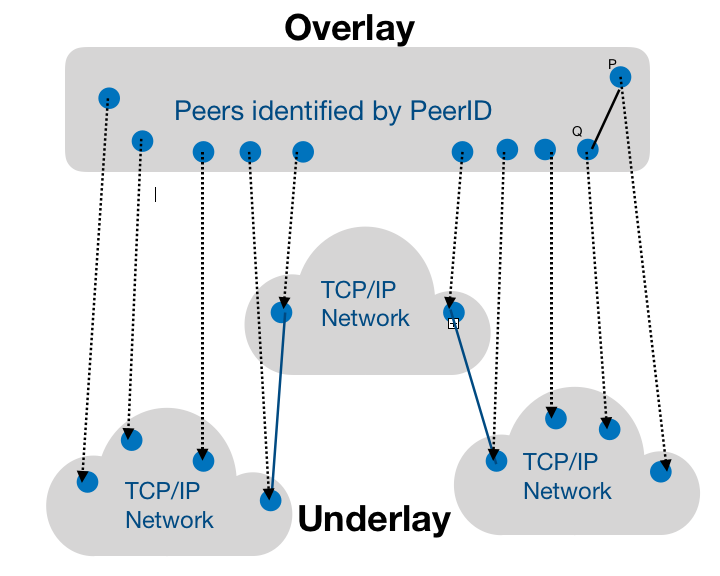
\includegraphics[width=0.5\textwidth]{imgs/0oGSfw7.png}
    \caption{libp2p Peer IDs that are unique across subnetworks}
    \label{fig:libp2pPeerIds}
\end{figure}

The project introduces some interesting innovations such as Peer IDs, which can uniquely identify peers across subnetworks producing an overlay that bridges networks (see Figure~\ref{fig:libp2pPeerIds}). One of the major innovation of \verb+libp2p+ is the introduction of `multiaddresses' which specify a peer and communication protocol in a standard string format. This allows the address to not only imply a recipient but also the protocol for addressing it. Peers can hence form connection between each other with many protocols for different scenarios. The connection between peers in \verb+libp2p+ is called a stream. More than one stream can be active between the same pair of peers, and each stream is logically independent of one another. When a new stream is opened, the two peers can negotiate which protocols should be used, and when a peer proposes a protocol to use, the other can accept it or send a message saying that it does not support it. When a consensus is reached, the peers will start using the agreed upon protocol.\cite{guidi2021libp2p}

To discover new peers in the network, \verb+libp2p+ uses multicast broadcasting for local peers and boostrap endpoints that enable the peer to be discovered by the wider network. When a peer is online, it can observe the network to learn which are the most reliable peers, i.e., highly available peers. By storing their IDs in a bootstrap list it can then readily join the network again without a prompted boostrap endpoint. Peers can share information about highly available nodes between themselves. This approach introduces some central points of failure in the discovery mechanisms, however, \verb+libp2p+ offers a fault-tolerant solution by providing several discovery mechanisms and relying on rendezvous as a fallback.

For NAT traversal \verb+libp2p+ offers several protocols. If the router supports UPnP (Universal Plug and Play) or nat-pmp (NAT Port Mapping Protocol), \verb+libp2p+ automatically tries to configure the router to enable inbound traffic. Another techniques used by \verb+libp2p+ is to listen to incoming connection on the same public port of the router as the port associated by the router to the peer's outbound connections. While these are far from perfect solutions, they are some of the best options currently available. NAT traversal could be avoided with wider adoption of the IPv6 protocol by Internet service providers (ISPs). IPv6 allows for the unique identification of all internet connected devices, but for the moment, most ISPs do not support the new protocol.

\verb+libp2p+ offers three protocols for content routing: Multicast DNS (mDNS), Kademlia DHT (KAD), and Publish-Subscribe. mDNS consists of broadcasting a query and asking local peers to identify themselves, while KAD leverages a Distributed Hash Table to find a peer with specific content. The Publish-Subscribe protocol has two implementations: FloodSub (based on network flooding) and GossipSub. In GossipSub peers are organised in a 2-layer logical network: a sparse layer, called full-message, where the published messages are exchanged using gossiping algorithms, and a dense layer, called metadata-only, used to maintain the other layer.\cite{guidi2021libp2p}

\begin{figure}[ht]
    \centering
    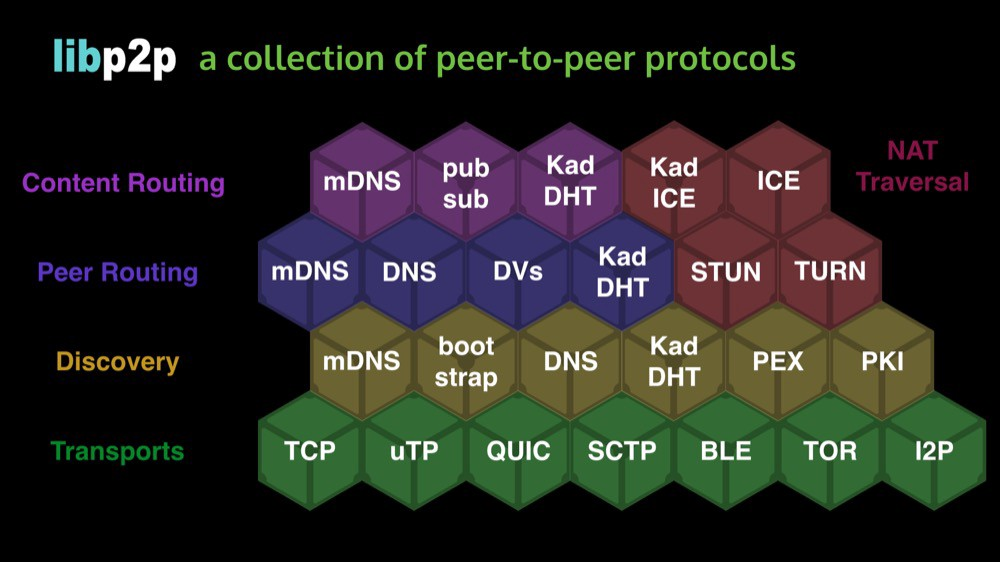
\includegraphics[width=0.7\textwidth]{imgs/libp2p.jpeg}
    \caption{libp2p modules}
    \label{fig:libp2pModules}
\end{figure}

One of the core characteristics of the \verb+libp2p+ project is that it is fundamentally modular this is expressed in their logo and is conveyed throughout their documentation. Each module can be imported separately and independently of any other module and addresses a specific problem in peer-to-peer distributed computing. The \verb+libp2p+ module architecture can be seen in Figure~\ref{fig:libp2pModules}.

    \chapter{Building Butter}
\label{ch:buildingButter}

In this chapter we cover the research and technical aspects of building the Butter framework. We shall discuss some general characteristics of the framework and global design decisions that have influence across all the modules. Then we shall dive into the specifics of each module, the problem(s) it seeks to solve, related work, design and implementation. We will then evaluate the module's design based on testing when appropriate.

Butter is a networking stack and framework for building decentralised applications (dapps). Hence, Butter's collection of modules can be used in conjunction to handle all the networking behaviour of a user specified decentralised application. Furthermore, the framework is designed to feel similar in use to other backend web development frameworks such as Django or Express. As a developer, you append extra functionality to a Butter node to describe the user-level application processing and the rest is handled by the framework. In other words, the framework's goal it to allow application services to be delivered, in a decentralised fashion, with minimum friction.

\begin{figure}[ht]
    \centering
    \documentclass{standalone}

\usepackage[most]{tcolorbox}
\usepackage{lmodern}
\usepackage{lipsum}
%\usepackage{geometry}

\standaloneenv{tcbposter}

%\pagestyle{empty}
\begin{document}

\begin{tcbposter}[
    poster = {columns=5, rows=7, width=9cm, height=6cm, spacing=1mm},% showframe},
    boxes = {
        boxrule=0pt, arc=2mm,
%        halign=center, valign=center,
        colupper=black,
        fontupper=\sffamily\bfseries, size=small}
]


\posterbox{column=1, row=1}{Discover}
\posterbox{column=2, row=1}{Traverse}
\posterbox{column=3, row=1}{Store}
\posterbox{column=4, row=1}{Retrieve}
\posterbox{column=5, row=1}{Butter application}
\posterbox{column=1, row=2, span=5}{Butter node}
\posterbox{column=1, row=3, span=5}{Session (Socket)}
\posterbox{column=1, row=4, span=5}{Transport (TCP)}
\posterbox{column=1, row=5, span=5}{Network (IPv4/IPv6)}
\posterbox{column=1, row=6, span=5}{Data link}
\posterbox{column=1, row=7, span=5}{Physical}

\end{tcbposter}

\end{document}

    \caption{Networking stack with Butter}
    \label{fig:butter-platform-taxonomy}
\end{figure}

Figure~\ref{fig:butter-platform-taxonomy} shows how the framework lies within the wider networking stack. The top layer is a user-defined application which interacts with the Butter modules. The architecture is similar to that of JXTA as seen in Figure~\ref{fig:jxta_architecture}. Butter provides a high-level API for developers to use, abstracting away the underlying behaviour that handles the distributed aspects of the system.

Like in the Gnutella implementation, Butter nodes perform tasks normally associated with both clients and servers. On one hand, they provide client-side interfaces through which users can query other nodes of the network, while at the same time they also accept queries from nodes and respond based on their partial view of the system. The decentralised design should result in highly fault-tolerant characteristics, as operation of the network will not be interrupted if a subset of nodes goes offline\cite{lua2005survey}.

Before covering the design specific to each module, we introduce the core design themes that run throughout the framework. These are listed bellow:

\begin{itemize}
    \item \textbf{Simplicity} - The framework should be simple to use and hence make building dapps easy. Interface should be designed in such as way as to make it feel similar to existing backend web frameworks in order make it familiar for developers and to minimise the learning curb.
    \item \textbf{Modularity} - A core theme of the framework is modularity, each module is independent and self-contained with consistent interfaces defined between the modules. Developers only need to import what they require. In addition, it allows developers to design their own module, specific to their needs and use them within Butter. This theme has another important justification, it allows us to experiment with different protocols implemented by various versions of a module.
    \item \textbf{Memory greedy} - This is a more difficult design theme to justify. When instantiating a Butter node, a user can specify how much memory to allocate to a node. The performance of the resulting network is greatly improved if nodes have a broader partial view of the network, so in general we tend to use as much memory as has been allocated favouring network performance over lower memory footprint.
    \item \textbf{Avoid panicking} - The network greatly benefits from having as many nodes as possible, maintaining nodes online in order to maximise data availability. Hence, we take a fault-tolerant approach to design where we prefer to manage faulty states rather than a fail-safe approach where we quickly resort to failing in order to minimise risk. We take a view that a node in a faulty state is still more valuable to the network than no node at all.
    \item \textbf{Diversity} - We want to accommodate all types of nodes and be flexible to different resources and device.
\end{itemize}

\begin{table}[ht]
    \center
    \begin{tabular}{|c|c|}
        \hline
        \textbf{Module}            & \textbf{Core technology}       \\
        \hline
        Discovery                  & UDP Multicast                  \\
        Known host management      & Known host quality metric      \\
        Wider discovery            & Port forwarding \& Ambassadors \\
        Persistent storage         & PCG                            \\
        Information retrieval (IR) & Random TTL BFS                 \\
        \hline
    \end{tabular}
    \caption{Summarising table of Butter modules and the core technology used to implement the solution}
    \label{tab:butterModules}
\end{table}

Table~\ref{tab:butterModules} can be used as a quick reference summarising the core technologies used in each module. Greater detail is provided in each of the module sections.

Finally, in order to reason about the module designs, we should stress the importance of message complexity in distributed system. As computer scientists we are used to seeing time and space complexity when assessing the theoretical efficiency of a design, however, in distributed systems there is an extra factor to take into account: message complexity. In the literature, message and communication complexity are used interchangeably to denote the amount of communications required to solve a problem when the input to the problem is distributed among two or more parties, graphically it can be expressed as the maximum number of messages transmitted over any edge\cite{yao2009communication}.

    \newpage
\section{Testbed}
\label{sec:testbed}

Butter provides a testbed that enables stress testing and experimenting with Butter peer-to-peer networks. The tool can be used to spawn $n$ nodes on a single machine (using go-routines), it can artificially introduce churn and add random data to the network. These steps can be carried out in various user defined sequences with timeouts allowing network recovery. Specific features of the tested can be extended based on the testing requirements of the module.

\subsection{Limitations \& challenges}

Firstly, it is important to note how difficult it is to accurately test peer-to-peer networks in simulation\cite{almeida2008framework}. The systems are designed to connect different remote devices and hence without access to large amounts of network testing hardware, it can be difficult to run accurate simulations. Simulating nodes on a single system will often be limited, despite efforts to add randomised latency and introduce node and link failure. While the simulation might not present a realistic environment it does give an opportunity to create extreme scenarios to test edge cases.

% In the simulated environment links are significantly faster and more stable than on a `real world' network. A representative test rig is difficult to achieve and the simulated environment is unlikely to reflect how nodes may behave on the wider internet.

In addition, there are hardware constraints to testing on a single system. Generating a large simulated network across many threads, introducing churn, and opening and closing ports in rapid succession locally on the system can cause the testbed to behave unpredictably. Hence, we are bounded on the amount of nodes that can be spawned by the test device's resources.

Nodes behave asynchronously so can take unpredictable amounts of time to spawn (e.g. blocking while OS allocates port or as thread gets created), and it is difficult to determine how long a spawned node will take to discover other nodes on the network. This means it is difficult to create and destroy nodes in rapid succession. We are forced to include timeouts to give nodes sufficient time to start up and connect to the network (i.e. discover other nodes). This results in unpredictable success of test runs and/or very long test runs (up to several hours).

An interesting future improvement to the testbed would be to allow the generation of specified network topologies\cite{zeinalipour2005peerware}. This would enable controlled tests of very specific edge cases.
    \newpage


\section{Discovery}
\label{sec:discovery}

% \subsection{Problem statement}

Before any service can be delivered by a node, it needs to be known by other nodes, i.e., a node cannot benefit from or provide a service to the network if it is unknown by the network. In an effort to remove any form of centralisation, nodes cannot communicate with a known endpoint at spawn because there is no known endpoint. In other words, when the node is first spawned, it is not aware of any other nodes and hence cannot participate in the network, so the problem can be thought of as: how does a node get known by other nodes and conversely how do other nodes get to know the newly spawned node?

Note that this version of the peer discovery problem is only relevant in local area networks (LAN). Local area networks generally provide highly reliable communication facilities based on broadcasting, making it much easier to develop distributed discovery systems\cite{tanenbaum2007distributed}. Please refer to the Wider discovery section to see how nodes discover each other across subnetworks.

\subsection{Related work}
Here we will discuss some notable mechanisms and technologies used to enable communication between initially unknown nodes on LAN.

\subsubsection{Broadcasting}

There are two types of network links: point-to-point links and broadcast links. A point-to-point link consists of a single `sender' process communicating with a single `receiving' process (often referred to as a listening process). Broadcast links, on the other hand, can have multiple sending and receiving nodes, all connected to the same shared broadcast channel\cite{kurose2010computer}. In essence, broadcasting allows all host connected to a network, to share the same communication channel and so a packet sent by a host is received by all the other hosts on the network.

In broadcasting, we often specify the address of the intended recipient in the address field of the packet. While the packet is sent to all others on the network, only the recipient host processes it. However, there is also a possibility to address a packet to all hosts on the network by specifying a special code in the address field of the packet. When the packet is transmitted, it is received and processed by all the host in the network.\cite{tenanbaum2012networks}

One of the main limitations of broadcast is that it has no mechanism to limit the recipients of a broadcast and so sends packets to all devices on a local area network. This is not of much importance on small local networks but can introduce significant bandwidth usage on larger LANs.

% Various methods have been proposed for Broadcasting. One such method that requires no special features from the network is for the source to send a distinct packet to each destination. Not only is the method wasteful of bandwidth and slow, but it also requires the source to have a complete list of all destinations. This method is not desirable in practice, even though it is widely applicable.\cite{tenanbaum2012}

% Another more elegant solution to broadcasting is the method of reverse path forwarding\cite{dalal1978reverse}. When a broadcast packet arrives at a router, the router checks to see if the packet arrived on the link that is normally used for sending packets toward the source of the broadcast. If so, there is an excellent chance that the broadcast packet itself followed the best route from the router and is therefore the first copy to arrive at the router. This being the case, the router forwards copies of it onto all links except the one it arrived on. If, however, the broadcast packet arrived on a link other than the preferred one for reaching the source, the packet is discarded as a likely duplicate.\cite{tenanbaum2012}

\subsubsection{Multicasting}

Multicasting is a transmission method in which copies of a packet are transmitted to a group of the hosts in the network interested in receiving the packet. The relationship between source and destination is one-to-many, as apposed to one-to-all for broadcasting. In multicasting, destination address is specified as a group address.

Multicast group membership is configured when devices send `join' packets to an upstream router. The routers and switches keep track of this membership; so when multicast packets arrive at a switch, they are only sent to devices that want them.

\subsubsection{Multicast DNS}

Multicast DNS (mDNS) is a technology originally developed at Apple under the name Bonjour and has since been adopted as an internet standard\cite{cheshire2013mdns}. It is used to locate a device or service by name on a small local network without using a pre-configured name sever, i.e, a DNS. While the protocol uses the same packet structure and commands as DNS, it does not rely on a DNS server, instead computers on a network create their own local DNS records and store them in memory. When a host on the network requires the IP address of another host, it sent a DNS query using a multicast UDP message. All mDNS hosts see this query and the host storing the IP address responds. Because messages are exchanged using multicast, all other mDNS hosts see this exchange and can make a note of the network name and IP address. They can then update their local cache.

\subsection{Design \& implementation}

The Butter Peer discovery mechanism is loosely inspired by the mDNS protocol. Multicast was preferred over broadcast in an effort to minimise wasted bandwidth usage. With multicast only devices running Butter node processes, receive and interpret packages.

As a node spawns, it initially has no known hosts. When a node's list of known hosts is empty, the node goes into discovery mode. In discovery mode, the node, at regular intervals, sends a $PING$ packet containing its listening address along a UDP multicast channel. All peers have a background procedure that listens out for incoming $PING$ packets. If a $PING$ packet is received by a remote host, it attempts to append the new host to its list of known hosts (given enough available memory) and responds with a $PONG$ packet containing its own listening address. If a discovering node receives no response, a 10-second timeout occurs before trying again.

Please see Algorithms~\ref{alg:ping} and~\ref{alg:pong} to view the pseudocode for the discovery mechanism.

\begin{algorithm}
    \While{no known hosts}{
        Send ping message long a UDP multicast channel\;
        Wait up to 10 seconds for a response\;
        \eIf{$response \neq \emptyset$}{
            Append payload (remote node's listening address) to local list of known hosts\;
            \Break\;
        }{
            Timeout for 10 seconds\;
        }
    }
    \caption{Procedure for pinging out to other nodes}
    \label{alg:ping}
\end{algorithm}

\begin{algorithm}
    \While{}{
        Listen for broadcast packets in the multicast channel\;
        \If {$packet \neq \emptyset \And packetType = PING$} {
            Try to append to local list of known hosts\;
            Send a response containing address\;
        }
    }
    \caption{Procedure for listening out to ping requests to join the network}
    \label{alg:pong}
\end{algorithm}

%In Algorithm~\reg{algo:ping}, we are forced to have an upper bound timout while waiting for a response as we are operating under an asynchronous network model. That is, there is no upper bound on the amount of a time a message might take to be transmitted on the network

This implementation uses Go routines, which are lightweight threads to run the asynchronous procedures. In addition, Go provides in its default \verb+net+ packages an implementation of a UDP multicasting server and client which is used to initialise the UDP multicast channel.

Once an initial connection is made, the $PING$ procedure stops and will only restart if the node detects it no longer has any known hosts. Nodes will always be listening out for incoming $PING$ packets. Once connected a node can learn about other peers on the network by querying its newly known host about the other remote hosts.

\subsection{Testing \& Evaluation}

The approach taken by Butter is similar to that of \verb+libp2p+ when discovering local peers. While it is effective, and uses significantly less bandwidth than broadcasting, there are some limitations. Firstly, the ping timeout interval affects the speed at which a new node can be discovered by the network. In worst case, discovery can be as long as the peer timeout interval plus any latency.

In a simulated testing environment, using the Butter testbed, a slow ping rate affected network functionality as nodes programmatically attempted to retrieve information before having any known hosts. In a practical environment this should not pose an issue but the module does provide a user parameter to change the default 10 second interval, so it can be best set to suit the operating environment. In most practical cases, a 10 second interval should suffice.

Finally, as discussed previously, the main limitation of this method is that it is restricted to LAN discovery. In addition, on certain LAN networks with extra security protocols, UPD multicasting to certain reserved groups may fail and hence nodes will be unable to discover each other. A solution to this may be to implement several fall-back discovery protocols like in \verb+libp2p+, this could be developed in later version of the project.
    \newpage


\section{Known host management}
\label{sec:knownHostManagement}

% Problem statement
Known host management in an unstructured peer-to-peer system is arguably simpler than in a structured peer-to-peer architecture. Graphically, if a node is a vertex, its known hosts determines its edges. The direction of the edges imply `who knows who', i.e., if nodes are known to each other, the edge is bidirectional. It is also possible that the hosts are not mutually known to each other.

In a structured network, a certain topology needs to be maintained in order for the overlay network to behave as intended\cite{stoica2003chord}. In an unstructured topology, there is no need to maintain known hosts in a specific structure, however, maintaining a balance between the amount of known hosts so that the network is sufficiently connected to function effectively, but not too many as to exceed a node's resources, is important\cite{lua2005survey}. Node's have finite memory to store known hosts so peer selection becomes important.

\begin{figure}[ht]
    \centering
    
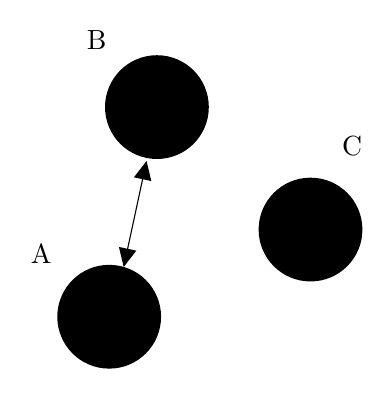
\begin{tikzpicture}[x=0.75pt,y=0.75pt,yscale=-1,xscale=1]
%uncomment if require: \path (0,300); %set diagram left start at 0, and has height of 300

%Shape: Circle [id:dp1418814839562289] 
\draw  [draw opacity=0][fill={rgb, 255:red, 0; green, 0; blue, 0 }  ,fill opacity=1 ] (116,196) .. controls (116,182.19) and (127.19,171) .. (141,171) .. controls (154.81,171) and (166,182.19) .. (166,196) .. controls (166,209.81) and (154.81,221) .. (141,221) .. controls (127.19,221) and (116,209.81) .. (116,196) -- cycle ;
%Shape: Circle [id:dp3981484481701938] 
\draw  [draw opacity=0][fill={rgb, 255:red, 0; green, 0; blue, 0 }  ,fill opacity=1 ] (139,95) .. controls (139,81.19) and (150.19,70) .. (164,70) .. controls (177.81,70) and (189,81.19) .. (189,95) .. controls (189,108.81) and (177.81,120) .. (164,120) .. controls (150.19,120) and (139,108.81) .. (139,95) -- cycle ;
%Shape: Circle [id:dp7390139799048381] 
\draw  [draw opacity=0][fill={rgb, 255:red, 0; green, 0; blue, 0 }  ,fill opacity=1 ] (213,154) .. controls (213,140.19) and (224.19,129) .. (238,129) .. controls (251.81,129) and (263,140.19) .. (263,154) .. controls (263,167.81) and (251.81,179) .. (238,179) .. controls (224.19,179) and (213,167.81) .. (213,154) -- cycle ;
%Straight Lines [id:da4506323249212101] 
\draw    (158.37,123.93) -- (148.63,169.07) ;
\draw [shift={(148,172)}, rotate = 282.17] [fill={rgb, 255:red, 0; green, 0; blue, 0 }  ][line width=0.08]  [draw opacity=0] (8.93,-4.29) -- (0,0) -- (8.93,4.29) -- cycle    ;
\draw [shift={(159,121)}, rotate = 102.17] [fill={rgb, 255:red, 0; green, 0; blue, 0 }  ][line width=0.08]  [draw opacity=0] (8.93,-4.29) -- (0,0) -- (8.93,4.29) -- cycle    ;

% Text Node
\draw (102,160) node [anchor=north west][inner sep=0.75pt]   [align=left] {A};
% Text Node
\draw (129,57) node [anchor=north west][inner sep=0.75pt]   [align=left] {B};
% Text Node
\draw (252,108) node [anchor=north west][inner sep=0.75pt]   [align=left] {C};


\end{tikzpicture}
    \caption{Three severely memory restricted nodes with no form of known host management}
    \label{fig:memoryRestrictedUnmanaged}
\end{figure}

\begin{figure}[ht]
    \centering
    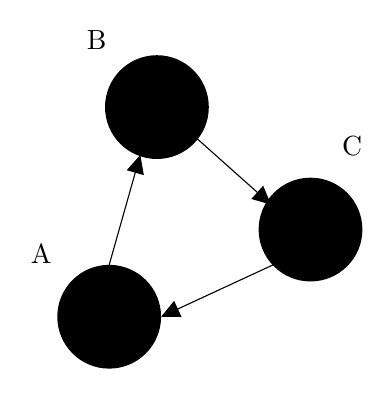
\begin{tikzpicture}[x=0.75pt,y=0.75pt,yscale=-1,xscale=1]
%uncomment if require: \path (0,300); %set diagram left start at 0, and has height of 300

%Shape: Circle [id:dp1418814839562289] 
\draw  [draw opacity=0][fill={rgb, 255:red, 0; green, 0; blue, 0 }  ,fill opacity=1 ] (116,196) .. controls (116,182.19) and (127.19,171) .. (141,171) .. controls (154.81,171) and (166,182.19) .. (166,196) .. controls (166,209.81) and (154.81,221) .. (141,221) .. controls (127.19,221) and (116,209.81) .. (116,196) -- cycle ;
%Shape: Circle [id:dp3981484481701938] 
\draw  [draw opacity=0][fill={rgb, 255:red, 0; green, 0; blue, 0 }  ,fill opacity=1 ] (139,95) .. controls (139,81.19) and (150.19,70) .. (164,70) .. controls (177.81,70) and (189,81.19) .. (189,95) .. controls (189,108.81) and (177.81,120) .. (164,120) .. controls (150.19,120) and (139,108.81) .. (139,95) -- cycle ;
%Shape: Circle [id:dp7390139799048381] 
\draw  [draw opacity=0][fill={rgb, 255:red, 0; green, 0; blue, 0 }  ,fill opacity=1 ] (213,154) .. controls (213,140.19) and (224.19,129) .. (238,129) .. controls (251.81,129) and (263,140.19) .. (263,154) .. controls (263,167.81) and (251.81,179) .. (238,179) .. controls (224.19,179) and (213,167.81) .. (213,154) -- cycle ;
%Straight Lines [id:da8506068290592598] 
\draw    (141,171) -- (155.18,120.89) ;
\draw [shift={(156,118)}, rotate = 105.8] [fill={rgb, 255:red, 0; green, 0; blue, 0 }  ][line width=0.08]  [draw opacity=0] (8.93,-4.29) -- (0,0) -- (8.93,4.29) -- cycle    ;
%Straight Lines [id:da3809501315965952] 
\draw    (182,109) -- (216.76,140) ;
\draw [shift={(219,142)}, rotate = 221.73] [fill={rgb, 255:red, 0; green, 0; blue, 0 }  ][line width=0.08]  [draw opacity=0] (8.93,-4.29) -- (0,0) -- (8.93,4.29) -- cycle    ;
%Straight Lines [id:da7416029981434609] 
\draw    (220,171) -- (168.72,194.74) ;
\draw [shift={(166,196)}, rotate = 335.16] [fill={rgb, 255:red, 0; green, 0; blue, 0 }  ][line width=0.08]  [draw opacity=0] (8.93,-4.29) -- (0,0) -- (8.93,4.29) -- cycle    ;

% Text Node
\draw (102,160) node [anchor=north west][inner sep=0.75pt]   [align=left] {A};
% Text Node
\draw (129,57) node [anchor=north west][inner sep=0.75pt]   [align=left] {B};
% Text Node
\draw (252,108) node [anchor=north west][inner sep=0.75pt]   [align=left] {C};


\end{tikzpicture}

    \caption{Three severely memory restricted nodes with known host management mechanism}
    \label{fig:memoryRestrictedManaged}
\end{figure}

One option is to simply choose known hosts on a `first-come-first-serve' basis, however, this causes issues in some cases. For example, take three severely memory restricted nodes that only have the capacity to store one known host each. Upon spawning, the first two would become aware of each other and hence store each other in their known host list, leaving the last node unknown and hence unable to participate in the network (illustrated in Figure~\ref{fig:memoryRestrictedUnmanaged}). This edge case highlights that we want to design a known host selection and maintenance protocol that, in addition to maintaining a list of alive known hosts, always accepts known hosts that would otherwise be unknown by the network (illustrated in Figure~\ref{fig:memoryRestrictedManaged}).

A few extra properties of known hosts might be desirable, for example, it might be easier to query large parts of the network if node $q$'s known hosts know a lot of other hosts. Furthermore, $q$ may want to have known hosts it can rely on, hence highly available. Finally, it might also be good to known hosts with lots of available storage so that $q$ can readily share information with its peers. Intuitively, we might be inclined to think that we should optimise known hosts to be highly available nodes, with plenty of available storage, that know lots of other nodes. However, if that were the case, new nodes would be actively disregarded by the network as they would inherently have low uptime and know relatively few other nodes. We have to make the distinction between what is good for the node and what is good for the network.

\subsection{Related work}

\subsubsection{Gnutella group membership messages}

While the Gnutella project does not implement a very complex known host management protocol it does implement a Group membership protocol in which a peer joining the network broadcasts $PING$ messages to announce its presence. The message is then forwarded to its neighbours, initiating back-propagated $PONG$ messages, which contain information about peers, such as the IP address, number and size of the data items.\cite{lua2005survey}

\subsubsection{JXTA peer information protocol}

Much like Gnutella, JXTA does not attempt to actively optimise a node's known hosts but provides a peer information protocol for peers to learn about the capabilities and status of others. For example, a $PING$ message can be sent to see if a peer is alive. A query can also be sent regarding a peer’s properties where each property is returned as a name and a value string.

\subsection{Design \& implementation}

In Butter, a node can query other remote nodes to obtain their $NodeQuality$ metadata. The data contained in $NodeQuality$ is: uptime, available storage space and number of known hosts. Nodes periodically request the $NodeQuality$ metrics from their known hosts and cache the data between updates.

% As an added optimisation, a node caches data when it updates its index of known host quality metric so as not to have to query its known hosts multiple times for many consecutive possible new host insertion

\subsubsection{Known host list maintenance}

Firstly, the simpler part of the Known host management module is handling dead known hosts. During the regular $NodeQuality$ requests, if a node is unresponsive, after a given timeout period, the host is removed from the list of known hosts. This reduces the probability that a node attempts to communicate with a dead host during other operations such as retrieving information or sharing discovered peers. Making sure that the hosts within the list are alive and responding with a minimum delay also prevents dead hosts from taking up list capacity, leaving room for new hosts to join.

\subsubsection{Peer selection}

In addition, the Known host management module is responsible for peer selection. Peer selection becomes a problem when a node's known host list is at capacity and hence decisions need to be made as whether knowing or ignoring a host is best (with regards to the node and the network).

The approach for designing peer selection is loosely inspired by various optimisation algorithms (optimal, sub-optimal and soft constraint). We define an optimisation problem to be: ``a set of variables, each with an associated domain, an objective function that maps total assignments to real numbers, and an optimality criterion, which is typically to find a total assignment that minimises or maximises the objective function"\cite{poole2017ai}. To avoid the edge case discussed previously, i.e., new peers being unable to get themselves known by pre-existing nodes on the network as they do not fit the desired $NodeQuality$, each node attempts to optimise its list of known hosts for a diverse distribution of $NodeQuality$s. In other words, nodes do not optimise for a specific kind of remote host but rather a diverse set of hosts. To put it in terms of an optimisation problem, the possible known hosts is the set of variables, each with an associated $NodeQuality$, the objective function determines how diverse the a known host list is (based on the node's own perception of diversity guided by its partial view) and the optimality criterion is to find a set of known host that maximises the node's known host diversity.\\

\noindent The procedure is as follow:
\begin{itemize}
    \item Trivially, if a node has sufficient memory to store a host, and does not already know it, store it (greedy philosophy)
    \item If the node is at capacity, determine, based on the characteristics of the node and those of its previously known hosts, whether the new host would make the list of known hosts more diverse
    \begin{itemize}
        \item If it does, remove a host from the most popular class of known host types and store the new one
        \item Else, do nothing
    \end{itemize}
\end{itemize}

Notice that this algorithm is somewhat reminiscent of the AI optimisation algorithms where given a current known host list state, we evaluate a permutations and consider whether the new states is an improvement or not.

The objective function for diversity is based on the node's partial view. A node looks at its metadata and the metadata of all of its immediate known hosts and classifies them according to this understanding of the network. With this objective function, at capacity, a node will attempt to have an equal distribution of node types, i.e., with varying $NodeQuality$ metrics, by mostly accepting nodes that increase the diversity of its list of known hosts.

% THIS IS VERY IMPORTANT - answers Nathan's question
An important edge case to consider is when many nodes are spawned in quick succession, with similar parameter settings, e.g., similar user allocated memory. This leads to many nodes with very similar $NodeQuality$ values. In this case, any given node will be optimising for a diverse set of known hosts, but the diversity between nodes and hence the global diversity may be poor. This results in the network converging towards knowing the same hosts. This can be thought of in terms of local and global diversity. % giving rise to the notion of internal (local) diversity and external (global) diversity.

In this scenario, all nodes have similar uptime, available storage and number known hosts, and hence have the same diversity metric. If a new node wants to joins the network, it runs through the Discovery protocol (as it knows no hosts) and is quickly accepted by a host (as hosts always accept nodes with no known hosts). However, if the node does not fit within the unanimous diversity metric it will quickly be rejected by the network, it will then go back into discovery mode, be discovered and eventually rejected once again. This will keep re-occurring.

A solution would be to not have any form of diversity driven optimisation and simply accept nodes at random, however, this may lead to uneven distribution of information on the network and poor network performance. Instead, we rely on a few factors to decrease the probability of this occurring. Firstly, in most practical environments nodes are not symmetric, nodes typically have their own very unique perception of the world as they have their own uptime, available storage (user allocated memory) and collection of known hosts. In addition a randomness factor is added to the diversity protocol. This means that on occasion a node is accepted or removed by chance despite its valuation by the objective function, i.e., regardless of the diversity metric. This prevents a convergence towards only accepting certain node types in an attempt to improve the probability of global diversity.

% In addition, It is worth noting that the probability of this edge case occurring in practice is somewhat mitigate by the fact that it is uncommon that many hosts all spawn at the same time (unless in simulated testing environments) and even more unlikely that nodes are symmetrical i.e. have exactly the same user specified allocated memory and hence the same amount of known hosts and available storage. By relying on the practical asymmetry between nodes and the added random acceptance we can mitigate the risk of a homogeneous global diversity. Known hosts are not symmetrical each is unique in the sense it has properties such as available memory, different uptime different set of known hosts - this means each node has a unique notion of what diverse based on its experience - this results in the overall network being diverse

\subsection{Testing \& evaluation}

% TODO: Get some hard numbers in for this somehow. e.g. in a a randomised network what is the diversity of peers? The NetworkX Python library might be a good fit

% \subsubsection{Known host list maintenance}

An extra optimisation to improve known host list maintenance would be to remove hosts that are found dead when carrying out other operations such as information retrieval. This would allow the list of known host to be updated between $NodeQuality$ request intervals. To achieve this we would have to introduce an API endpoint within the Known host management module to enable other modules to make changes to the known host list. However, this has the potential to increase complexity for developers and increases the risk of accidental mismanagement and incorrect removal of known hosts, so this feature is not implemented in the current version of the module.

During the implementation several different $NodeQuality$ intervals were explored. Obviously, short intervals means that the known host list is a better representation of the known hosts, however, this leads to greater message complexity. The message complexity of the $NodeQuality$ procedure grows linearly for a node based on the number of known hosts. On the other hand, the queries are exponential on a network level, as each node is querying its known hosts. The $NodeQuality$ interval should be a balance between maintaining an accurate reflection of the hosts and minimising network flooding.

% Maybe we should really be looking at Uptime or Storgae or Known host count and not the host class, as the classes are not comparable between nodes (each node has its own personal definition for a host type class.

\begin{table}[h]
    \centering
    \begin{tabular}{|l|c|c|c|}
        \hline
        \textbf{Test} & \textbf{S.D. Node A} & \textbf{S.D. Node B} & \textbf{Z-statistic} \\
        \hline
        No randomised acceptance, uniform nodes &  1.0897 & 0.9682 & 0.4797 \\
        Random acceptance, uniform nodes & 0.6614 & 0.9682 & 0.8472 \\
        Asymmetric nodes & 0.9990 &  0.8291 & 1.0640 \\
        \hline
    \end{tabular}
    \caption{Standard deviation of node types in three different test cases for two nodes chosen at random. Z-statistic is provided to compare distribution across the nodes.}
    \label{tab:diversityData}
\end{table}

% TODO: Remove the z stat because it is meaningless
In order to test the diversity mechanisms we generated several networks of Butter nodes at random using the testbed. The data from this experiment can be found in Table~\ref{tab:diversityData}. The standard deviation is a measure of distribution of host types. If the standard deviation is small, then we roughly have the same amount of each host type and the local diversity is relatively high. The $z$-statistic measure is used to compare the distribution between nodes.

% a low z-stat measure shows that the known hist list are similarly diverse across nodes

In the first instance of the test, nodes were spawned with the same allocated memory in quick succession, resulting in what we would assume to be similar host types. The mechanism that occasionally accepts a node at random regardless of host type was disabled. In this test, we observed slightly higher standard deviations of the host type distribution in comparisons to the other test environments. This suggests in a network with many uniform nodes, maintaining a diverse set of known hosts is more difficult. Note, that in all three testes, the difference in distribution of known hosts between the two nodes selected at random is fairly small suggesting there us little difference between the two distribution diversities. Once we introduce, the random acceptance mechanism, the standard deviation decreases suggesting there is greater diversity in the maintained list of known hosts.

In future it may be interesting to test how the network diversity mechanisms perform in prescribed topologies. Integrating the Butter testbed with tools such as NetworkX\cite{networkx2022networx, orda2019efficient} may allows the exploration of edge cases and provide a visual testing environment.

A last factor to consider is that $NodeQuality$ information becomes more quickly out-of-date on higher churn networks. If nodes are frequently dying and the interval is large, there is a higher probability that hosts in the list are unavailable. Currently the $NodeQuality$ update interval is a parameter that is user-specified. In a high-churn simulated environment (see Section~\ref{sec:churnTesting}) we saw significantly fewer failed requests when the update interval was 10 seconds as apposed to 30 seconds. An interesting future improvement might be to implement a dynamic update interval relying on some churn rate detection mechanism.

% \subsubsection{Peer selection}

% Another interesting parameter that can be changed is the frequency of accepting a new node at random and removing a node at random despite the objective function.

% Using the testing framework described in Section \ref{sec:testingMethodology} we compared the performance of information retrieval and persistent information storage on both unmanaged known hosts and managed known hosts. It was clear that 

Finally, in future, more metadata could be added to the $NodeQuality$ to broaden the diversity metric. For example, it may be interesting to give a sense of the information hosted by a peer, as having diverse knowledge between known hosts may increase the probability of quickly finding some piece of information.

    \newpage


\section{Wider discovery}
\label{sec:widerdiscovery}

% Problem statement
For peers to communicate over the internet they need to be accessible publicly, so that others can query them, i.e.\ so that they can serve requests. Once available publicly, they also need to be known by other peers on different subnetworks. This module was designed to address both those problems, referred to here as NAT traversal and Internet discovery respectively.

\subsubsection{NAT}

Network Address Translation (NAT) is the process of translating an IP address so that it makes sense from one subnetwork to another. It is necessary, as there are not enough addresses, when using IPv4, to uniquely identify every device on a large network. Instead, devices on a subnetwork lie behind a router which acts as an endpoint, routing packets to the appropriate device on the local area network. This solution makes it difficult for peers to `listen' to incoming connections behind a router.

When making a request a temporary port is opened in the router enabling the server to communicate with the device making the request. However, if a peer wishes to communicate with a peer on another subnetwork, i.e.\ it wishes to be served by another peer, it cannot uniquely identify that node as all it knows is the IP address of the subnetwork (i.e.\ that of the router), not that of the individual machine that could serve the request. A solution to this is provided by the IPv6 protocol, which introduces a significantly larger namespace, enabling unique identification of all internet connected devices. However, for security reasons many Internet Service Providers have not enabled IPv6 and hence the technology is not yet ubiquitous. The process of establishing and maintaining connections across gateways that implement network address translation is called NAT traversal, and it is requirement for peers to be able to serve each other.

% This is necessary as to efficiently use IP addresses they need to be allocated dynamically. IPv4 was conceived before the internet grew to the extent it is now. There are not sufficient IPv4 address to uniquely identify every internet connected machine so we use dynamic IP address and network address translation to assign IP addresses unique to a subnetwork - this gives rise to the notion of many private IPs being hidden behind 1 public IP adress. TWhile this solution works it makes it makes it very difficuly for peers to listen for incoming connections behind a router carrying out network address translation. When making a request a temporary port is opened in the router enabling the server to communicate with the device making the request. Hoever, if a peer whichs to communicate with another device on another subnetwork, it cannot unquely identify that device - all it knows os the ip address of the subnetwork (i.e. that of the oruter) not that of the individual machine on the subnetwork. A solution to this is was provided by the IPv6 protocol which introduces a significantly larger namespace, hoever since the introduction of IPv4 we have used the limitation of IPv4 as a security mechanism. Essentially, NAT is used much in the same way as a firewall, where local machines are hidden behind and hence ptotecte from the internet by a router. For this reason ISPs and network designers are un-inclined to enable IPv6 protocols on their networks so we for the moment we reamain on IPv4.

\subsubsection{Internet discovery}

Consider the problem of locating a service. In a local area network, a process can simply broadcast a message to every machine, asking if it is running the service it needs. This may be inefficient but LAN links enable this behaviour. Only the machines that are running service respond, each providing its network address in the reply message. Such a location scheme is not possible in a wider network such as the internet. Instead, special location services need to be designed.\cite{tanenbaum2007distributed}

\subsection{Related work}

\subsubsection{NAT traversal}

% UPNP, Hole-punching, STUN
Firstly, you can avoid the need for NAT traversal entirely by port forwarding, i.e.\ allocating a router port that directs incoming router requests to the desired machine. Alternatively, there are three main approaches to NAT traversal frequently used in peer-to-peer systems. UPnP is a protocol that requires software support from the router and essentially automates the port forwarding configuration process\cite{lee2007upnp}. However, this protocol is not supported by all routers and is often disabled by default for security concerns\cite{kayas2020upnp}. Another approach is STUN, which requires a publicly available server that detects the presence of NAT and attempts to determine the local IP address of the machine behind the router\cite{rosenberg2008stun}. The final technique is Hole punching which requires a third public computer to communicate between the two peers behind NAT\cite{maier2011holePunching}. Hole punching uses a server to create a communication route between peer.

It is important to note that certain firewalls may prevent the technologies from working so some peer-to-peer systems, such as \verb+libp2p+ or BitTorrent attempt various techniques simultaneously depending on what works and is available in the specific instance of the communication between peers.

\subsubsection{Internet discovery}

% DHT
Internet discovery can be approached in several ways depending on the architecture of the peer-to-peer system. In structured peer-to-peer network discovery comes about by providing bootstrapping to the network, i.e.\ joining the network and enabling the network to restructure itself with the existence of the newly joined node. \verb+libp2p+ achieves this in its \verb+kad-dht+ module, where once a node is bootstrapped it can be found according the protocols of the Kadmilia distributed hash table\cite{maymounkov2002kadmilia}.

% Randezvous
In unstructured peer-to-peer networks the problem is significantly harder to solve. Gnutella achieves internet discovery by providing a list of well known highly available nodes which can act as rendezvous servers and enable peers to discover others across subnetworks. While this technique works, it not fully decentralised and hence can be prone to failure.

\subsection{Design \& implementation}

\subsubsection{NAT traversal}

Butter does not implement a solution to NAT traversal yet. Instead, users are expected to port forward to make themselves publicly visible to others. While this is not an ideal solution and requires users to have a certain level of technical literacy to manually configure their router, it does mitigate the need for NAT traversal. As discussed in the related work, there are several other possible techniques all of which have their drawbacks.

A possible implementation using UPnP was considered, however, the protocol is unsupported by some routers and disabled by default on most. In addition, it is a difficult protocol to work with and Go currently does not provide libraries to handle the complexity, resulting in the feature being disregarded.

\subsubsection{Internet discovery}

For internet discovery, Butter introduces Ambassadors which are similar to rendezvous servers but community driven. Essentially, they are peers like any other with appended functionality which enables them to act as meeting points between peers. They can introduce peers to each other, and hence help to propagate connections between subnetworks. As a user, when spawning a Butter node, you can specify if you want your node to be an Ambassador, on the condition it is accessible publicly. As an Ambassador, a node appends a flag to its host quality metric metadata. This enables its peers to know it is an Ambassador.

% Inbuilt behaviour to maintain a public index table of publicly available nodes that could bridge subnetworks

\subsection{Evaluation}

Port forwarding in an imperfect solution that relies on users having to configure their routers to make themselves publicly available. This is far from an ideal solution as it introduces a certain level of required technical literacy to participating in the network. Other techniques exist but they also have their flaws. A better approached could be achieved with IPv6, however for the moment we are dependent on Internet Service Providers enabling IPv6 support on their networks.

Testing was difficult for this module as it would have required simulating subnetworks and routers. In the future, further testing will be needed to better evaluate the solution to Internet discovery. It may be interesting to explore simulating subnetworks as an extension to the Butter testbed.

Ambassadors are probably one of the weakest parts of the framework's design as they introduce some form of centralisation. There is going to be a need for at least one known endpoint for two subnetworks to be bridged by an Ambassador. Once a single bridge is made, then other nodes can learn about and communicate with other publicly available nodes, however, a first bridge still needs to be made. Future version of Butter will seek to provide a more decentralised approach.



    \newpage


\section{Persistent storage}
\label{sec:persistentStorage}

% Problem statement
A fault-tolerant decentralised design can be beneficial with regards to data availability in a service where information needs to be stored. By introducing data maintenance mechanisms we can make information persist beyond an instance of a specific node. Trivially, if there is no possibility of node or link failure, a node can simply transfer the information it hosts to another node before gracefully exiting the network. However, if we introduce the possibility of failure, maintaining a high probability of data retention becomes significantly more challenging.\cite{shinebourne2022availability}

% Without data replication, information availability is dependent on the availability of any given node.
An obvious solution to making data persist despite failure is to introduce a certain level of information redundancy on the network. However, efficiently managing redundant copies of information is a non-trivial challenge. If the network has a high churn rate, i.e.\ a high turnover of nodes either gracefully or ungracefully (by failure) leaving the network, this problem becomes highly relevant\cite{duarte2014reliable, ranganathan2002replication}.

% Contribution
In this module of Butter, an overlay network was designed based on the premise of Peer Content Groups (PCGs)\cite{duarte2014reliable}. The original design was first modified to remove reliance on structured network elements\cite{shinebourne2022availability, duarte2014reliable}, and here we suggest further extensions to the protocols, improving the performance of the data retention mechanism while maintaining a decentralised design and usable levels of efficiency.

\subsection{Related work}

In this section we will explore some of the existing approaches and technologies that enable persistent storage of information on a peer-to-peer network.

\subsubsection{Peer Content Groups (PCGs)}
\label{sssec:pcgAvailability}

Peer Content Groups provide an intuitive framework for reasoning about persistent information on a network. Instead of thinking about data in terms of individual nodes, we think about data being hosted by logical entities known as PCGs. The original premise for PCGs was to allow for transparent interaction with the network. So, if a peer fulfilling a request fails, the request can still be handled by other members of its group. This puts the responsibility of the quality of service on the peer-to-peer network, rather than on the peer making the request\cite{shinebourne2022availability}.

The protocol is as follows: when information is added to the network, a group is created, hence, each group maintains one data block on the network, replicating it across its members\cite{shinebourne2022availability}. A node can be a member of as many groups as it has the memory capacity to store. The network of groups is `overlayed' on the network of Butter nodes. Members of the same group are not necessarily known hosts to each other, so, the PCG network may have different edges to the underlying known host network (see Figure~\ref{fig:overlayPCG}). Groups recruit new members through the use of advertisements, and a node may join a group by responding to an advertisement. Advertisements introduce the main limitation of the original PCG implementation\cite{duarte2014reliable}. In the original PCG protocol there is the notion of super-peers which work as rendezvous points where group advertisements are publicised. This enables efficient communication across the network. However, this reliance on super-peers, re-introduces elements of centralisation.

Groups know to advertise for new members based on their Group status. Each node maintains its own group status by the using heartbeat pings. The heartbeat pings are used as eventually perfect peer failure detectors, i.e.\ oracles that eventually output an accurate representation of what nodes have failed in the group. When a heartbeat message is received from a node, it updates its $localGroupView$, i.e.\ what each group member node believes to be the group’s state. If a node does not receive a heartbeat ping within a given timeout period, the peer is removed from the node’s view of the group members. This process allows the group status to tend towards consensus.\cite{shinebourne2022availability}

If the group is in an arbitrarily defined `unsafe' state, i.e.\ if the group is too low on members and hence the information it is responsible for is at relatively high risk of loss, a leader is elected to publish an advertisement at the rendezvous point. If available, a new node will join the group.

\subsubsection{The group membership problem}

As seen in Section~\ref{sssec:pcgAvailability}, it is required that PCGs maintain some consensus on the group status, i.e.\ what group members are still alive and hosting the group information. This allows the data to remain highly available despite node failure. The generalisation of this problem is introduced in Riccardi’s paper\cite{ricciardi1992gmp} as the Group Membership Problem (GMP). The GMP consists of two ideas: eventually perfect failure detection\cite{mostefaoui2003failure} and consensus\cite{barborak1993consensus} between non-faulty group members on current group member status\cite{bracha1985asynchronous}.

% Methods for achieving group membership
There are several methods that can be employed to achieve consensus between group members and hence have an accurate group status. Here we discuss two possible approaches: Heartbeat protocols and Randomised gossiping protocols.

\begin{itemize}
    \item \textbf{Heartbeat protocols}\\
    Heartbeat protocols are conceptually simple and hence a popular way of dealing with the GMP. Each node sends a message to the other group members at repeated intervals to maintain its view of the group. While heartbeats work, they are associated with high message complexity. The message complexity for a group of size $n$ is $O(n^2)$ as each group member is having to send a message to all of the other members.

    Heartbeat protocols perform as eventually perfect failure detectors by, at regular intervals updating their knowledge of other nodes in the group. This enables the convergence towards consensus on group status. The length of the interval can be changed affecting the mean time to detection (MTTD) which impacts the performance of the protocols.

    % Many of the other probabilistic or randomised approaches to achieving group membership consensus only converge on an acceptable mean time till detection, whereas the heartbeat protocols provide an upper bound guarantee on the maximum time till detection (the length of the timeout).

    \item \textbf{Gossip protocols}\\
    An interesting alternative to heartbeat protocols is gossip-based protocols\cite{lindeberg2020scamp}. In a gossip approach, a peer selects uniformly at random another peer with which to share its knowledge. The information is then loosely disseminated through the system, eventually converging to a consensus. Gossip-based approaches are randomised and hence probabilistic.

    The Scalable Weakly-consistent Infection-style Process Group Membership (SWIM) protocol~\cite{das2002swim} is a good example of a gossip-based approach. SWIM addresses the group membership problem in two parts. Firstly, failure detection is achieved through a randomised probing algorithm. With this approach, the expected mean time to first detection is impartial to group size, and the message complexity grows only linearly with group size. Secondly, the information obtained through randomised probing is disseminated through the gossiping protocol, providing a solution to the GMP\cite{shinebourne2022availability}.

        % One of the limitations of gossip-based solutions to the Group Membership Problem is the requirement for full knowledge of global group membership, thus limiting its ability to scale for large groups. The Scalable Membership Protocol (SCAMP)\cite{SCAMP_subs} provides a system in which peers have only a partial view of the group, whilst maintaining comparable reliability to SWIM. This is achieved through a subscription model, in which peers create, forward and store subscriptions to produce randomised partial views. The size of this partial view is proportional to $log(n)$ where $n$ is the number of nodes in the group, and some design parameter $c$ is selected to optimise availability with memory and network usage.
\end{itemize}

%\subsubsection{Group participant selection}
%
%When the group status is determined to be unsafe, i.e.\ with a high probability of data being forever lost, we should add a new peer to the group and hence replicate the data. To maximise availability, the elected leader should choose to add a peer that is unlikely to fail. This minimises the likelihood of any peer maintaining data $D$ to fail, thus minimising the collective likelihood that all peers maintaining $D$ should fail within a time period $t$. In the scenario where all peers fail either simultaneously or the last remaining node is unable to add a new group participant, in time, before failing, the data will become forever lost as the group is unable to recover.
%
%A function $f$ given a peer $p$ is required to evaluate the potential for failure of $p$ such that it can be compared against that of other peers. $f$ provides a means of evaluating peers in such a way as to maximise availability\cite{shinebourne2022availability}. The factor that primarily influences the evaluation of replicating a file $F$ stored at peer $p$ to any given peer $p'$ is the historic peer failure rate of $p'$\cite{ranganathan2002replication}.
%
%Factors, other than the historic peer failure rate, could be included into the evaluation which could help improve both availability and information retrieval performance:
%
%\begin{itemize}
%    \item The transfer time of file $F$ from $p$ to $p'$
%    \item The available storage of $p'$ for $F$
%    \item The geographical location of $p'$
%\end{itemize}

\subsection{Design \& implementation}

Here we will discuss the design and implementation of Butter's persistent information storage module based on PCG. Note that throughout this section we assume the use of reliable and ordered links as the implementation is built on top of the TCP protocol.

\subsubsection{PCG}

The Butter Persistent information storage module implements a modified version of the PCG protocol\cite{duarte2014reliable}. This enables the persistence of information beyond specific node instances resulting in transparent content delivery despite high network churn\cite{baldoni2005churn}.

PCGs are groups of network nodes, i.e.\ peers, that contain a copy of a piece of data. Groups improve the dependability of the system by maintaining data availability as long as at least one peer in the group remains fault-free. The group members are responsible for maintaining the integrity of the group. The integrity metric is defined as the number of non-faulty peers $n$ over the desired replication constant $r$, i.e.\ how many nodes are hosting a replicated piece of information over how many nodes are expected to be hosting a replicated piece of information. Should $n < r$, then the elected leader will attempt to rectify the fault by recruiting new peers from its known hosts.\cite{shinebourne2022availability}

\subsubsection{Group membership}

As introduced in the GMP, maintaining consensus between peers in a group so that they collaborate to maintain information is one of the core problems to solve. The problem is particularly difficult to solve efficiently in unstructured networks.

Butter's implementation uses a heartbeat protocol as it provides a simple solution to the two sub-problems in the Group Membership Problem, i.e.\ failure detection and consensus. However, heartbeat protocols have the primary disadvantage of producing message complexities of $O(n^2)$ which makes them unsuitable for large group sizes. With Butter's PCG implementation, however, the default group size is relatively small ($r=3$), reducing the issue of exponential message complexity.

As the primary focus of this design is to maximise availability, a probabilistic approach, such as using Gossip-based algorithms is less suitable (at least until further quantitative testing is carried out). The primary benefits of gossip-based approaches, over heartbeats, can be seen when group sizes are much larger making the cost of maintaining consensus between group members impractical. But gossip-based approaches introduce non-optimal probabilistic confidence of consensus which leads to higher risk of information loss.

Another advantage of heartbeats is that they can be modified to provide faster detection of peer failure by changing the heartbeat interval. By changing the heartbeat interval and desired replication constant parameters, the Butter network can be adjusted to better reflect the operating environment. For example, on lower churn networks, it may be suitable to reduce the heartbeat interval and replication constant to decrease message complexity. So a heartbeat design can be adapted to better suit the specifics of the network by tuning the parameters. Each parameter can affect system performance on multiple metrics such as probability of information retention, mean time to detection and network usage.

If heartbeats, by chance, are synchronised, there can exist long periods of unknown where no members have an accurate representation of the group status. Butter mitigates this by introducing randomised `palpitations'. While the heartbeat interval is generally regular for all group members, occasionally a random extra heartbeat by a node is introduced resetting its start interval. This reduces the probability that all the heartbeats are synchronised, allowing a more continuous polling of the group status as the heartbeats are offset.

% A drawback of heartbeat PCG is that network message complexity scales with the number of groups. If groups only store small pieces of information, on a network storing lots of information, hence with many groups, network traffic can become busy. To limit this, improvements to the heartbeat algorithm can be made. Using multi-casts, for example, could in theory make network traffic scale with the number of peers, rather than with the number of groups\cite{}. Another optimisation would be to pool data into groups so that each group maintains more information reduce the overall number of groups however this will decrease the networks information availability as it more precarious to have large amounts of information being maintained by fewer groups.

\noindent Groups can be in one of three states:
\begin{itemize}
    \item \textbf{Cold} ($n<c$) - Not sufficient group members relative to the desired data replication count resulting in a higher probability of information loss
    \item \textbf{Goldilocks} ($n=c$) - Exactly the right amount of group members and hence duplicated data on the network maintaining a desirable level of information availability
    \item \textbf{Hot} ($n>c$) - Too many members in a group, and hence too many redundant information copies (often as a result of two large subnetworks being bridged). This state does not influence the probability of information loss but has an impact on the efficiency of redundant information management. If there are too many members in a group network traffic is high due to the message complexity of heartbeats in order to maintain status consensus on group membership.
\end{itemize}

% Should a group member fail, the group enters a
% cold state, meaning that the number of members n
% is less than the optimal number of members r. A
% group can also be in a hot state should the number of
% members be too large, this can occur when a peer has
% been incorrectly identified as failed instead of slow, or
% when two pre-existing sub-networks become bridged.
% The final state of the group is the Goldilocks state
% where n = r. The group must always work to be in
% the Goldilocks state as it is deemed to be the opti-
% mal balance between redundancy and network traffic.

% When the group is in a cold state, the leader of
% the group (election described later on) will work
% to recruit members. To do this, it will consult it’s
% butter knownhostlist and request an availability
% metric from some (or all) of it’s peers. Given this, it
% will then respond to the best peer and request that
% it joins the group. Once a peer has joined the group,
% this information will be disseminated as part of the
% heartbeat ping. The leader as described earlier must
% also be elected to perform this operation; luckily
% leader election becomes trivial under consensus of
% group membership so an algorithm such as highest
% ID is sufficient.

\subsubsection{An illustrated example}

\begin{figure}[ht]
    \centering
    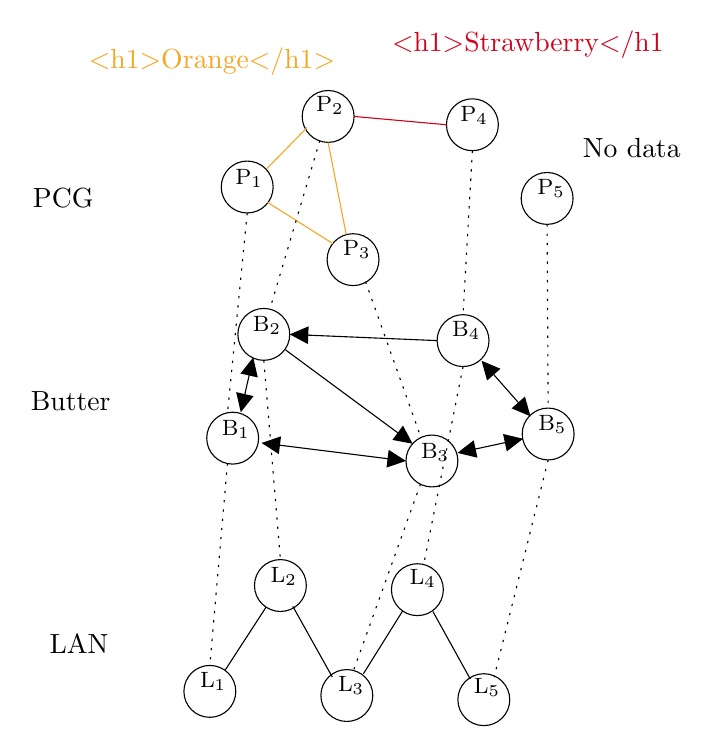
\begin{tikzpicture}[x=0.75pt,y=0.75pt,yscale=-1,xscale=1]
%uncomment if require: \path (0,451); %set diagram left start at 0, and has height of 451

%Shape: Circle [id:dp6061502443078786] 
\draw   (111,287.5) .. controls (111,280.6) and (116.6,275) .. (123.5,275) .. controls (130.4,275) and (136,280.6) .. (136,287.5) .. controls (136,294.4) and (130.4,300) .. (123.5,300) .. controls (116.6,300) and (111,294.4) .. (111,287.5) -- cycle ;
%Shape: Circle [id:dp36264343921365794] 
\draw   (126,237.5) .. controls (126,230.6) and (131.6,225) .. (138.5,225) .. controls (145.4,225) and (151,230.6) .. (151,237.5) .. controls (151,244.4) and (145.4,250) .. (138.5,250) .. controls (131.6,250) and (126,244.4) .. (126,237.5) -- cycle ;
%Shape: Circle [id:dp9971317502608965] 
\draw   (222,240.5) .. controls (222,233.6) and (227.6,228) .. (234.5,228) .. controls (241.4,228) and (247,233.6) .. (247,240.5) .. controls (247,247.4) and (241.4,253) .. (234.5,253) .. controls (227.6,253) and (222,247.4) .. (222,240.5) -- cycle ;
%Shape: Circle [id:dp9106166132377405] 
\draw   (263,285.5) .. controls (263,278.6) and (268.6,273) .. (275.5,273) .. controls (282.4,273) and (288,278.6) .. (288,285.5) .. controls (288,292.4) and (282.4,298) .. (275.5,298) .. controls (268.6,298) and (263,292.4) .. (263,285.5) -- cycle ;
%Shape: Circle [id:dp5541002056383258] 
\draw   (207,298.5) .. controls (207,291.6) and (212.6,286) .. (219.5,286) .. controls (226.4,286) and (232,291.6) .. (232,298.5) .. controls (232,305.4) and (226.4,311) .. (219.5,311) .. controls (212.6,311) and (207,305.4) .. (207,298.5) -- cycle ;
%Straight Lines [id:da3029168780037723] 
\draw    (154,237.63) -- (222,240.5) ;
\draw [shift={(151,237.5)}, rotate = 2.42] [fill={rgb, 255:red, 0; green, 0; blue, 0 }  ][line width=0.08]  [draw opacity=0] (8.93,-4.29) -- (0,0) -- (8.93,4.29) -- cycle    ;
%Straight Lines [id:da46957863774592223] 
\draw    (207.79,288.42) -- (149,245) ;
\draw [shift={(210.2,290.2)}, rotate = 216.45] [fill={rgb, 255:red, 0; green, 0; blue, 0 }  ][line width=0.08]  [draw opacity=0] (8.93,-4.29) -- (0,0) -- (8.93,4.29) -- cycle    ;
%Straight Lines [id:da9097415304582196] 
\draw    (245.38,252.45) -- (265.02,274.75) ;
\draw [shift={(267,277)}, rotate = 228.63] [fill={rgb, 255:red, 0; green, 0; blue, 0 }  ][line width=0.08]  [draw opacity=0] (8.93,-4.29) -- (0,0) -- (8.93,4.29) -- cycle    ;
\draw [shift={(243.4,250.2)}, rotate = 48.63] [fill={rgb, 255:red, 0; green, 0; blue, 0 }  ][line width=0.08]  [draw opacity=0] (8.93,-4.29) -- (0,0) -- (8.93,4.29) -- cycle    ;
%Straight Lines [id:da2061802483174313] 
\draw    (140.38,290.17) -- (204.02,298.13) ;
\draw [shift={(207,298.5)}, rotate = 187.13] [fill={rgb, 255:red, 0; green, 0; blue, 0 }  ][line width=0.08]  [draw opacity=0] (8.93,-4.29) -- (0,0) -- (8.93,4.29) -- cycle    ;
\draw [shift={(137.4,289.8)}, rotate = 7.13] [fill={rgb, 255:red, 0; green, 0; blue, 0 }  ][line width=0.08]  [draw opacity=0] (8.93,-4.29) -- (0,0) -- (8.93,4.29) -- cycle    ;
%Straight Lines [id:da9316247214989568] 
\draw    (234.73,293.97) -- (260.47,288.43) ;
\draw [shift={(263.4,287.8)}, rotate = 167.86] [fill={rgb, 255:red, 0; green, 0; blue, 0 }  ][line width=0.08]  [draw opacity=0] (8.93,-4.29) -- (0,0) -- (8.93,4.29) -- cycle    ;
\draw [shift={(231.8,294.6)}, rotate = 347.86] [fill={rgb, 255:red, 0; green, 0; blue, 0 }  ][line width=0.08]  [draw opacity=0] (8.93,-4.29) -- (0,0) -- (8.93,4.29) -- cycle    ;
%Straight Lines [id:da31757544534246873] 
\draw    (132.74,251.53) -- (128.06,272.07) ;
\draw [shift={(127.4,275)}, rotate = 282.8] [fill={rgb, 255:red, 0; green, 0; blue, 0 }  ][line width=0.08]  [draw opacity=0] (8.93,-4.29) -- (0,0) -- (8.93,4.29) -- cycle    ;
\draw [shift={(133.4,248.6)}, rotate = 102.8] [fill={rgb, 255:red, 0; green, 0; blue, 0 }  ][line width=0.08]  [draw opacity=0] (8.93,-4.29) -- (0,0) -- (8.93,4.29) -- cycle    ;
%Shape: Circle [id:dp39230600009532957] 
\draw   (100,409.5) .. controls (100,402.6) and (105.6,397) .. (112.5,397) .. controls (119.4,397) and (125,402.6) .. (125,409.5) .. controls (125,416.4) and (119.4,422) .. (112.5,422) .. controls (105.6,422) and (100,416.4) .. (100,409.5) -- cycle ;
%Shape: Circle [id:dp6725211407093591] 
\draw   (134,358.5) .. controls (134,351.6) and (139.6,346) .. (146.5,346) .. controls (153.4,346) and (159,351.6) .. (159,358.5) .. controls (159,365.4) and (153.4,371) .. (146.5,371) .. controls (139.6,371) and (134,365.4) .. (134,358.5) -- cycle ;
%Shape: Circle [id:dp534352110903068] 
\draw   (200,360.5) .. controls (200,353.6) and (205.6,348) .. (212.5,348) .. controls (219.4,348) and (225,353.6) .. (225,360.5) .. controls (225,367.4) and (219.4,373) .. (212.5,373) .. controls (205.6,373) and (200,367.4) .. (200,360.5) -- cycle ;
%Shape: Circle [id:dp5705459677432333] 
\draw   (232,413.5) .. controls (232,406.6) and (237.6,401) .. (244.5,401) .. controls (251.4,401) and (257,406.6) .. (257,413.5) .. controls (257,420.4) and (251.4,426) .. (244.5,426) .. controls (237.6,426) and (232,420.4) .. (232,413.5) -- cycle ;
%Shape: Circle [id:dp4884732451202879] 
\draw   (166,411.5) .. controls (166,404.6) and (171.6,399) .. (178.5,399) .. controls (185.4,399) and (191,404.6) .. (191,411.5) .. controls (191,418.4) and (185.4,424) .. (178.5,424) .. controls (171.6,424) and (166,418.4) .. (166,411.5) -- cycle ;
%Straight Lines [id:da5435068621925384] 
\draw    (139.5,369.07) -- (120,399.07) ;
%Straight Lines [id:da40058310101255523] 
\draw    (152.5,368.57) -- (171.5,402.57) ;
%Straight Lines [id:da745960373491508] 
\draw    (205.5,370.57) -- (186.5,401) ;
%Straight Lines [id:da9636103089067328] 
\draw    (220,371.07) -- (238,403.57) ;
%Straight Lines [id:da026025176740933853] 
\draw  [dash pattern={on 0.84pt off 2.51pt}]  (121,299.57) -- (112.5,397) ;
%Straight Lines [id:da8574677477453254] 
\draw  [dash pattern={on 0.84pt off 2.51pt}]  (138.5,250) -- (146.5,346) ;
%Straight Lines [id:da45830762125909896] 
\draw  [dash pattern={on 0.84pt off 2.51pt}]  (234.5,253) -- (215.5,348.57) ;
%Straight Lines [id:da692101028265002] 
\draw  [dash pattern={on 0.84pt off 2.51pt}]  (214,309.57) -- (181.5,400.07) ;
%Straight Lines [id:da20439957038676881] 
\draw  [dash pattern={on 0.84pt off 2.51pt}]  (275.5,298) -- (249.5,402.57) ;
%Shape: Circle [id:dp24822651082567027] 
\draw  [color={rgb, 255:red, 0; green, 0; blue, 0 }  ,draw opacity=1 ] (118,166.5) .. controls (118,159.6) and (123.6,154) .. (130.5,154) .. controls (137.4,154) and (143,159.6) .. (143,166.5) .. controls (143,173.4) and (137.4,179) .. (130.5,179) .. controls (123.6,179) and (118,173.4) .. (118,166.5) -- cycle ;
%Shape: Circle [id:dp425639162940066] 
\draw  [color={rgb, 255:red, 0; green, 0; blue, 0 }  ,draw opacity=1 ] (157,132.5) .. controls (157,125.6) and (162.6,120) .. (169.5,120) .. controls (176.4,120) and (182,125.6) .. (182,132.5) .. controls (182,139.4) and (176.4,145) .. (169.5,145) .. controls (162.6,145) and (157,139.4) .. (157,132.5) -- cycle ;
%Shape: Circle [id:dp15558332675817688] 
\draw  [color={rgb, 255:red, 0; green, 0; blue, 0 }  ,draw opacity=1 ] (169,201.5) .. controls (169,194.6) and (174.6,189) .. (181.5,189) .. controls (188.4,189) and (194,194.6) .. (194,201.5) .. controls (194,208.4) and (188.4,214) .. (181.5,214) .. controls (174.6,214) and (169,208.4) .. (169,201.5) -- cycle ;
%Shape: Circle [id:dp30081719961232734] 
\draw   (226.5,136.5) .. controls (226.5,129.6) and (232.1,124) .. (239,124) .. controls (245.9,124) and (251.5,129.6) .. (251.5,136.5) .. controls (251.5,143.4) and (245.9,149) .. (239,149) .. controls (232.1,149) and (226.5,143.4) .. (226.5,136.5) -- cycle ;
%Straight Lines [id:da8972847915279969] 
\draw [color={rgb, 255:red, 245; green, 166; blue, 35 }  ,draw opacity=1 ]   (139.8,157.8) -- (159.4,137.8) ;
%Straight Lines [id:da4060630063522047] 
\draw [color={rgb, 255:red, 245; green, 166; blue, 35 }  ,draw opacity=1 ]   (178.2,189.4) -- (169.5,145) ;
%Straight Lines [id:da6848460896070612] 
\draw [color={rgb, 255:red, 245; green, 166; blue, 35 }  ,draw opacity=1 ]   (140.2,173.8) -- (171.8,193.8) ;
%Straight Lines [id:da5819580495505107] 
\draw [color={rgb, 255:red, 208; green, 2; blue, 27 }  ,draw opacity=1 ]   (182,132.5) -- (226.5,136.5) ;
%Straight Lines [id:da49699117013802474] 
\draw  [dash pattern={on 0.84pt off 2.51pt}]  (130.5,179) -- (121,275.57) ;
%Straight Lines [id:da5794423519351266] 
\draw  [dash pattern={on 0.84pt off 2.51pt}]  (165.5,144.07) -- (141.5,225.07) ;
%Straight Lines [id:da9796158041739726] 
\draw  [dash pattern={on 0.84pt off 2.51pt}]  (187.5,212.07) -- (214,286.57) ;
%Straight Lines [id:da23772443967474888] 
\draw  [dash pattern={on 0.84pt off 2.51pt}]  (239,149) -- (234.5,228) ;
%Shape: Circle [id:dp47924057339080184] 
\draw   (262.5,172) .. controls (262.5,165.1) and (268.1,159.5) .. (275,159.5) .. controls (281.9,159.5) and (287.5,165.1) .. (287.5,172) .. controls (287.5,178.9) and (281.9,184.5) .. (275,184.5) .. controls (268.1,184.5) and (262.5,178.9) .. (262.5,172) -- cycle ;
%Straight Lines [id:da813689736444334] 
\draw  [dash pattern={on 0.84pt off 2.51pt}]  (275,184.5) -- (275.5,273) ;

% Text Node
\draw (26,166) node [anchor=north west][inner sep=0.75pt]   [align=left] {PCG};
% Text Node
\draw (34,381) node [anchor=north west][inner sep=0.75pt]   [align=left] {LAN};
% Text Node
\draw (25,264) node [anchor=north west][inner sep=0.75pt]   [align=left] {Butter};
% Text Node
\draw (53,98) node [anchor=north west][inner sep=0.75pt]   [align=left] {\textcolor[rgb]{0.96,0.65,0.14}{\lstinline|<h1>Orange</h1>|}};
% Text Node
\draw (199,90) node [anchor=north west][inner sep=0.75pt]   [align=left] {\textcolor[rgb]{0.82,0.01,0.11}{\lstinline|<h1>Strawberry</h1|}};
% Text Node
\draw (123.5,156.57) node [anchor=north west][inner sep=0.75pt]   [align=left] {{\footnotesize P\textsubscript{1}}};
% Text Node
\draw (162.5,121.57) node [anchor=north west][inner sep=0.75pt]   [align=left] {{\footnotesize P\textsubscript{2}}};
% Text Node
\draw (232,126.57) node [anchor=north west][inner sep=0.75pt]   [align=left] {{\footnotesize P\textsubscript{4}}};
% Text Node
\draw (269,161.57) node [anchor=north west][inner sep=0.75pt]   [align=left] {{\footnotesize P\textsubscript{5}}};
% Text Node
\draw (175.5,191.07) node [anchor=north west][inner sep=0.75pt]   [align=left] {{\footnotesize P\textsubscript{3}}};
% Text Node
\draw (117,277.57) node [anchor=north west][inner sep=0.75pt]   [align=left] {{\footnotesize B\textsubscript{1}}};
% Text Node
\draw (132,227.57) node [anchor=north west][inner sep=0.75pt]   [align=left] {{\footnotesize B\textsubscript{2}}};
% Text Node
\draw (213,288.57) node [anchor=north west][inner sep=0.75pt]   [align=left] {{\footnotesize B\textsubscript{3}}};
% Text Node
\draw (228,230.07) node [anchor=north west][inner sep=0.75pt]   [align=left] {{\footnotesize B\textsubscript{4}}};
% Text Node
\draw (269.5,275.07) node [anchor=north west][inner sep=0.75pt]   [align=left] {{\footnotesize B\textsubscript{5}}};
% Text Node
\draw (291,141.57) node [anchor=north west][inner sep=0.75pt]   [align=left] {No data};
% Text Node
\draw (106.5,399.07) node [anchor=north west][inner sep=0.75pt]   [align=left] {{\footnotesize L\textsubscript{1}}};
% Text Node
\draw (140.5,348.57) node [anchor=north west][inner sep=0.75pt]   [align=left] {{\footnotesize L\textsubscript{2}}};
% Text Node
\draw (173,401.07) node [anchor=north west][inner sep=0.75pt]   [align=left] {{\footnotesize L\textsubscript{3}}};
% Text Node
\draw (207.5,349.5) node [anchor=north west][inner sep=0.75pt]   [align=left] {{\footnotesize L\textsubscript{4}}};
% Text Node
\draw (238.5,402.07) node [anchor=north west][inner sep=0.75pt]   [align=left] {{\footnotesize L\textsubscript{5}}};


\end{tikzpicture}

    \caption{Example overlay structure with PCG}
    \label{fig:overlayPCG}
\end{figure}

% This is a illustrated example
Figure~\ref{fig:overlayPCG} illustrates an instance of a Butter network with a PCG overlay. In this example we see an underlying LAN network where the edges represent physical or local WIFI connections. The directed edges at the Butter level represent a node's known hosts and the edges in PCG layer represent group members.

The group of $P_1$, $P_2$ and $P_3$ are responsible for maintaining the information for the ``Orange" webpage. In the case that $r=3$ they are a complete group. The group $P_2$ and $P_4$ is responsible for ``Strawberry" but is in a cold state. In a cold state, a leader is elected amongst the two nodes and his responsibility is to find a node in his known hosts that is able to participate in the group. In this case, say that $P_4$ is elected leader, he interacts with the underlying butter node $B_4$ and sees that he has available known hosts $B_2$ and $B_5$. Say $B_5$ is asked to join the group, if it has the available storage, it will join and complete the group.

%\subsubsection{Request handler}
%
%A key feature of the original PCG implementation is that it allows for transparent content delivery despite high churn\cite{shinebourne2022availability}. All group members are responsible for responding to a request for information, and hence the burden does not fall on a specific node. This allows a request to be fulfilled despite the failure of the initial node responding to the request as if the initial peer fails, another peer will fulfil it. This has benefits for ease of implementation on the client side as there is no need to handle re-attempting to query the network for information if a request is unfinished, but has major drawbacks with network utilisation and implementation complexity. Therefore, Butter does not include this transparent interface and puts the responsibility of fulfilling a request on the client asking for the information. In other words, it is the client's responsibility to work to retrieve data, not that of the network.

\subsubsection{Extra optimisation}

% Geographic distribution
A $geo$ tag can be appended to each node's known host quality metric so when a leader is elected to find a new peer to join the group (if the group is deemed to be in an unsafe state) it will favour picking nodes with different $geo$ tags. This attempts to maximise the probability of redundant copies of information being distributed geographically, resulting in less shared infrastructure and improved information retrieval by reducing the average latency and steps taken to discover data.

\subsection{Testing \& evaluation}

In this section we will discuss how the design was tested as well as the different relationships between parameters such as heartbeat intervals and replication count. Based on the tests we evaluate the design and discuss some of the benefits and shortfalls of the implementation as well as what could be improved in future iterations.

\subsubsection{Methodology}
\label{sec:churnTesting}

The testing process is carries out as follows:

\begin{enumerate}
    \item The testbed generates $n$ nodes on different ports, each tasked with storing a random string of data.
    \item Test waits for nodes to spawn and form a network
    \item $chanceToDie$ and $churnTime$ parameters are specified. The $chanceToDie$ determines the probability that a node is terminated during the $churnTime$.
    \item Testbed churns the network and so simulates nodes failing over time. During churn new nodes are created to maintain the network node count at $n$.
    \item The network is left a moment to recover, allowing the remaining nodes to re-create and update their list of known hosts. New nodes are created to replace failed nodes, in order to maintain the number of nodes on the network.
    \item After a given period of time has passed, a new querying node is created with a list of all of the identifiers for information initially added to the network. The querying node attempts to retrieve all of the data that was initially stored in the network during initialisation. This node takes count of the number of successful and failed information queries, and so can provide a metric of the proportion of data that persisted on the network `post-churn'. The information retrieval algorithm used by the querying node is BFS (more on this in Section~\ref{sec:ir}). BFS allows for thorough exploration of the network so that we can be certain that the information is no present.
\end{enumerate}

% In addition, there is a centralised logging node used in development logging mode where peers frequently publish their stats to a centralised server which updates a database of nodes, their edges, properties and information they contaain - this allows for a visualisation of the current state of the network. It is important to note that this centralised server does not carry out any functionality and is simply used for logging the network. If nodes are unable to publish to the server they simply try again - publishing to the server cannot cause failure meaning that sometimes the loging can be incorrect.

\subsubsection{Results \& evaluation}

\begin{table}[ht]
    \centering
    \begin{tabular}{|l|l|l|}
        \hline
        Heartbeat interval (s) & Nb. messages sent & (\%) Success rate \\
        \hline
        10                     & 600               & 58.00             \\
        5                      & 1200              & 60.00             \\
        2                      & 3000              & 72.00             \\
        1                      & 6000              & 74.00             \\
        \hline
    \end{tabular}
    \caption{Experimental data from test rig. Tested on 100 simulated nodes, repeated 5 times at each heartbeat interval setting. \textbf{Note}: Messages sent is the cumulative amount of heartbeat messages sent between group participants over a 60s churn time, $chanceToDie$ was set to 1 in 50 across all heartbeat intervals.}
    \label{tab:heartbeatSuccess}
\end{table}

There were some initial issues with testing due to the speed of churn in simulation relative to the speed at which the nodes were carrying out heartbeats, i.e.\ the simulated churn rate was extremely high and heartbeat intervals too far apart. This was resolved by changing the heartbeat interval from 10s to 2s. This does increase the message complexity of the network greatly and so in practice the parameter should be considered carefully, based on the specifics of the network.

To demonstrate how message complexity scales with different heartbeat intervals and how heartbeat intervals influence information retention we can observe the data in Table~\ref{tab:heartbeatSuccess}. For a short interval $t_h$ (e.g.\ 1 or 2 seconds), the probability of all peers maintaining some data $X$ failing in between $t_h+t_r$ where $t_r$ is the time to recover to $n=r$, is very low. However, this requires the node to constantly flood the group with heartbeat queries and hence scales poorly.

%In the testing environment, we found 2 second heartbeat intervals to be a good compromise between maintaining groups effectively while reducing the heartbeat messages sent by a factor of 2 from a 1s heartbeat interval. This is an appropriate setting in the testing environment, however, in reality a greater heartbeat interval may be preferred as the churn rate may be less high in other practical instances of Butter networks.

When the initial tests were carried out\cite{shinebourne2022availability}, success rate was lower than expected. This turned out to be because heartbeat intervals were all in sync and hence inspired the design for heartbeat palpitations. Once palpitations were introduced and hence the intervals offset, success rate improved greatly.

\begin{table}[ht]
    \centering
    \begin{tabular}{|l|l|l|}
        \hline
        $chanceToDie$ & Nb. failed to retrieve & (\%) Success rate \\
        \hline
        1 in 50       & 63                     & 74.80             \\
        1 in 100      & 29                     & 88.40             \\
        1 in 1000     & 4                      & 98.40             \\
        1 in 10,000   & 0                      & 100.00            \\
        \hline
    \end{tabular}
    \caption{Experimental data collected from testbed. Tested on 250 simulated nodes, repeated 5 times at each $chanceToDie$; average is rounded to the closest node. \textbf{Note}: the $chanceToDie$ is per second, the network churn time was 30s and the heartbeats were set to every 2s.}
    \label{tab:chanceToDieResults}
\end{table}

In an effort to help interpret the data in Table~\ref{tab:chanceToDieResults}, think about the probability of an initially spawned node surviving churn when the $chanceToDie$ is 1 in 50. In that case, every second, for 30 seconds, each of the 250 nodes has a 1 in 50 chance of dying. In other words, for every second there is a $49/50$ chance of survival to the next second. The probability, therefore, of an initially spawned node surviving the churn stage of the testing process is $(\frac{49}{50})^{30}=0.545$. So, with a 1 in 50 $chanceToDie$, we can expect just above half the network to have failed over the course of the churn. With the persistent storage mechanism we have managed to retain on average 74.80\% of the original information. While this is not a perfect solution, it shows a significant improvement in terms of availability. The tests stressed the importance of choosing an appropriate heartbeat interval.

%\begin{table}[ht]
%    \centering
%    \begin{tabular}{|l|l|l|}
%        \hline
%        Group size & Nb. messages sent & (\%) Success rate \\
%        \hline
%        3          & 3000                & 74.80             \\
%        5          & 29                & 88.40             \\
%        10         & 4                 & 98.40             \\
%        \hline
%    \end{tabular}
%    \caption{Experimental data collected from test rig. Tested on 100 simulated nodes. \textbf{Note}: Chance to die was set to 1 in 100 and the heartbeat interval was set to 2s.}
%    \label{tab:group_size_results}
%\end{table}
%
%
%Finally, a last set of tests were carried out to provide insights into optimal group size. The group size can be user specified, and should be set cautiously, much like the heartbeat interval. Groups need to be sufficiently large so as to increase the probability of data retention but also small enough to make group maintenance efficient. As Table~\ref{tab:group_size_results} shows, group size will has a substantial effect on the amount of messages sent. Heartbeat may work for small group sizes but will not be suitable for larger groups.

Having carried out testing we can consider that the implemented solution has succeeded in providing a certain level of data persistence across a decentralised peer-to-peer network. Despite the limitations of the testbed, Table~\ref{tab:chanceToDieResults} shows that a significant amount of information that would otherwise have been lost, if no mechanisms for data persistence existed, was still present in the network after a period of relatively high simulated network churn.

An interesting future development might be to introduce dynamic group sizes\cite{ramaswamy2005clustering}. The groups and hence redundant copies of the data could dynamically grow with the popularity, i.e.\ frequency of access of a piece of information. This may improve availability for popular information, but more importantly, it would spread the load of information requests ensuring that average file download latency does not increase significantly for highly desired information. In addition it could increase the probability of $QUERYHIT$s in information retrieval. This will be further discussed in Section~\ref{sec:ir}.

Finally, PCG provides an elegant way of reasoning about persistent information on the network. The extension of PCG developed here improves the fault-tolerance and scalability of the original design by taking away some of the aspects that introduce centralisation, i.e.\ the publishing rendezvous super-peers. However, there is still a significant drawback in message complexity that will need to be addressed for networks at scale. A better future implementation may involve implementing randomised gossiping to solve the GMP, however, more testing will be needed.




    \newpage


\section{Information retrieval}
\label{sec:ir}

% \subsection{Problem statement}

Information Retrieval (IR) across an unstructured network is a graph search problem\cite{lv2002search}. Distributed search algorithms are designed to successfully locate resources while incurring low overhead (in time, space and message complexity)\cite{bisnik2005walk}.

In structured networks, the network topology can be exploited to increase search efficiency, this is not possible in an unstructured topology\cite{khatibi2021rd, li2005searching}. Hence, efficiently retrieving information is non-trivial in an unstructured network.

%A common `naive' approach in unstructured peer-to-peer information retrieval is to use Breadth-first search (BFS). While this has the benefit of simplicity, it floods the network with queries\cite{thampi2010replication}. Methods can be used to improve the performance of `naive' BFS such as including a time-to-live (ttl) for each query and implementing heuristics and metadata (see intelligent/directed BFS)\cite{tsoumakos2003p2pIr}. There are also significantly more efficient probabilistic approaches, e.g.\ random BFS, but those do not guarantee a full search through the network.

In short, the question can be posed as: how to find information quickly and efficiently while relying on a partial view of the network (the limited information available to a node) and not on a central repository of global knowledge. Solutions to this problem can be divided into two primary categories\cite{thampi2010replication}: blind, and informed.

% Not sure about this but could be good
% Inspired by Lamport's statement ``the popularity of the dining philosophers problem taught me that the best way to attract attention to a problem is to present it in terms of a story" we shall use the analogy of finding a book in a library to discuss information retrieval. Libraries are efficient for finding and retrieving a book as they are typically organised by a person, a librarian, with a global view of the system - without a consistent approach to organisation a library cannot be structured and the efficient mechanisms to search for a book within the library fail.
% even enforcing an alphabetical scheme to help make retrieval faster would require centralisation as we would need a node to allocate letters of the alphabet to each node entering the network

%One should make the distinction between locating and retrieving a known resource (i.e., searching by unique identifier) and searching for an unknown resource that may contain the desired information (i.e., a search engine). These are two distinct problems, in this case we are devising a solution for retrieving a specified piece of information and not designing a decentralised search engine.

% The IR module is intrinsically ties to the Persistent storage module as for IR to be necessary, the network needs to store information and the protocol for storing information dictates how information is identified. 

% Keys to improving the speed and efficiency of the information retrieval mechanism is to minimize the communication costs, that is, the number of messages sent between the peers, and to minimize the number of peers that are queried for each search request. 

\subsection{Related work}

In this section we present several techniques for information retrieval of a specified document on an unstructured peer-to-peer network. Typically flooding, random walks or expanding-rings are used to retrieve information stored by peers. Each peer visited will evaluate the query locally on its own content, and will support complex queries\cite{lua2005survey}.

\subsubsection{Gnutella `naive' breadth-first search}

BFS is the technique that was originally used in the Gnutella network and is illustrated in Figure~\ref{fig:gnutella}. The BFS search protocol in a peer-to-peer network is as follows: a querying node generates a $QUERY$ message which is propagated to all its known hosts. When a peer receives a $QUERY$ request, it searches its local storage for a match. If no match is found, it forwards the $QUERY$ to all of its known hosts (other than the sender). If some node $q$ receives the $QUERY$ and has a match in its local storage, $q$ generates a $QUERYHIT$ message to transmit the document. $QUERYHIT$ messages are sent along the same path that carried the $QUERY$ message\cite{zeinalipour2004ir}.

%When node $q$ receives a $QUERYHIT$ from more than one peer, it may decide to download the file from the peer with the best network connectivity.

\subsubsection{Extension to BFS with time-to-live}

The original Gnutella implementation of BFS sacrifices performance and network utilisation for the sake of simplicity. Each query consumes excessive network and processing resources because a query is propagated along all links (including nodes with high-latency)\cite{zeinalipour2004information}. This means a low bandwidth node can easily become a bottleneck. This became apparent as the Gnutella network became more popular and the search mechanisms failed to scale. One technique to avoid overusing network bandwidth is to associate each query with a time-to-live (TTL) parameter. The TTL parameter determines the maximum number of hops that a given query should be forwarded. In a typical value for the TTL is usually 7 and is decremented each time the query is forwarded. When the TTL becomes 0, the message is dropped. Note, some existing documents may not be located due to limited TTL\@.

\subsubsection{Random Breadth-first search technique}

Kalogeraki and Gunopulos propose an alternative to BFS, namely Random breadth-first search (RBFS) and evaluate its performance\cite{kalogeraki2002local}. They state that it can be a ``dramatic improvement over the `naive' BFS approach". In RBFS, a peer forwards a $QUERY$ to a random subset of its known hosts. The size of the subset can be a user specified parameter. The researchers suggest half of the peers ($0.5$) as in testing it proved the best compromise between IR success and message generation. RBFS, like the BFS mechanism, allows nodes to make local decisions quickly since they only needs to select a portion of their known hosts. However, this algorithm is probabilistic. It is possible that some large segments of the network may be unreachable because a node was unable to understand that a particular link would lead the query to a large segment of the network.\cite{zeinalipour2004information}

% \subsubsection{Random walker technique}

% The random walkers algorithm was originally proposed in 2002\cite{lv2002search}. The idea behind the approach is similar to that of RBFS. In Random walker, each node forwards a query message, called walker, randomly to one of its peers. To reduce the time to receive the results the idea of the walker is extended to a k-walker which after T steps is expected to reach approximately the same number of nodes as a 1-walker after kT steps. To prevent `walking' over the same nodes several times each node may retain states. The difference between RBFS and Rabdom walker is subtle, in RBFS each node forwards a query message to a fraction of its neighbors while in Random walker it is a specified conatnt of $k$. This results in the message complexity of RBFS remaining expentianl exponential, depsite being significantly more efficient than `naive' BFS, while in the k-Walker model the messages used is linear.

\subsubsection{Directed BFS with `Most Results in Past' heuristic}

In a directed BFS approach, each node forwards a query to a subset of its peers based on some heuristic. This technique was originally proposed by Yang et al. They compared a number of query routing heuristics and found that the `Most Results in Past' ($>RES$) heuristic was the most `satisfactory'\cite{yang2002efficient}. In other words, more documents were found in less steps using this heuristic. In $>RES$ a peer $q$ forwards a search message to $n$ peers which returned the most results for the last $k$ queries. In their experiments they chose $n=1$ and $k=10$ effectively turning Directed BFS into a directed Depth-first-search (DFS) approach. This technique may perform well because it routes queries to the larger network segments (which subsequently may also contain more relevant answers)\cite{zeinalipour2004information}.

\subsubsection{Intelligent Search Mechanism}

The Intelligent Search Mechanism (ISM) is a more sophisticated approach to Directed BFS with `Most Results in Past' heuristic\cite{kalogeraki2002local}. In an effort to minimise the number of queries made and improve search performance a peer estimates, for each query, which of its peers are more likely to reply to the query, and propagates the query message to those peers only. The mechanism consists of two components: a \textit{profiling mechanism} used by a node to build a profile of its known hosts (neighbouring peers) and a \textit{relevance rank} that uses the peer’s profiles to select the neighbours that will lead a query to the most relevant answers.
% The profiling mechanism is used to maintain the most recent queries, the corresponding queryhits along with the number of results.

\subsubsection{Gossiping to replicate global state}

A different approach to those previously discussed is, instead of searching based on a partial view of the network, to maintain a global state in a decentralised fashion using randomised gossipping. Cuenca-Acuna and Nguyen suggest an approach to constructing a content addressable publish/subscribe service that uses gossiping of global state across unstructured communities\cite{cuenca2002text}. Their framework is based on a global inverted index, i.e.\ a globally maintained map of content to its location. The inverted index is partially constructed by each node $n_k$, specifically, $n_k$ constructs a bloom filter $b_k$, of its local index and propagates it to the rest of the network using gossiping. A bloom filter is a space-efficient probabilistic data structure that is used to test whether an element is a member of a set, in this case it is an efficient way of representing if $n_k$ hosts the information. While this is an interesting approach, the paper does state that the technique does not scale and maintaining a global state across nodes may not be suitable for large network.\cite{zeinalipour2004ir}
% The global inverted index is then the collection of each node's bloom filters. Bloom filters are an attractive approach for distributed environments because they achieve smaller messages.

\subsection{Design \& implementation}

Gnutella showed us that a `naive' BFS is not a practical solution, as it floods the network with queries and so scales poorly for large networks. It is specially impractical as without a TTL there is no upper-bound to the breadth of search for a query. Each search query requires excessive network use and processing resources as a query is propagated along all links (including high latency links)\cite{zeinalipour2004ir}.

%Some particularly efficient solutions make use of structured elements such as super-peers, but, these approaches will not be considered as they re-introduce elements of centralisation.

%Blind search makes use of flooding techniques to relay queries to peers, where peers maintain no information about the P2P network or probable locations of objects(used in GNutella\cite{GNutella}). The informed search on the other hand maintains routing information based on popularity of objects, success rate, etc.  Despite better performance, due to the high overhead cost of informed search it is not being considered in this paper\cite{comparison_of_P2P_search}.

%It has been proven experimentally that random walk is better than randomised flooding for information retrieval\cite{walk_search}, in the condition of Peer clustering, where there are communities in the topology, with dense connectivity between Peers in the same group and sparse connectivity between Peers of different groups. ?need to say its relevant maybe? In the case of flooding, a user request is re-issued by the user(or the system on behalf of the user) multiple times in hopes of locating more resources, whereas the usage of `random walk' algorithm follows completely different trajectories and has a higher chance of locating new resources.

The design and implementation of the Butter Information retrieval (IR) module is largely inspired by the work carried out on later version of the Gnutella project (discussed in Chapter~\ref{ch:relatedProjects}). We did not implement a semi-centralised peer-to-peer architecture such as BitTorrent as by reintroducing centralised elements, in an effort to increase search efficiency, the resulting network is less fault-tolerant and hence less dependable. On the other hand, Butter's IR module needs to retrieve information efficiently in regard to time and message complexity to make application services built using the framework usable.

Butter implements a RBFS technique with a user specified TTL (per query). Having a user specified TTL allows the user to define how far they are willing to go to fetch a piece of information. Users also have the option to use a BFS mechanisms if the information is not found using the default RBFS mechanisms.

\begin{figure}[ht]
    \centering
    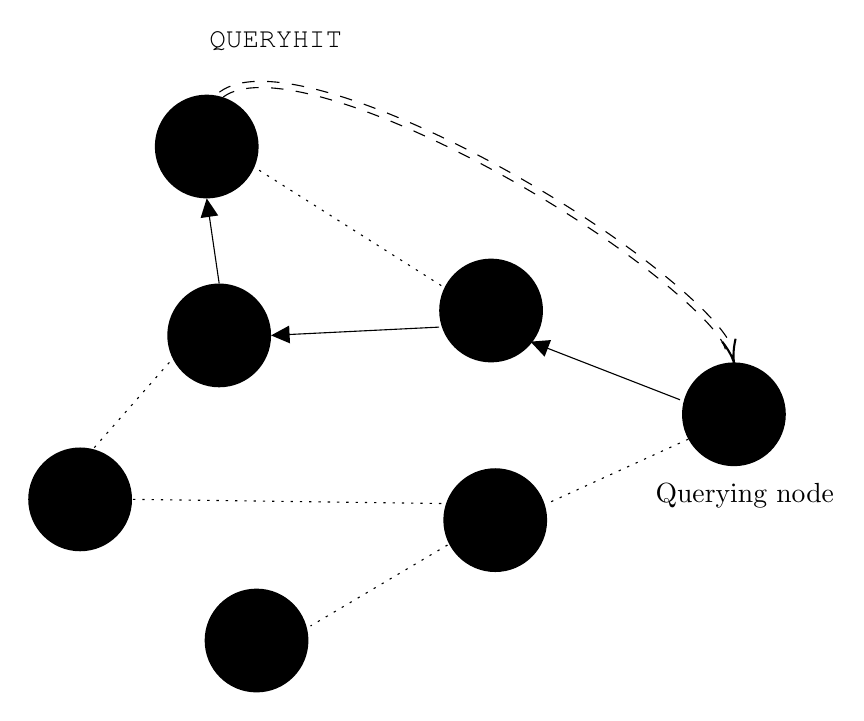
\begin{tikzpicture}[x=0.75pt,y=0.75pt,yscale=-1,xscale=1]
%uncomment if require: \path (0,451); %set diagram left start at 0, and has height of 451

%Shape: Circle [id:dp9331094894799612] 
    \draw  [draw opacity=0][fill={rgb, 255:red, 0; green, 0; blue, 0 }  ,fill opacity=1 ] (119,249) .. controls (119,235.19) and (130.19,224) .. (144,224) .. controls (157.81,224) and (169,235.19) .. (169,249) .. controls (169,262.81) and (157.81,274) .. (144,274) .. controls (130.19,274) and (119,262.81) .. (119,249) -- cycle ;
%Shape: Circle [id:dp9877389362602726]
    \draw  [draw opacity=0][fill={rgb, 255:red, 0; green, 0; blue, 0 }  ,fill opacity=1 ] (317,158) .. controls (317,144.19) and (328.19,133) .. (342,133) .. controls (355.81,133) and (367,144.19) .. (367,158) .. controls (367,171.81) and (355.81,183) .. (342,183) .. controls (328.19,183) and (317,171.81) .. (317,158) -- cycle ;
%Shape: Circle [id:dp0016664462798891]
    \draw  [draw opacity=0][fill={rgb, 255:red, 0; green, 0; blue, 0 }  ,fill opacity=1 ] (319,259) .. controls (319,245.19) and (330.19,234) .. (344,234) .. controls (357.81,234) and (369,245.19) .. (369,259) .. controls (369,272.81) and (357.81,284) .. (344,284) .. controls (330.19,284) and (319,272.81) .. (319,259) -- cycle ;
%Shape: Circle [id:dp3393753853906585]
    \draw  [draw opacity=0][fill={rgb, 255:red, 0; green, 0; blue, 0 }  ,fill opacity=1 ] (180,79) .. controls (180,65.19) and (191.19,54) .. (205,54) .. controls (218.81,54) and (230,65.19) .. (230,79) .. controls (230,92.81) and (218.81,104) .. (205,104) .. controls (191.19,104) and (180,92.81) .. (180,79) -- cycle ;
%Shape: Circle [id:dp6653810548572199]
    \draw  [draw opacity=0][fill={rgb, 255:red, 0; green, 0; blue, 0 }  ,fill opacity=1 ] (434,208) .. controls (434,194.19) and (445.19,183) .. (459,183) .. controls (472.81,183) and (484,194.19) .. (484,208) .. controls (484,221.81) and (472.81,233) .. (459,233) .. controls (445.19,233) and (434,221.81) .. (434,208) -- cycle ;
%Straight Lines [id:da22721998614149208]
    \draw    (433,201) -- (363.8,174.09) ;
    \draw [shift={(361,173)}, rotate = 21.25] [fill={rgb, 255:red, 0; green, 0; blue, 0 }  ][line width=0.08]  [draw opacity=0] (8.93,-4.29) -- (0,0) -- (8.93,4.29) -- cycle    ;
%Shape: Circle [id:dp23503433874211244]
    \draw  [draw opacity=0][fill={rgb, 255:red, 0; green, 0; blue, 0 }  ,fill opacity=1 ] (186,170) .. controls (186,156.19) and (197.19,145) .. (211,145) .. controls (224.81,145) and (236,156.19) .. (236,170) .. controls (236,183.81) and (224.81,195) .. (211,195) .. controls (197.19,195) and (186,183.81) .. (186,170) -- cycle ;
%Curve Lines [id:da8258695712571896]
    \draw  [dash pattern={on 4.5pt off 4.5pt}]  (211.1,52.8) .. controls (215.83,49.25) and (222.64,47.57) .. (231.07,47.57) .. controls (255.64,47.57) and (294.25,61.83) .. (332.86,81.67) .. controls (356.91,94.02) and (380.97,108.53) .. (401.61,123.04) .. controls (432.52,144.78) and (455.66,166.59) .. (457.83,175.9)(212.9,55.2) .. controls (217.2,51.97) and (223.44,50.57) .. (231.07,50.57) .. controls (255.32,50.57) and (293.4,64.77) .. (331.49,84.33) .. controls (355.42,96.63) and (379.35,111.06) .. (399.88,125.5) .. controls (430.01,146.68) and (452.89,167.79) .. (454.87,176.66) ;
    \draw [shift={(459,183)}, rotate = 257.2] [color={rgb, 255:red, 0; green, 0; blue, 0 }  ][line width=0.75]    (10.93,-3.29) .. controls (6.95,-1.4) and (3.31,-0.3) .. (0,0) .. controls (3.31,0.3) and (6.95,1.4) .. (10.93,3.29)   ;
%Straight Lines [id:da49607654384730693]
    \draw  [dash pattern={on 0.84pt off 2.51pt}]  (318,146) -- (228,89) ;
%Straight Lines [id:da7736178088954417]
    \draw    (317,166) -- (239,169.85) ;
    \draw [shift={(236,170)}, rotate = 357.17] [fill={rgb, 255:red, 0; green, 0; blue, 0 }  ][line width=0.08]  [draw opacity=0] (8.93,-4.29) -- (0,0) -- (8.93,4.29) -- cycle    ;
%Straight Lines [id:da4613250022232429]
    \draw  [dash pattern={on 0.84pt off 2.51pt}]  (187,183) -- (150,225) ;
%Straight Lines [id:da5738181000901116]
    \draw  [dash pattern={on 0.84pt off 2.51pt}]  (437,220) -- (369,251) ;
%Shape: Circle [id:dp11048151315696086]
    \draw  [draw opacity=0][fill={rgb, 255:red, 0; green, 0; blue, 0 }  ,fill opacity=1 ] (204,317) .. controls (204,303.19) and (215.19,292) .. (229,292) .. controls (242.81,292) and (254,303.19) .. (254,317) .. controls (254,330.81) and (242.81,342) .. (229,342) .. controls (215.19,342) and (204,330.81) .. (204,317) -- cycle ;
%Straight Lines [id:da9165977584013065]
    \draw    (211,145) -- (205.43,106.97) ;
    \draw [shift={(205,104)}, rotate = 81.67] [fill={rgb, 255:red, 0; green, 0; blue, 0 }  ][line width=0.08]  [draw opacity=0] (8.93,-4.29) -- (0,0) -- (8.93,4.29) -- cycle    ;
%Straight Lines [id:da5283181536620382]
    \draw  [dash pattern={on 0.84pt off 2.51pt}]  (318,251) -- (169,249) ;
%Straight Lines [id:da7410818285653099]
    \draw  [dash pattern={on 0.84pt off 2.51pt}]  (321,271) -- (255,310) ;

% Text Node
    \draw (205,22) node [anchor=north west][inner sep=0.75pt]   [align=left] {{\fontfamily{pcr}\selectfont QUERYHIT}};
% Text Node
    \draw (420,240) node [anchor=north west][inner sep=0.75pt]   [align=left] {Querying node};


\end{tikzpicture}

    \caption{Successful RBFS on Butter}
    \label{fig:succesfulRBFS}
\end{figure}

\noindent The RBFS implementation in Butter is as follows:
\begin{itemize}
    \item A peer $i$ generates a $QUERY$ message which is propagated to a random subset of its neighbors (known hosts)
    \item When a peer $j$ receives a $QUERY$ request, it first checks if it possesses the queried data in its local repository.
    \begin{itemize}
        \item If it does, it returns the information with a $QUERYHIT$ message.
        \item Else, it propagates the $QUERY$ to a random subset of its neighbours
    \end{itemize}
\end{itemize}

The proportion of the known hosts selected can be user specified. If unspecified it defaults to $0.5$. An example successful run is illustrated in Figure~\ref{fig:succesfulRBFS}.

Butter stores information in a `chunk' data structure. which contains a 4kb array for information, some optional keywords to associate with that information, and a $part/totalParts$ number. If the data is smaller that 4kb then it is stored in a single chunk, else, when data is added to the network, it is broken down into several `chunks' with the appropriate part number.

Information is uniquely identified by the hash of the whole information and a chunk number. Initially a query search is based on the hashed information regardless of the chunk number, simply finding the first hash match. Once an initial hit is made, the querying node learns about the number of chunks and hence generates queries for all the remaining parts. This enables the rest of the search to be carried out in parallel and improves retrieval speed.

\subsection{Testing \& Evaluation}

Using the tested, we spawned nodes and stored random information strings in each of the nodes. We stored the information identifiers in a global database and then spawned another node to systematically query each of the spawned nodes. We measured the average number of messages generated, documents found as well as the average time taken for the `naive' BFS and RBFS with TTL search mechanisms.

\begin{table}[ht]
    \centering
    \begin{tabular}{|l|l|l|l|}
        \hline
        Technique & Avg number of messages & (\%) Documents found  & Avg time taken (seconds) \\
        \hline
        BFS       & 587               & 100                   & 10.1 \\
        RBFS      & 235                & 68                    & 5.4 \\
        \hline
    \end{tabular}
    \caption{Comparing information retrieval techniques. Carried out for 10 queries on 100 simulated nodes.}
    \label{tab:irTechniques}
\end{table}

\begin{figure}[ht]
    \centering
    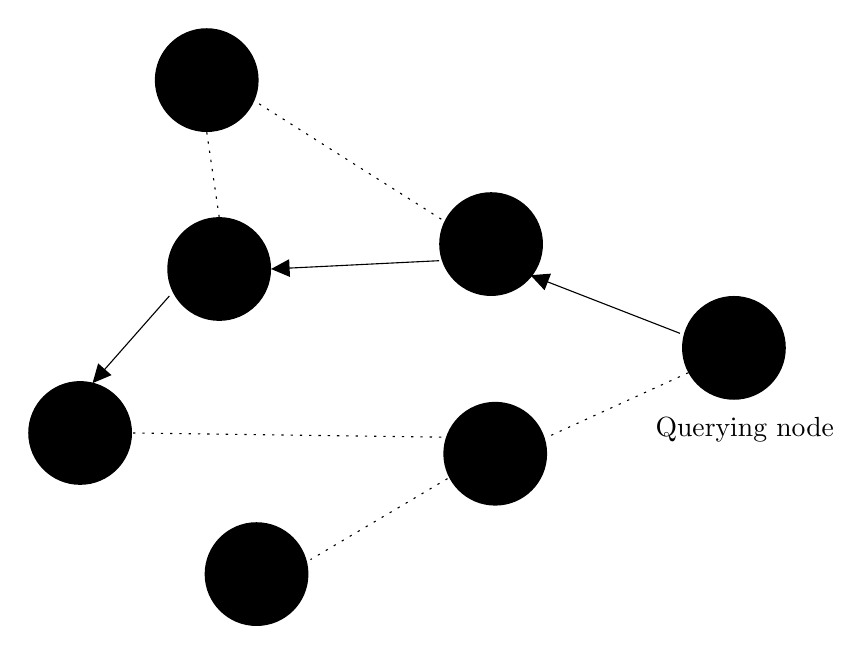
\begin{tikzpicture}[x=0.75pt,y=0.75pt,yscale=-1,xscale=1]
%uncomment if require: \path (0,451); %set diagram left start at 0, and has height of 451

%Shape: Circle [id:dp9331094894799612] 
    \draw  [draw opacity=0][fill={rgb, 255:red, 0; green, 0; blue, 0 }  ,fill opacity=1 ] (119,249) .. controls (119,235.19) and (130.19,224) .. (144,224) .. controls (157.81,224) and (169,235.19) .. (169,249) .. controls (169,262.81) and (157.81,274) .. (144,274) .. controls (130.19,274) and (119,262.81) .. (119,249) -- cycle ;
%Shape: Circle [id:dp9877389362602726] 
    \draw  [draw opacity=0][fill={rgb, 255:red, 0; green, 0; blue, 0 }  ,fill opacity=1 ] (317,158) .. controls (317,144.19) and (328.19,133) .. (342,133) .. controls (355.81,133) and (367,144.19) .. (367,158) .. controls (367,171.81) and (355.81,183) .. (342,183) .. controls (328.19,183) and (317,171.81) .. (317,158) -- cycle ;
%Shape: Circle [id:dp0016664462798891] 
    \draw  [draw opacity=0][fill={rgb, 255:red, 0; green, 0; blue, 0 }  ,fill opacity=1 ] (319,259) .. controls (319,245.19) and (330.19,234) .. (344,234) .. controls (357.81,234) and (369,245.19) .. (369,259) .. controls (369,272.81) and (357.81,284) .. (344,284) .. controls (330.19,284) and (319,272.81) .. (319,259) -- cycle ;
%Shape: Circle [id:dp3393753853906585] 
    \draw  [draw opacity=0][fill={rgb, 255:red, 0; green, 0; blue, 0 }  ,fill opacity=1 ] (180,79) .. controls (180,65.19) and (191.19,54) .. (205,54) .. controls (218.81,54) and (230,65.19) .. (230,79) .. controls (230,92.81) and (218.81,104) .. (205,104) .. controls (191.19,104) and (180,92.81) .. (180,79) -- cycle ;
%Shape: Circle [id:dp6653810548572199] 
    \draw  [draw opacity=0][fill={rgb, 255:red, 0; green, 0; blue, 0 }  ,fill opacity=1 ] (434,208) .. controls (434,194.19) and (445.19,183) .. (459,183) .. controls (472.81,183) and (484,194.19) .. (484,208) .. controls (484,221.81) and (472.81,233) .. (459,233) .. controls (445.19,233) and (434,221.81) .. (434,208) -- cycle ;
%Straight Lines [id:da22721998614149208] 
    \draw    (433,201) -- (363.8,174.09) ;
    \draw [shift={(361,173)}, rotate = 21.25] [fill={rgb, 255:red, 0; green, 0; blue, 0 }  ][line width=0.08]  [draw opacity=0] (8.93,-4.29) -- (0,0) -- (8.93,4.29) -- cycle    ;
%Shape: Circle [id:dp23503433874211244] 
    \draw  [draw opacity=0][fill={rgb, 255:red, 0; green, 0; blue, 0 }  ,fill opacity=1 ] (186,170) .. controls (186,156.19) and (197.19,145) .. (211,145) .. controls (224.81,145) and (236,156.19) .. (236,170) .. controls (236,183.81) and (224.81,195) .. (211,195) .. controls (197.19,195) and (186,183.81) .. (186,170) -- cycle ;
%Straight Lines [id:da49607654384730693] 
    \draw  [dash pattern={on 0.84pt off 2.51pt}]  (318,146) -- (228,89) ;
%Straight Lines [id:da7736178088954417] 
    \draw    (317,166) -- (239,169.85) ;
    \draw [shift={(236,170)}, rotate = 357.17] [fill={rgb, 255:red, 0; green, 0; blue, 0 }  ][line width=0.08]  [draw opacity=0] (8.93,-4.29) -- (0,0) -- (8.93,4.29) -- cycle    ;
%Straight Lines [id:da4613250022232429] 
    \draw    (187,183) -- (151.98,222.75) ;
    \draw [shift={(150,225)}, rotate = 311.38] [fill={rgb, 255:red, 0; green, 0; blue, 0 }  ][line width=0.08]  [draw opacity=0] (8.93,-4.29) -- (0,0) -- (8.93,4.29) -- cycle    ;
%Straight Lines [id:da5738181000901116] 
    \draw  [dash pattern={on 0.84pt off 2.51pt}]  (437,220) -- (369,251) ;
%Shape: Circle [id:dp11048151315696086] 
    \draw  [draw opacity=0][fill={rgb, 255:red, 0; green, 0; blue, 0 }  ,fill opacity=1 ] (204,317) .. controls (204,303.19) and (215.19,292) .. (229,292) .. controls (242.81,292) and (254,303.19) .. (254,317) .. controls (254,330.81) and (242.81,342) .. (229,342) .. controls (215.19,342) and (204,330.81) .. (204,317) -- cycle ;
%Straight Lines [id:da9165977584013065] 
    \draw  [dash pattern={on 0.84pt off 2.51pt}]  (211,145) -- (205,104) ;
%Straight Lines [id:da5283181536620382] 
    \draw  [dash pattern={on 0.84pt off 2.51pt}]  (318,251) -- (169,249) ;
%Straight Lines [id:da7410818285653099] 
    \draw  [dash pattern={on 0.84pt off 2.51pt}]  (321,271) -- (255,310) ;

% Text Node
    \draw (420,240) node [anchor=north west][inner sep=0.75pt]   [align=left] {Querying node};


\end{tikzpicture}

    \caption{Failed RBFS on Butter}
    \label{fig:failedRBFS}
\end{figure}

Table~\ref{tab:irTechniques} shows a clear improvement in message complexity using a RBFS approach over BFS. However, the \% of successfully retrieved documents is significantly lower. There is a compromise to be made between speed, message complexity and success rate. A failed scenario of RBFS is depicted in Figure~\ref{fig:failedRBFS}. The value of the proportion of known hosts selected at random could be tweaked from the default $0.5$ to other values to improve the success rate.

Two features mentioned in the Persistent storage section could have an impact on IR performance. We mention a node geotag enabling information to be spread geographically which in turn would improve resilience. This may also help minimise latency and hence improves search time. In addition, dynamic group sizes based on the perceived popularity of a piece information, i.e.\ information that is frequently queried, may increase the probability of a hit and spreads the load across more nodes, however, this would have to be further tested.

In their work Zeinalipour and Gunopulos\cite{zeinalipour2004information} have shown, we can greatly improve the \% successful document retrieval while maintaining similarly efficient message complexity to RBFS by using an informed approach. RBFS does not use any explicit technique to guide the search query to the most relevant content, which is a desirable property in information retrieval. A future implementation will look at implementing an informed approach; most probably the Intelligent Search Mechanism.


    \chapter{Case studies}
\label{sec:caseStudies}

% present a balanced argument for why a decentralised chat i.e. pros/cons decentralised communication protocols
% present a balanced argument for why a decentralised wiki i.e. pros/cons decentralised encyclopedic information protocols

% Intro
While so far we have explored the design and implementation of the framework, it is important to also explore how the framework will be used to develop decentralised applications. Three example decentralised applications were implemented alongside Butter to test features and the development experience. One of the simplest examples was a reverse echo application where a user submits a string to the service, and it returns a reverse of the string, the processing happening elsewhere on the network. While this is not an interesting application, it provided grounds for testing. Two significantly more compelling case studies were explored: a decentralised chat application and wiki application. The chat and wiki application demonstrate the advantages of decentralisation for communication and high availability information storage respectively.

% Decentralised communication case study - simple peer-to-peer chat
Decentralised chat applications are a fascinating service case study as decentralised communication goes back to the original roots of the Internet's inception. ARPNET the predecessor to the Internet, which laid the foundational groundwork for the technology, was conceived as a ``computer communications system without a central core, with no headquarters or base of operations that could not be attacked and destroyed by enemies thus blacking out the entire network in one fell swoop"\cite{featherly2022arpnet}. To contextualise, this research was carried out at the height of the cold war. In addition, it seems intuitive to design communication systems in a decentralised way. As humans, this is typically how we navigate and communicate in our daily lives. However, as systems grow in user-base, it becomes natural to employ structured mechanisms to manage communication complexity.

In recent decades we have seen the rise of cloud services, i.e.\ services provided by third-parties\cite{redhat2022cloud}. Since this shift, we have blindly moved our habits to these services, for practicality as they are presented as highly reliable and dependable. Many of these services become viable businesses by either asking for user subscriptions in exchange for use or more commonly monetising their service through advertisement revenue. The resulting services, are often propriety, centralised and out of the user's control. This poses an interesting question: should we allow ourselves to become highly dependent on cloud services, specially for communication services that are so fundamental to our daily lives. If we can trust the cloud service providers, the problem is mute, if not, this model of service delivery cannot be sustained\cite{benkler2016degrees}.

Butter's demo chat application allows direct peer-to-peer communication between peers on the same LAN. This application is still rudimentary and will be further extended to enable direct peer-to-peer communication across the internet once the Wider discovery module is further tested.

% Decentralised information storage - simple wiki
The other case study for a Butter application is a wiki. A wiki can be thought of as a, typically community information driven, encyclopedia service. It is a particularly pertinent case study for an application of a fault-tolerant decentralised information service. The information in a wiki tends to be provided by contributing members of the community. There is no single author and hence it can be difficult to attribute information to any single figurehead. This model of information service brings about some interesting questions: Who owns the information? Who is responsible for the information and the consequences of its dissemination? Who maintains and hosts the service? In certain scenarios, the service can be of immense value to its users and society more broadly, so, it is important that the service be dependable and highly available. In addition, ubiquitous access to information may be desirable for a service, so it needs to be designed to be devoid of central control and censorship.

Some wikis are hosted and maintained by purely altruistic organisations and individuals. However, this is not always the case, and in some cases it is wise to consider whether we should trust private third-parties to have the interests of the community at heart. This problem could be avoided if the service were delivered by an autonomous decentralised network where, like the information, the infrastructure would be community contributed as well.

In Butter's wiki demo, the application behaves similarly to a typical wiki. Users can publish and retrieve informative articles, but it is significant to note that there is no central server, the information is not stored in a central index or hosted by a single third-party. Each node instance running the service has never explicitly been made aware of others, yet the service is still delivered. Nodes work together to maintain the information using the PCG mechanisms and the Information retrieval module handles decentralised search across the network removing the need for a central database. This has the effect of creating an autonomous service.

Having said that, there are still severe limitations with Butter and decentralised service delivery more broadly. Something that has been made clear throughout the literature is that the problem of scalable decentralised services has yet to be solved. In addition, it is important to note that not all services should or need to be autonomously delivered. There is a case that services involving personal information should not be autonomous.

% Blog
Take the example of a blog or social media sharing platform. These platforms may deal with personal information which should be considered with caution. Butter is not yet equipped to deal with personal information. Currently, there are no inbuilt encryption mechanisms and while the autonomy means information is devoid of malicious control it makes controlling personal information on the network difficult. This is further discussed in the legal, social and ethical considerations section (see~\ref{legalSocialEthical}) of the project.

% Probabilities
% Something to note is that in a complex environment, a service will always have a probability associated with its successful delivery. Decentralised systems can seem fault prone because they openly disclose that there operations have a certain probability of functioning. Cloud services tend to present themselves as a certainty, but like all systems they also have a probability of failure. Hence successufly retrieving a piece of information on Butter or Google drive both have probabilities associated with them.



    \chapter{Conclusion}
\label{ch:conclusion}


\section{Summary}
\label{sec:summary}

This report has introduced some core concepts in distributed architectures and how they can give rise to decentralised systems. We have described two common types of peer-to-peer architectures: unstructured and structured, and discussed their benefits and limitations. Furthermore, we introduced the motivations and major contributions of this work. In Chapter~\ref{ch:relatedProjects} we gave an overview of several significant projects both past and present focused on building peer-to-peer systems. Aspects of the project's management were discussed in the ensuing chapter where we briefly justify the decision to gravitate towards an incremental development model and present some turning points in the project's development.

The technical detail for the project is contained within Chapter~\ref{ch:buildingButter}. There, each module of the framework was described and evaluated in detail. The core problems presented are: local peer discovery, NAT traversal and internet discovery, peer selection, persistent information storage and information retrieval. Each module of the framework attempts to provide a decentralised solution to one or more of these problems. The report finishes by discussing some case studies that present interesting arguments and open a debate about decentralised systems and the resulting autonomy of the services they provide.


\section{Butter vs. libp2p}

It may be interesting to briefly look at how Butter compares to its closest neighbour: \verb+libp2p+.

Having initially been sceptical of \verb+libp2p+, I have a much better appreciation for its design having built a peer-to-peer framework myself. The concept of multiadddresses is a particularly ingenious way of creating generalised nodes which are capable of providing infrastructure to deliver many types of services. In addition, \verb+libp2p+'s focus on modular design enables developers to use it for specific problems they encounter without needing to convert their entire existing system to the framework. \verb+libp2p+'s specification is implemented in JavaScript, Go and Rust with future plans for Python, Java and Haskell which should help make it a ubiquitous solution to designing peer-to-peer systems regardless of the language of choice\cite{protocollabs2022implementations}.

Furthermore, another particularly good feature of \verb+libp2p+, is that it is independent of any specific transport layer, making it more flexible and adaptable to different use cases. In addition, the project's focus on high quality documentation and promoting research into p2p system has been a valuable contribution the field.

% As Butter evolved elements started to feel more and more like \verb+libp2p+. The philosophy of modular design is definitely inspired by \verb+libp2p+. In future, it would be good to generalise Butter so that it is not restrict to a TCP transport protocol like libp2p.


\section{Future work}

While we have mentioned possible improvements to the individual Butter modules in their respective sections we have not yet discussed broader future directions for the project. It is my full intention to continue to research and improve the Butter framework.

Since the project's first open source publication, several developers have been in contact discussing possibilities to collaborate and exchange ideas. This is tremendously exciting and there is a lot of work to be done as the problem of scalable decentralised systems has yet to be solved. In addition, I have been in contact with the developers at Protocol labs (libp2p) and the Maidsafe project (SAFE network) discussing future roles and possibilities for contribution.

One of the first improvements to make would be to develop a significantly more robust testbed. One of the main limiting factors in progress and research for the project was testing, so improved testing utilities would be beneficial. It would be particularly interesting to expand on the work of Zeinalipour on PeerWare\cite{zeinalipour2005peerware}. PeerWare is a testbed for information retrieval on peer-to-peer networks that enables specific instances of network topologies. Adding this functionality to the Butter testbed would enable better exploration of edge cases particularly for the Known host management module.

Another interesting direction for the project would be to integrate a Butter node with a browser; similar to what is being done by the Beaker Browser project\cite{dat2022beaker}. This has been an initial long-term goal for the project as it provides an elegant means of inciting contribution to the network. This design would support a future Internet consumption model where users are expected to contribute resources as they consume services available on the Internet. The effect would be similar to that of the `tit-for-tat' BitTorrent protocol were once you download a file you are expected to host it for others (seeding).

Throughout the project, Adam Chester and I have discussed the possibility of collaborating on a paper. The intention would be to provide a summative review of the various problems and protocols present in unstructured peer-to-peer architectures. Furthermore, some more work needs to be carried out on the Peer selection problem which is not widely been researched thus far as most research is focused on structured approaches to generate network topologies. In addition, further extensions to the PCG mechanisms will be required before the network could be widely deployed (see section~\ref{legalSocialEthical}).


\section{Legal, social and ethical considerations}
\label{legalSocialEthical}

Peer-to-peer systems are both a technical and social phenomenon\cite{glorioso2010social}. As Gnutella has shown, they can be associated with a host of legal and ethical considerations. Notably, peer-to-peer systems have been notoriously used to share information protected by copyright law. This was both the case on the Gnutella network and on some BitTorrent networks.

Allusions have already been made in Section~\ref{sec:caseStudies} to the limitations of decentralised and autonomous networks in regard to information management. Focusing specifically on Butter, there is currently no option to update or remove information from the network. The PCG mechanism can, in its current form, only store information, and thus far has been entirely focused on information persistence.

The `right to be forgotten'\cite{globocnjik2020right} and the right to update and correct information cannot be met in the current implementation of Butter. It will be necessary, before Butter can be put into practical use, to extend PCG to enable $update$ and $delete$ operations as we have a legal and ethical responsibility to design systems that allow incorrect information to be modified and comply with the `right to be forgotten'.


\section{Author's assessment of the project}

This project has been fascinating, and I am pleased with my new-found knowledge and proud of the resulting work. I distinctly remember how it exciting it was when the peer discovery mechanisms first started working, being able to see two entirely independent computers become aware of each other's existence. I am particularly pleased with the work on the persistent information storage mechanisms and find the idea of autonomous networks enticing.

This project has allowed me to gain a significant level of expertise in the field of decentralised peer-to-peer systems, and it has without doubt become one of my passions. The framework is open source and is my first project to gain traction in the open-source community. I have had several individuals approach me with a desire for collaboration and have even received a job offer based on the work carried out for the project.

%Finally, it is a matter of personal satisfaction that a version of this report is now hosted on a Butter network.

% Culmination of a year work - I'm quite proud of it, and I have fallen in love with distributed and decentralised systems


    \bibliographystyle{ieeetr}
    \bibliography{citations}

    \appendix

    \chapter{Original objectives}
\label{objectives}

For the readers convenience, here bellow lies the objectives from original project specification.

\section{Functional objective}
\begin{enumerate}
    \item Design and implement a decentralised application platform.
          \begin{enumerate}
              \item Implement rudimentary TCP communication between peers
              \item Implement peer discovery mechanism
              \item Implement data structure commonly understood by the peer-to-peer network nodes (most likely a decentralised hashtable)
              \item Implement an addressing mechanism, possibly content-based addressing
              \item Implement mechanism in which network data consistency is managed with node exit
              \item Implement agent nodes that help maintain data consistency even with node failure % this was not implemented as PCG the functionality was provided by PCGs
          \end{enumerate}
    \item Build a knowledge base/encyclopedia Wikipedia style application on top as a case study.
          \begin{enumerate}
              \item Use decentralised platform API to store encyclopedia content
              \item Design a method of accessing and visualising the content
          \end{enumerate}
\end{enumerate}

\section{Non-functional objectives}
\begin{enumerate}
    \item Learn Rust/Go/JS
    \item Lean about decentralised networks
    \item Learn about historic and new approaches to the decentralisation problem
    \item Propose a use case where users contribute as peers whilst navigating the application on the decentralised platform
    \item Discuss the legal, ethical and social impacts of a decentralised knowledge base
    \item Contribute a valuable learning resource to newcomers (such as myself) getting started with decentralised systems
\end{enumerate}

\section{Possible extensions}
A possible extension would be to achieve a use case, where a user using a decentralised application, in exchange, contributes resources to the decentralised network similar to how 'torrenting' or the Beaker Browser work. As a user views and downloads files, they also host them for others on the network.

\section{Out of scope}
Enabling the network to connect to peers over the Internet, while being exciting, is out of scope for the project. The Internet adds a layer of complexity as peer discovery is problematic on a network as extensive as the Internet. Discovering peers would require Network Address Translation, moving from one sub-network to another, which is challenging to do in a decentralised way.
    \chapter{Original timeline}

Original timeline taken from the project specification.

\label{originalTimeline}

\begin{figure}[h]
    \centering
    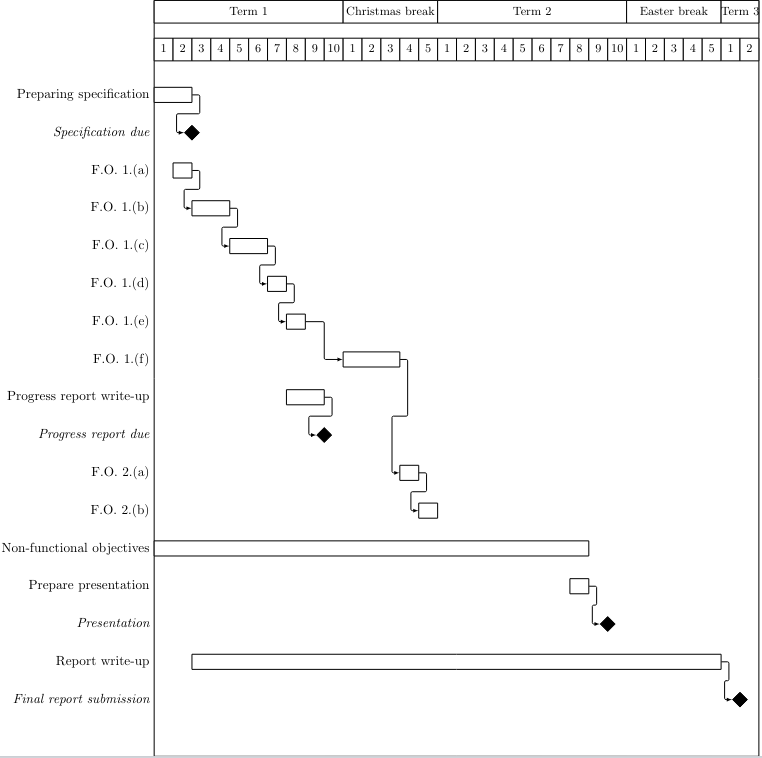
\includegraphics[width=\textwidth]{imgs/Screenshot from 2022-04-05 16-16-55.png}
\end{figure}
    \chapter{Revised timeline}
\label{actualTimeline}

Here bellow is an accurate timeline of the progress of the project. This timeline, taken from the project presentation slides, gives a loose overview of the key tasks carried out during the project's development.

\begin{itemize}
    \item \textbf{Summer 2021}
          \begin{itemize}
              \item Started learning about blockchains, IPFS, libp2p, Chord and Kademlia DHTs
          \end{itemize}

    \item \textbf{Term 1}
          \begin{itemize}
              \item Getting to grip with distributed (decentralised) systems
              \item Learning about Rust and systems/network programming
              \item Reading academic literature on Information Retrieval in unstructured architectures
              \item Completion of the Discovery and Wider discovery modules
              \item Implementation of naive protocols for Known host management, and Persistent storage modules (allowed for testing and experimentation)
          \end{itemize}

    \item \textbf{Christmas break}
          \begin{itemize}
              \item Implementation of IR using BFS in the Information retrieval module
              \item Switch from Rust to Go
              \item Starting to write up project documentation
          \end{itemize}

    \item \textbf{Term 2}
          \begin{itemize}
              \item Reading literature on persistence storage on high churn unstructured p2p systems
              \item Implementation of intelligent known host management optimising for diversity
              \item Implementation of persistent storage based on PCG overlay
          \end{itemize}
\end{itemize}
    \chapter{List of JXTA protocols}
\label{jxtaProtocols}

Project JXTA has defined six protocols so far.
\begin{itemize}
    \item Peer Discovery Protocol—enables a peer to find advertisements on
other peers and can be used to find any of the peer, peer group, or adver-
tisements.This protocol is the default discovery protocol for all peer groups,
including theWorld Peer Group. It is conceivable that someone might want
to develop a premium discovery mechanism that might or might not choose
to leverage this default protocol, but the inclusion of this default protocol
means that all JXTA peers can understand each other at the very basic level.
Peer discovery can be done with or without specifying a name for
either the peer to be located or the group to which peers belong.When
no name is specified, all advertisements are returned.
\item Peer Resolver Protocol—enables a peer to send and receive gener-
ic queries to search for peers, peer groups, pipes, and other informa-
tion.Typically, this protocol is implemented only by those peers that
have access to data repositories and offer advanced search capabilities.
\item Peer Information Protocol—allows a peer to learn about the capabil-
ities and status of other peers. For example, a ping message can be sent to
see if a peer is alive. A query can also be sent regarding a peer’s proper-
ties where each property has a name and a value string.
\item Peer Membership Protocol—allows a peer to obtain group member-
ship requirements, to apply for membership and receive a membership cre-
dential along with a full group advertisement, to update an existing mem-
bership or application credential, and to cancel a membership or an
application credential. Authenticators and security credentials are used to
provide the desired level of protection.
\item Pipe Binding Protocol—allows a peer to bind a pipe advertisement to
a pipe endpoint, thus indicating where messages actually go over the pipe.
In some sense, a pipe can be viewed as an abstract, named message queue
that supports a number of abstract operations such as create, open, close,
delete, send, and receive. Bind occurs during the open operation, whereas
unbind occurs during the close operation.
\item Endpoint Routing Protocol—allows a peer to ask a peer router for available
routes for sending a message to a destination peer. For example, when two
communicating peers are not directly connected to each other, such as when
they are not using the same network transport protocol or when they are sep-
arated by firewalls or NATs, peer routers respond to queries with available
route information—that is, a list of gateways along the route.Any peer can
decide to become a peer router by implementing the Peer Endpoint Protocol.
\end{itemize}

\end{document}
